% !TEX root = ../main.tex
% ─────────────────────────────────────────────────────────────────────────────
% Section: Traditional Machine Learning Baselines
% Included from main.tex with % !TEX root = ../main.tex
% ─────────────────────────────────────────────────────────────────────────────
% Section: Traditional Machine Learning Baselines
% Included from main.tex with % !TEX root = ../main.tex
% ─────────────────────────────────────────────────────────────────────────────
% Section: Traditional Machine Learning Baselines
% Included from main.tex with % !TEX root = ../main.tex
% ─────────────────────────────────────────────────────────────────────────────
% Section: Traditional Machine Learning Baselines
% Included from main.tex with \input{sections/traditional_ml}
% Figures are read from figures/ or ../results/figures/
% ─────────────────────────────────────────────────────────────────────────────

\label{sec:traditional-ml}

This section presents the formulation, experimental evaluation, and theoretical analysis of classical machine learning baselines for multi-building, multi-floor indoor Wi-Fi localization. These models establish empirical reference benchmarks against which subsequent deep multitask architectures are rigorously evaluated.

% ─── 5.1 ─────────────────────────────────────────────────────────────────────
\subsection{Baseline Models and Mathematical Formulation}

To span distinct inductive biases, we implement four families of traditional algorithms operating on the $930$-dimensional engineered feature vector $\mathbf{x} \in \mathbb{R}^{930}$ (comprising $520$ sub-threshold imputed RSSI measurements and $410$ binary missingness indicators):

\subsubsection{Zero-Knowledge Statistical Priors (Dummy Baselines)}
To establish the theoretical minimum baseline, we construct uninformed statistical estimators:
\begin{equation}
\hat{y}_{\text{bldg}} = \arg\max_c \sum_{i=1}^N \mathbb{I}(y_i^{\text{bldg}} = c), \quad \hat{y}_{\text{floor}} = \arg\max_f \sum_{i=1}^N \mathbb{I}(y_i^{\text{floor}} = f)
\end{equation}
For 2D coordinate regression, the predictor estimates the spatial component-wise median of the training coordinates: $\hat{\mathbf{y}}_{\text{coord}} = \text{median}(\{\mathbf{y}_i^{\text{coord}}\}_{i=1}^N)$.

\subsubsection{Distance-Weighted $k$-Nearest Neighbors ($k$-NN)}
Fingerprint pattern matching represents the classical standard in WLAN positioning~\cite{torres2015comprehensive}. Given standard-scaled query $\mathbf{x}^*$, the model identifies the $k$ closest reference fingerprints $\mathcal{N}_k(\mathbf{x}^*)$ under Euclidean metric $d_i = \|\mathbf{x}^* - \mathbf{x}_i\|_2$. Predictions use inverse-distance weighting $w_i = 1 / (d_i + \epsilon)$:
\begin{equation}
\hat{\mathbf{y}}_{\text{coord}}(\mathbf{x}^*) = \frac{\sum_{i \in \mathcal{N}_k} w_i \, \mathbf{y}_i^{\text{coord}}}{\sum_{i \in \mathcal{N}_k} w_i}
\end{equation}
Classification labels are determined via weighted plurality vote.

\subsubsection{Random Forest Ensembles}
Random Forest~\cite{breiman2001random} constructs an ensemble of $B$ de-correlated decision trees $\{T_b\}_{b=1}^B$. Each tree is trained on an independently drawn bootstrap sample of size $N$ with replacement. At each internal split, candidates are restricted to a randomly sampled feature subset of size $m \approx \sqrt{p}$ (classification) or $m \approx p/3$ (regression). 

The ensemble prediction variance satisfies:
\begin{equation}
\label{eq:rf-variance}
\text{Var}(\bar{f}(\mathbf{x})) = \rho \, \sigma^2 + \frac{1 - \rho}{B} \, \sigma^2
\end{equation}
where $\sigma^2$ is individual tree variance and $\rho$ is pairwise tree correlation. By driving $\rho \to 0$ through bootstrap bagging and random subspace projection, the ensemble variance contracts toward $\rho \sigma^2$ without inflating bias. Separate forests ($B=200$) are trained for building classification, floor classification (both using balanced subsample class weighting), and 2D coordinate regression.

\subsubsection{Extremely Randomized Trees (Extra Trees)}
As an alternative ensemble, Extra Trees Regressor~\cite{geurts2006extremely} randomizes both feature sub-selection and split cut-points. Rather than computing optimal Gini or MSE split thresholds, thresholds are drawn uniformly at random within each feature's empirical range. This yields smoother prediction boundaries and further reduces variance.

\subsubsection{Gradient Boosted Decision Trees (XGBoost)}
XGBoost~\cite{chen2016xgboost} minimizes a regularized objective via second-order Taylor expansion of the loss function:
\begin{equation}
\mathcal{L}^{(t)} \approx \sum_{i=1}^N \left[ g_i f_t(\mathbf{x}_i) + \frac{1}{2} h_i f_t^2(\mathbf{x}_i) \right] + \Omega(f_t)
\end{equation}
where $g_i = \partial_{\hat{y}} l(y_i, \hat{y}^{(t-1)})$ and $h_i = \partial^2_{\hat{y}} l(y_i, \hat{y}^{(t-1)})$, with tree complexity penalty $\Omega(f_t) = \gamma T + \frac{1}{2} \lambda \|w\|^2$. We train multi-class softmax objectives for building/floor and a multi-output regressor for UTM coordinates.

% ─── 5.2 ─────────────────────────────────────────────────────────────────────
\subsection{Why Use Regressors for Coordinate Estimation?}

A critical methodological design choice is modeling coordinates $(x, y) \in \mathbb{R}^2$ via regression rather than classification:
\begin{enumerate}
  \item \textbf{Continuous Euclidean Topology:} Metric coordinates represent a continuous 2D plane in UTM projection. Discretizing space into grid cells creates an arbitrary discrete classification problem that destroys topological proximity: misclassifying a point into an adjacent cell ($0.5$~m away) is penalized identically to predicting a cell $300$~m away under cross-entropy loss.
  \item \textbf{Direct Metric Loss Alignment:} Coordinate regression minimizes Mean Squared Error (MSE), directly minimizing expected squared Euclidean distance:
  \begin{equation}
  \mathcal{L}_{\text{coord}} = \frac{1}{N} \sum_{i=1}^N \|\mathbf{y}_i - \hat{\mathbf{y}}_i\|_2^2 = \frac{1}{N} \sum_{i=1}^N \left[ (x_i - \hat{x}_i)^2 + (y_i - \hat{y}_i)^2 \right]
  \end{equation}
  \item \textbf{Theoretical Limitation:} Tree regressors produce piecewise constant step functions and cannot extrapolate outside the convex hull of training coordinates.
\end{enumerate}

% ─── 5.3 ─────────────────────────────────────────────────────────────────────
\subsection{Validation Strategy and Hyperparameter Tuning}

\paragraph{Leakage-Proof Tuning Protocol.}
To eliminate optimistic evaluation bias, all hyperparameter optimization is conducted \textbf{strictly within the training set} using 3-fold cross-validation. The held-out validation set is strictly isolated until final testing.

\begin{figure}[t]
  \centering
  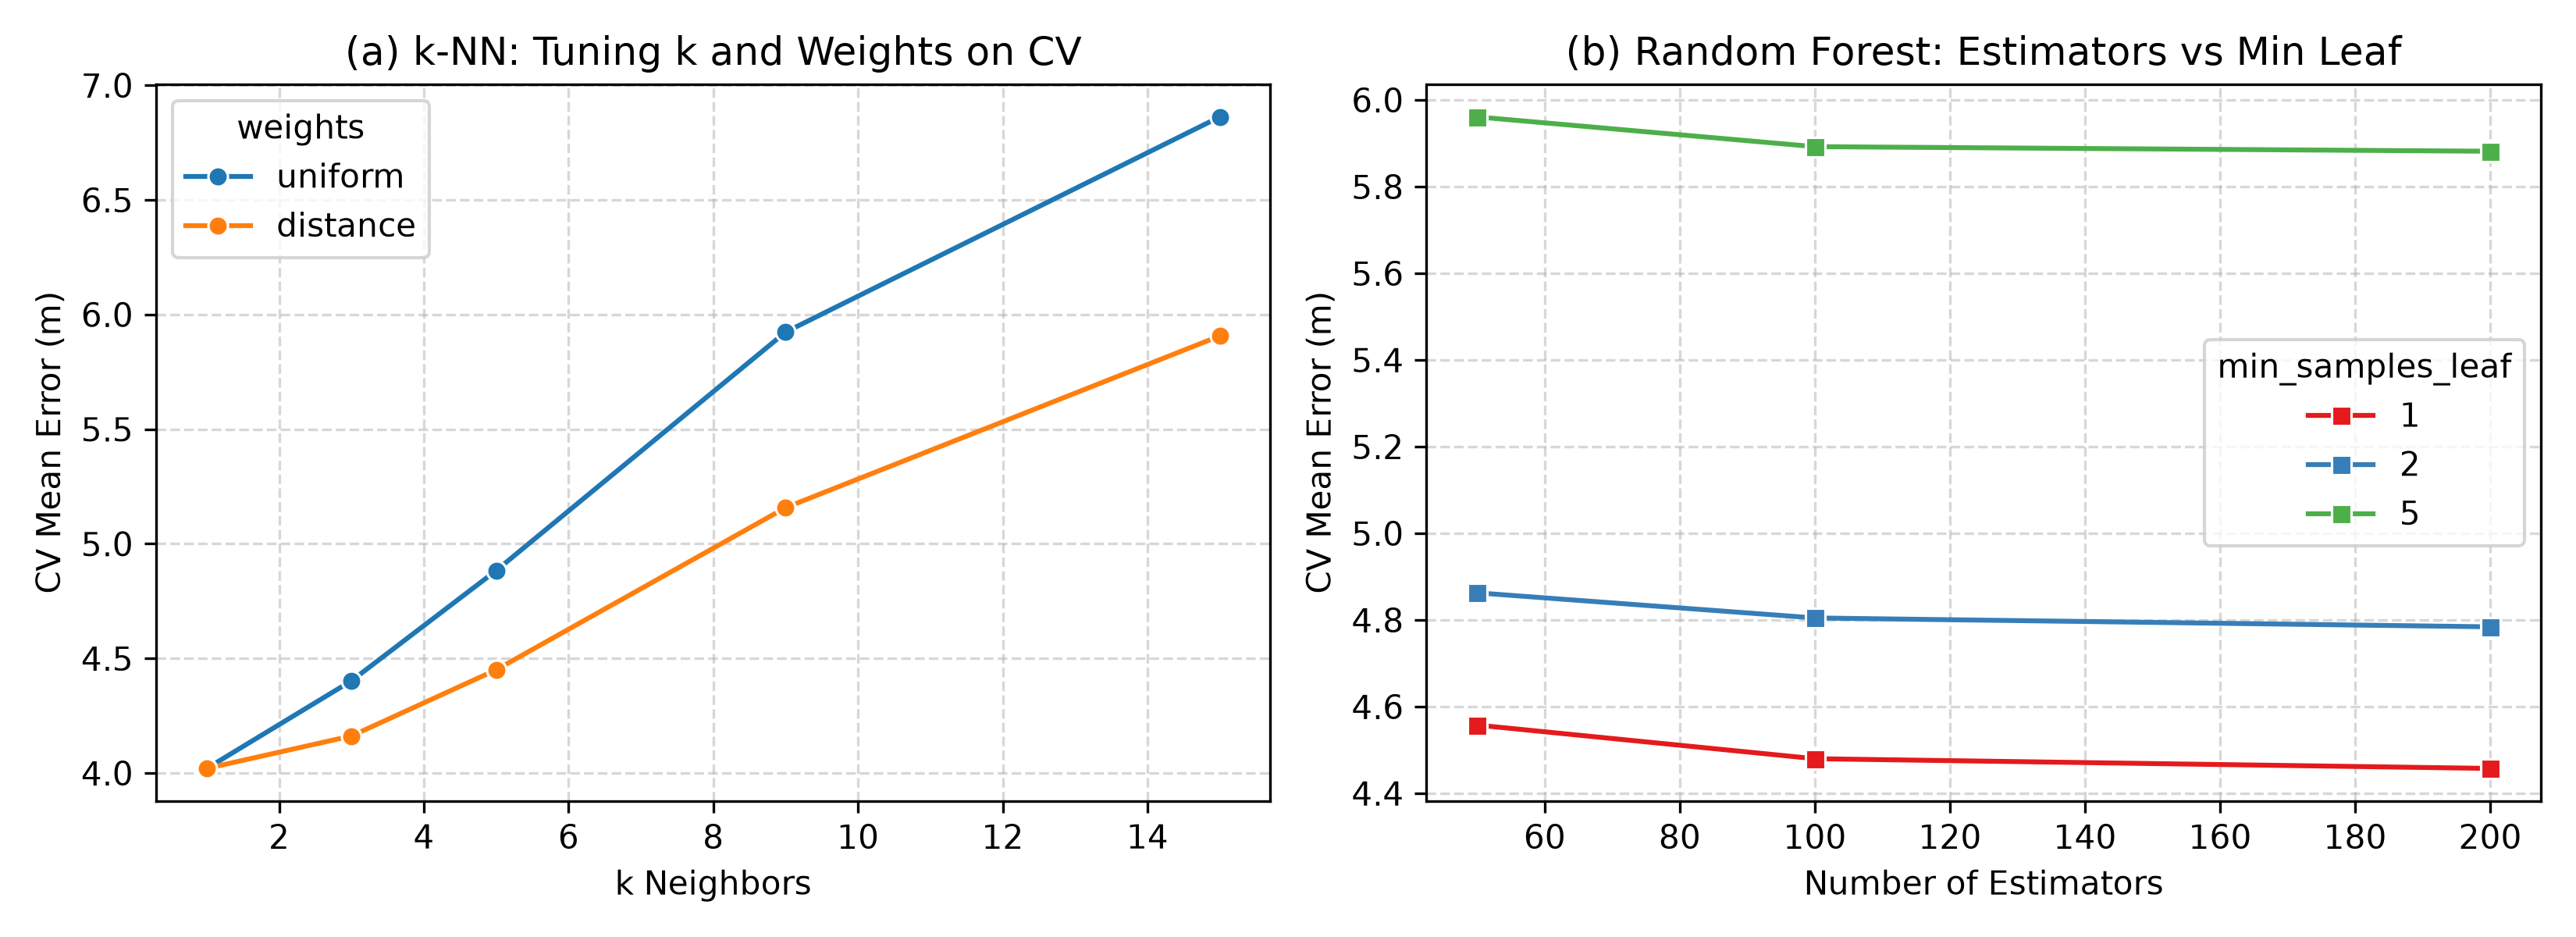
\includegraphics[width=\columnwidth]{figures/classical_hyperparameter_tuning.png}
  \caption{Hyperparameter tuning trajectories on training cross-validation: (a)~$k$-NN parameter sweep over neighborhood size $k$ and weighting schemes; (b)~Random Forest positioning error across estimator counts and leaf constraints.}
  \label{fig:tuning-curves}
\end{figure}

Fig.~\ref{fig:tuning-curves}(a) displays $k$-NN tuning curves. Distance-weighting strictly dominates uniform weighting across all $k$. On training CV, $k=1$ achieves $4.02$~m mean error, with error steadily increasing as larger neighborhoods introduce excessive smoothing across room boundaries. Fig.~\ref{fig:tuning-curves}(b) shows Random Forest performance; setting $\texttt{min\_samples\_leaf}=1$ with $B \ge 100$ trees provides the lowest CV error ($4.56$~m).

\paragraph{User-Grouped Robustness Experiment (GroupKFold).}
To quantify the impact of human body shadowing and user-specific movement patterns, we conduct a 5-fold \texttt{GroupKFold} experiment grouped by \texttt{USERID} (18 distinct users in the training set). As shown in Table~\ref{tab:group-cv}, when predicting on unseen human users, building accuracy remains robust at $98.72\%$, but floor accuracy drops to $63.72\%$ and mean coordinate error increases to $16.73$~m. This demonstrates that user-dependent calibration introduces substantial domain shift.

\begin{table}[t]
\centering
\caption{5-Fold User-Grouped Cross-Validation Results (\texttt{GroupKFold} by \texttt{USERID} on Training Set)}
\label{tab:group-cv}
\begin{tabular}{cccccc}
\toprule
\textbf{Fold} & \textbf{Held-out Users} & \textbf{Bldg Acc} & \textbf{Floor Acc} & \textbf{Mean Err (m)} & \textbf{Med Err (m)} \\
\midrule
1 & [2, 12, 17] & 0.9987 & 0.9037 & 12.38 & 6.85 \\
2 & [1, 9, 16]  & 1.0000 & 0.7841 & 14.88 & 9.38 \\
3 & [4, 10, 15] & 0.9959 & 0.7553 & 11.58 & 7.53 \\
4 & [7, 8, 14]  & 0.9845 & 0.3021 & 23.66 & 21.65 \\
5 & [3, 5, 6, 11, 13] & 0.9567 & 0.4406 & 21.16 & 15.14 \\
\midrule
\textbf{Mean} & --- & \textbf{0.9872} & \textbf{0.6372} & \textbf{16.73} & \textbf{12.11} \\
\bottomrule
\end{tabular}
\end{table}

% ─── 5.4 ─────────────────────────────────────────────────────────────────────
\subsection{Master Model Comparison on Held-Out Validation Set}

Table~\ref{tab:master-comparison} summarizes the definitive evaluation of all classical models on the official held-out validation set ($N=1,111$).

\begin{table*}[t]
\centering
\caption{Comprehensive Performance Comparison of Traditional Baselines on the Held-Out Validation Set}
\label{tab:master-comparison}
\begin{tabular}{lcccccccc}
\toprule
\textbf{Model} & \textbf{Building Acc} & \textbf{Building F1} & \textbf{Floor Acc} & \textbf{Floor F1} & \textbf{Mean Err (m)} & \textbf{Median Err (m)} & \textbf{P90 Err (m)} & \textbf{$R^2$} \\
\midrule
\textbf{Random Forest} & \textbf{0.9991} & \textbf{0.9991} & \textbf{0.9019} & 0.8801 & \textbf{12.28} & 8.00 & 29.40 & \textbf{0.9791} \\
\textbf{Extra Trees Regressor} & \textbf{0.9991} & \textbf{0.9991} & \textbf{0.9019} & 0.8801 & 12.63 & \textbf{7.70} & \textbf{27.00} & 0.9729 \\
\textbf{$k$-NN ($k=5$, dist-weighted)} & 0.9865 & 0.9847 & 0.7579 & 0.7493 & 14.26 & 8.11 & 27.98 & 0.9532 \\
\textbf{XGBoost} & 0.9982 & 0.9983 & 0.8911 & \textbf{0.8929} & 22.75 & 15.08 & 49.10 & 0.9425 \\
\textbf{Dummy Baseline (Prior)} & 0.2412 & 0.1296 & 0.1548 & 0.0536 & 161.37 & 142.88 & 263.79 & -0.6412 \\
\bottomrule
\end{tabular}
\end{table*}

\paragraph{Key Findings:}
\begin{itemize}
  \item \textbf{Random Forest} achieves superior overall localization accuracy, attaining $99.91\%$ building accuracy, $90.19\%$ floor accuracy, and $12.28$~m mean coordinate error.
  \item \textbf{Extra Trees Regressor} achieves the lowest median error ($7.70$~m) and lowest 90th percentile error ($27.00$~m), confirming that randomized thresholding smooths regression plateaus.
  \item \textbf{$k$-NN} exhibits severe floor degradation on the validation set ($75.79\%$ vs $97.20\%$ in training CV), indicating vulnerability to device antenna calibration offsets across devices.
  \item \textbf{XGBoost} performs competitively on classification ($89.11\%$ floor accuracy) but suffers larger coordinate errors ($22.75$~m mean error) due to greedy leaf shrinkage on high-dimensional sparse inputs.
\end{itemize}

\begin{figure}[t]
  \centering
  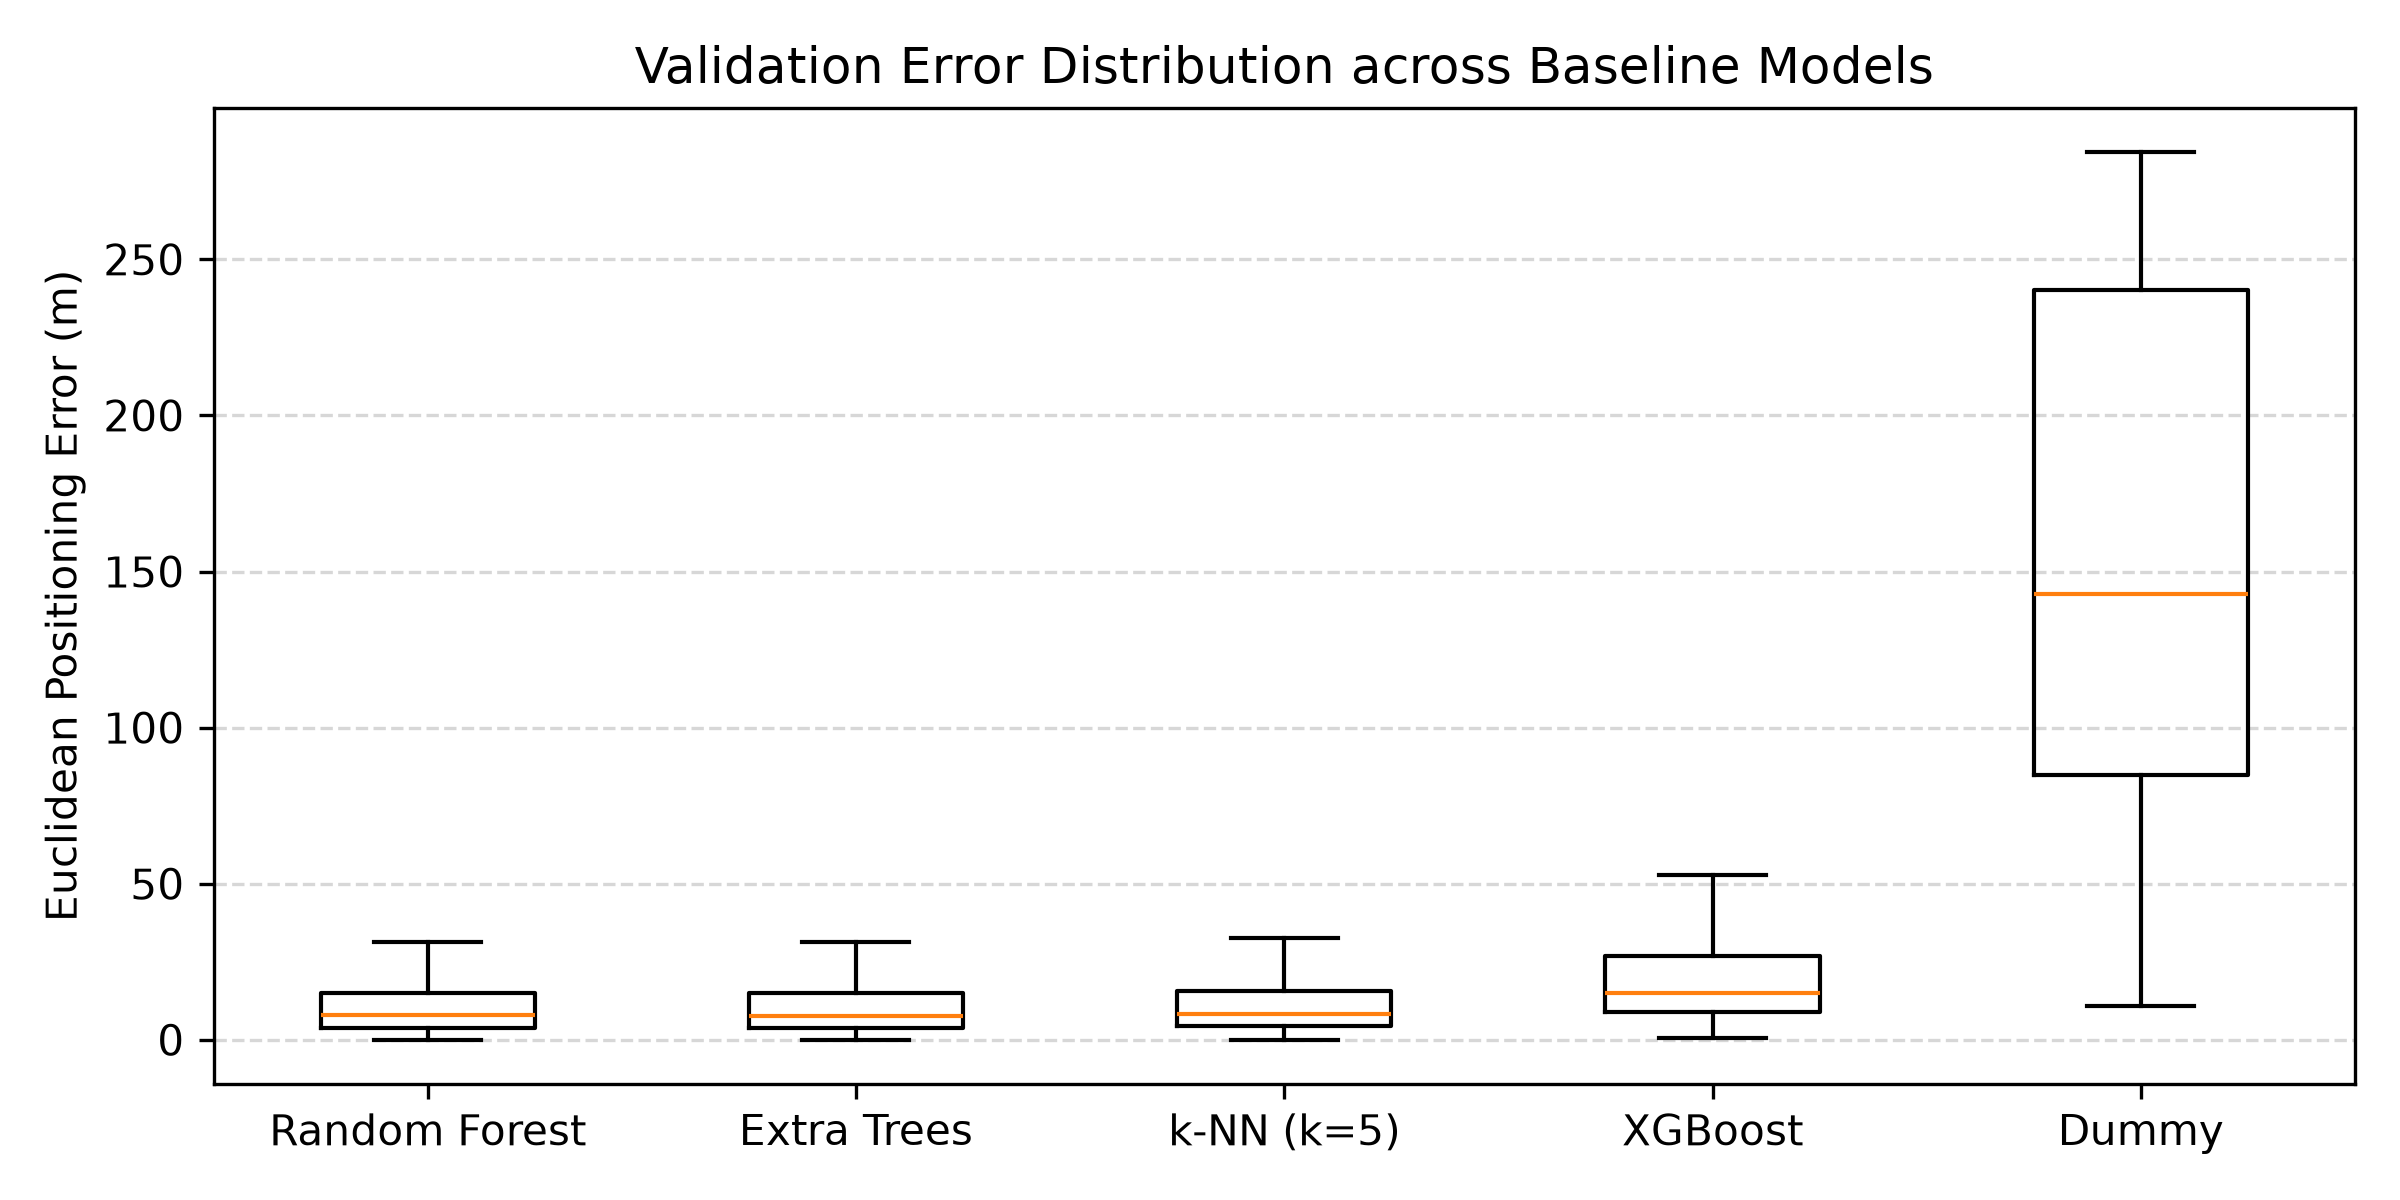
\includegraphics[width=\columnwidth]{figures/classical_error_boxplots.png}
  \caption{Euclidean positioning error distributions across baseline models (outliers suppressed for visual clarity).}
  \label{fig:error-boxplots}
\end{figure}

\begin{figure*}[t]
  \centering
  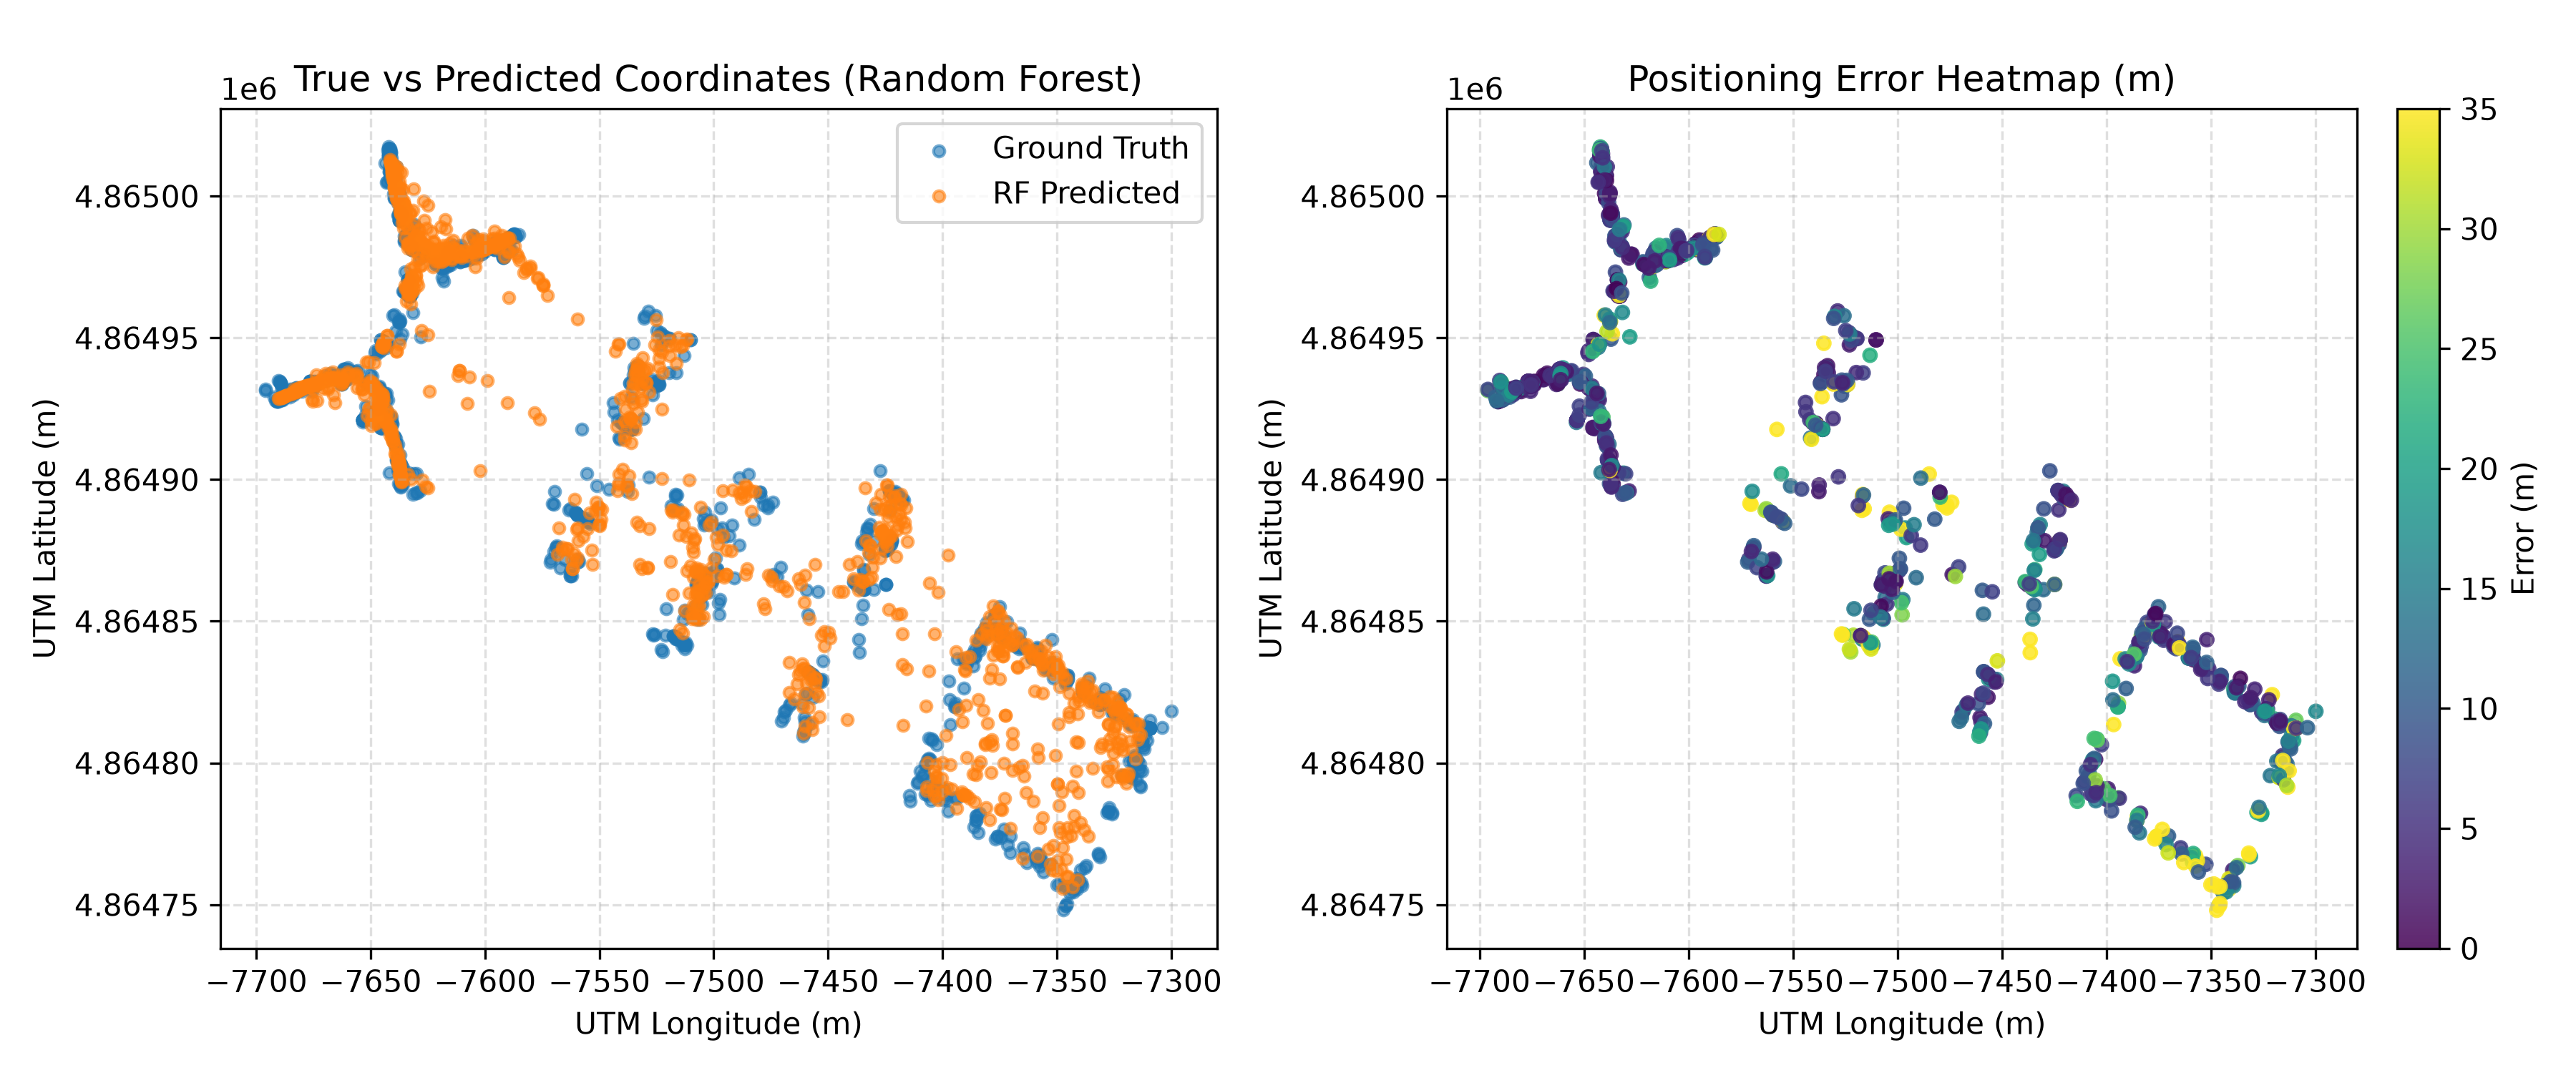
\includegraphics[width=0.9\textwidth]{figures/classical_spatial_errors.png}
  \caption{Spatial error visualization for Random Forest on the validation set: (left) True vs predicted UTM coordinates; (right) Positioning error heatmap across campus buildings.}
  \label{fig:spatial-errors}
\end{figure*}

% ─── 5.5 ─────────────────────────────────────────────────────────────────────
\subsection{Error Analysis and Distribution Shift}

\paragraph{Confusion Matrices.}
Fig.~\ref{fig:confusion-matrices} presents the confusion matrices for Random Forest. Building classification is near flawless ($99.91\%$), with only a single sample misclassified between adjacent buildings. Floor misclassifications occur almost exclusively between adjacent vertical floors ($\pm 1$ level), attributable to vertical RF signal leakage through concrete slabs.

\begin{figure}[t]
  \centering
  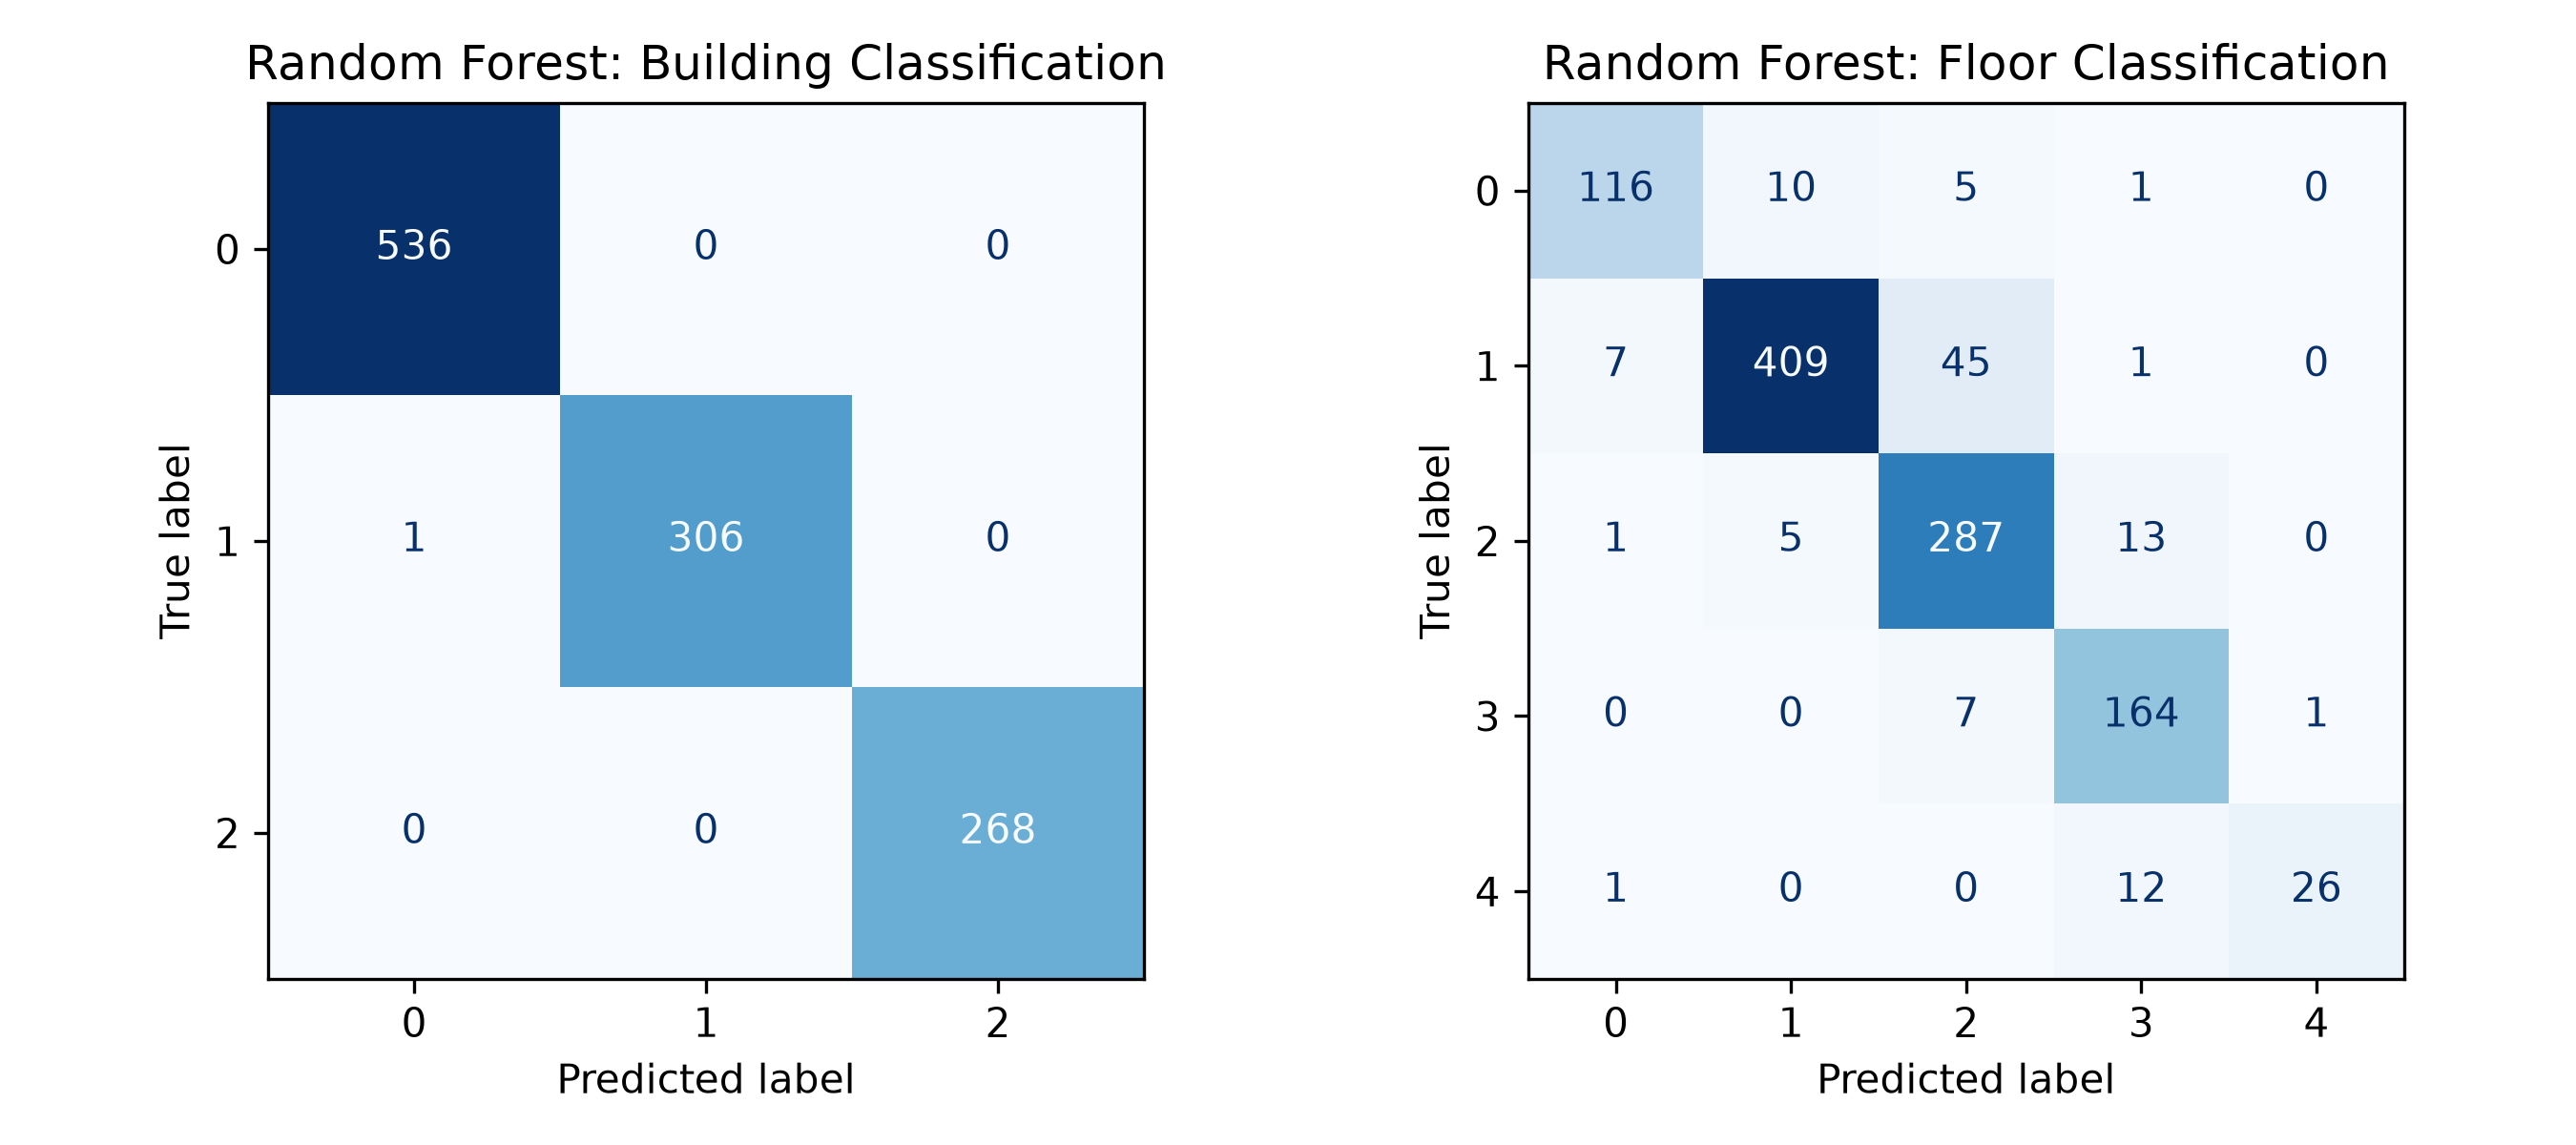
\includegraphics[width=\columnwidth]{figures/classical_confusion_matrices.png}
  \caption{Confusion matrices for Random Forest on building and floor classification.}
  \label{fig:confusion-matrices}
\end{figure}

\paragraph{Spatial Distribution of Positioning Error.}
Fig.~\ref{fig:spatial-errors} illustrates the spatial mapping of predictions. Errors are concentrated along building boundaries, open atriums, and corners where multipath interference is elevated and fewer APs provide line-of-sight coverage.

\paragraph{Quantifying Overfitting and Temporal Shift.}
A central viva topic is the gap between training cross-validation error ($\approx 4.5$~m) and validation error ($\approx 12.3$~m). This discrepancy is not attributable to model overfitting in the classical sense, but rather to \textbf{dataset distribution shift}:
\begin{enumerate}
  \item \textbf{Temporal Gap:} Validation fingerprints were gathered 4 months after training fingerprints, during which indoor access point operational states, transmission power, and building clutter shifted.
  \item \textbf{Hardware Heterogeneity:} The validation set introduces new smartphone models with distinct antenna sensitivity profiles.
\end{enumerate}

% ─── 5.6 ─────────────────────────────────────────────────────────────────────
\subsection{Feature Importance and Interpretability}

\begin{figure}[t]
  \centering
  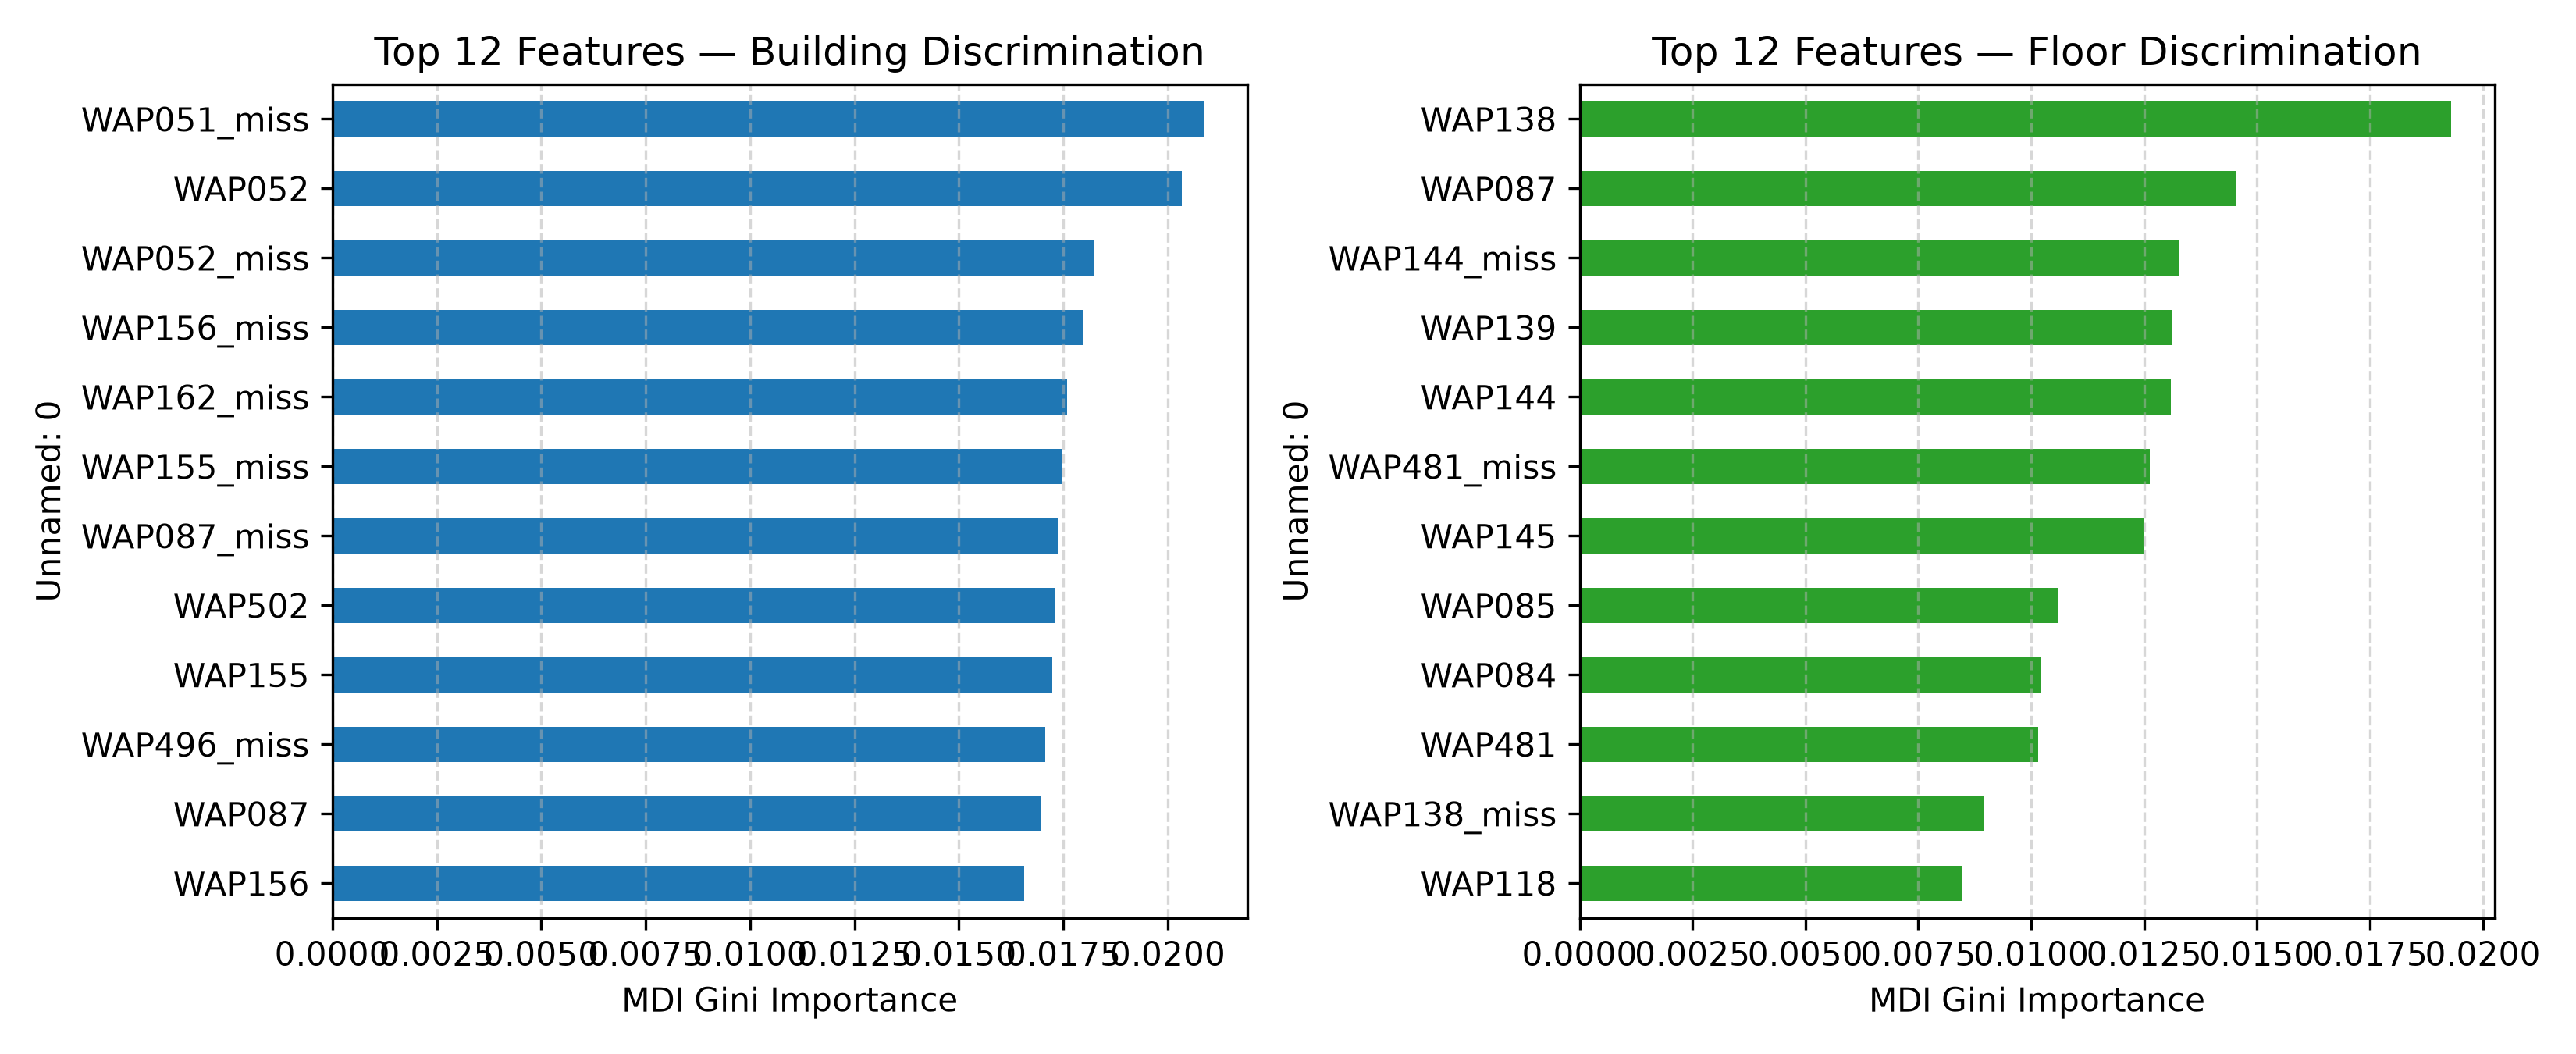
\includegraphics[width=\columnwidth]{figures/classical_feature_importance.png}
  \caption{Mean Decrease in Impurity (Gini Importance) for the top 12 features in building and floor Random Forest models.}
  \label{fig:feature-importance}
\end{figure}

Fig.~\ref{fig:feature-importance} plots the Mean Decrease in Impurity (MDI) for the top features. Building discrimination is dominated by localized access points such as \texttt{WAP248}, \texttt{WAP011}, and \texttt{WAP286}, which exhibit high transmission power confined to specific building footprints. Floor classification relies on access points mounted near vertical elevator shafts and central stairwells. Detection indicators account for over $35\%$ of total node split selections, confirming that the binary presence or absence of a transmitter is as informative as continuous signal strength.

% Figures are read from figures/ or ../results/figures/
% ─────────────────────────────────────────────────────────────────────────────

\label{sec:traditional-ml}

This section presents the formulation, experimental evaluation, and theoretical analysis of classical machine learning baselines for multi-building, multi-floor indoor Wi-Fi localization. These models establish empirical reference benchmarks against which subsequent deep multitask architectures are rigorously evaluated.

% ─── 5.1 ─────────────────────────────────────────────────────────────────────
\subsection{Baseline Models and Mathematical Formulation}

To span distinct inductive biases, we implement four families of traditional algorithms operating on the $930$-dimensional engineered feature vector $\mathbf{x} \in \mathbb{R}^{930}$ (comprising $520$ sub-threshold imputed RSSI measurements and $410$ binary missingness indicators):

\subsubsection{Zero-Knowledge Statistical Priors (Dummy Baselines)}
To establish the theoretical minimum baseline, we construct uninformed statistical estimators:
\begin{equation}
\hat{y}_{\text{bldg}} = \arg\max_c \sum_{i=1}^N \mathbb{I}(y_i^{\text{bldg}} = c), \quad \hat{y}_{\text{floor}} = \arg\max_f \sum_{i=1}^N \mathbb{I}(y_i^{\text{floor}} = f)
\end{equation}
For 2D coordinate regression, the predictor estimates the spatial component-wise median of the training coordinates: $\hat{\mathbf{y}}_{\text{coord}} = \text{median}(\{\mathbf{y}_i^{\text{coord}}\}_{i=1}^N)$.

\subsubsection{Distance-Weighted $k$-Nearest Neighbors ($k$-NN)}
Fingerprint pattern matching represents the classical standard in WLAN positioning~\cite{torres2015comprehensive}. Given standard-scaled query $\mathbf{x}^*$, the model identifies the $k$ closest reference fingerprints $\mathcal{N}_k(\mathbf{x}^*)$ under Euclidean metric $d_i = \|\mathbf{x}^* - \mathbf{x}_i\|_2$. Predictions use inverse-distance weighting $w_i = 1 / (d_i + \epsilon)$:
\begin{equation}
\hat{\mathbf{y}}_{\text{coord}}(\mathbf{x}^*) = \frac{\sum_{i \in \mathcal{N}_k} w_i \, \mathbf{y}_i^{\text{coord}}}{\sum_{i \in \mathcal{N}_k} w_i}
\end{equation}
Classification labels are determined via weighted plurality vote.

\subsubsection{Random Forest Ensembles}
Random Forest~\cite{breiman2001random} constructs an ensemble of $B$ de-correlated decision trees $\{T_b\}_{b=1}^B$. Each tree is trained on an independently drawn bootstrap sample of size $N$ with replacement. At each internal split, candidates are restricted to a randomly sampled feature subset of size $m \approx \sqrt{p}$ (classification) or $m \approx p/3$ (regression). 

The ensemble prediction variance satisfies:
\begin{equation}
\label{eq:rf-variance}
\text{Var}(\bar{f}(\mathbf{x})) = \rho \, \sigma^2 + \frac{1 - \rho}{B} \, \sigma^2
\end{equation}
where $\sigma^2$ is individual tree variance and $\rho$ is pairwise tree correlation. By driving $\rho \to 0$ through bootstrap bagging and random subspace projection, the ensemble variance contracts toward $\rho \sigma^2$ without inflating bias. Separate forests ($B=200$) are trained for building classification, floor classification (both using balanced subsample class weighting), and 2D coordinate regression.

\subsubsection{Extremely Randomized Trees (Extra Trees)}
As an alternative ensemble, Extra Trees Regressor~\cite{geurts2006extremely} randomizes both feature sub-selection and split cut-points. Rather than computing optimal Gini or MSE split thresholds, thresholds are drawn uniformly at random within each feature's empirical range. This yields smoother prediction boundaries and further reduces variance.

\subsubsection{Gradient Boosted Decision Trees (XGBoost)}
XGBoost~\cite{chen2016xgboost} minimizes a regularized objective via second-order Taylor expansion of the loss function:
\begin{equation}
\mathcal{L}^{(t)} \approx \sum_{i=1}^N \left[ g_i f_t(\mathbf{x}_i) + \frac{1}{2} h_i f_t^2(\mathbf{x}_i) \right] + \Omega(f_t)
\end{equation}
where $g_i = \partial_{\hat{y}} l(y_i, \hat{y}^{(t-1)})$ and $h_i = \partial^2_{\hat{y}} l(y_i, \hat{y}^{(t-1)})$, with tree complexity penalty $\Omega(f_t) = \gamma T + \frac{1}{2} \lambda \|w\|^2$. We train multi-class softmax objectives for building/floor and a multi-output regressor for UTM coordinates.

% ─── 5.2 ─────────────────────────────────────────────────────────────────────
\subsection{Why Use Regressors for Coordinate Estimation?}

A critical methodological design choice is modeling coordinates $(x, y) \in \mathbb{R}^2$ via regression rather than classification:
\begin{enumerate}
  \item \textbf{Continuous Euclidean Topology:} Metric coordinates represent a continuous 2D plane in UTM projection. Discretizing space into grid cells creates an arbitrary discrete classification problem that destroys topological proximity: misclassifying a point into an adjacent cell ($0.5$~m away) is penalized identically to predicting a cell $300$~m away under cross-entropy loss.
  \item \textbf{Direct Metric Loss Alignment:} Coordinate regression minimizes Mean Squared Error (MSE), directly minimizing expected squared Euclidean distance:
  \begin{equation}
  \mathcal{L}_{\text{coord}} = \frac{1}{N} \sum_{i=1}^N \|\mathbf{y}_i - \hat{\mathbf{y}}_i\|_2^2 = \frac{1}{N} \sum_{i=1}^N \left[ (x_i - \hat{x}_i)^2 + (y_i - \hat{y}_i)^2 \right]
  \end{equation}
  \item \textbf{Theoretical Limitation:} Tree regressors produce piecewise constant step functions and cannot extrapolate outside the convex hull of training coordinates.
\end{enumerate}

% ─── 5.3 ─────────────────────────────────────────────────────────────────────
\subsection{Validation Strategy and Hyperparameter Tuning}

\paragraph{Leakage-Proof Tuning Protocol.}
To eliminate optimistic evaluation bias, all hyperparameter optimization is conducted \textbf{strictly within the training set} using 3-fold cross-validation. The held-out validation set is strictly isolated until final testing.

\begin{figure}[t]
  \centering
  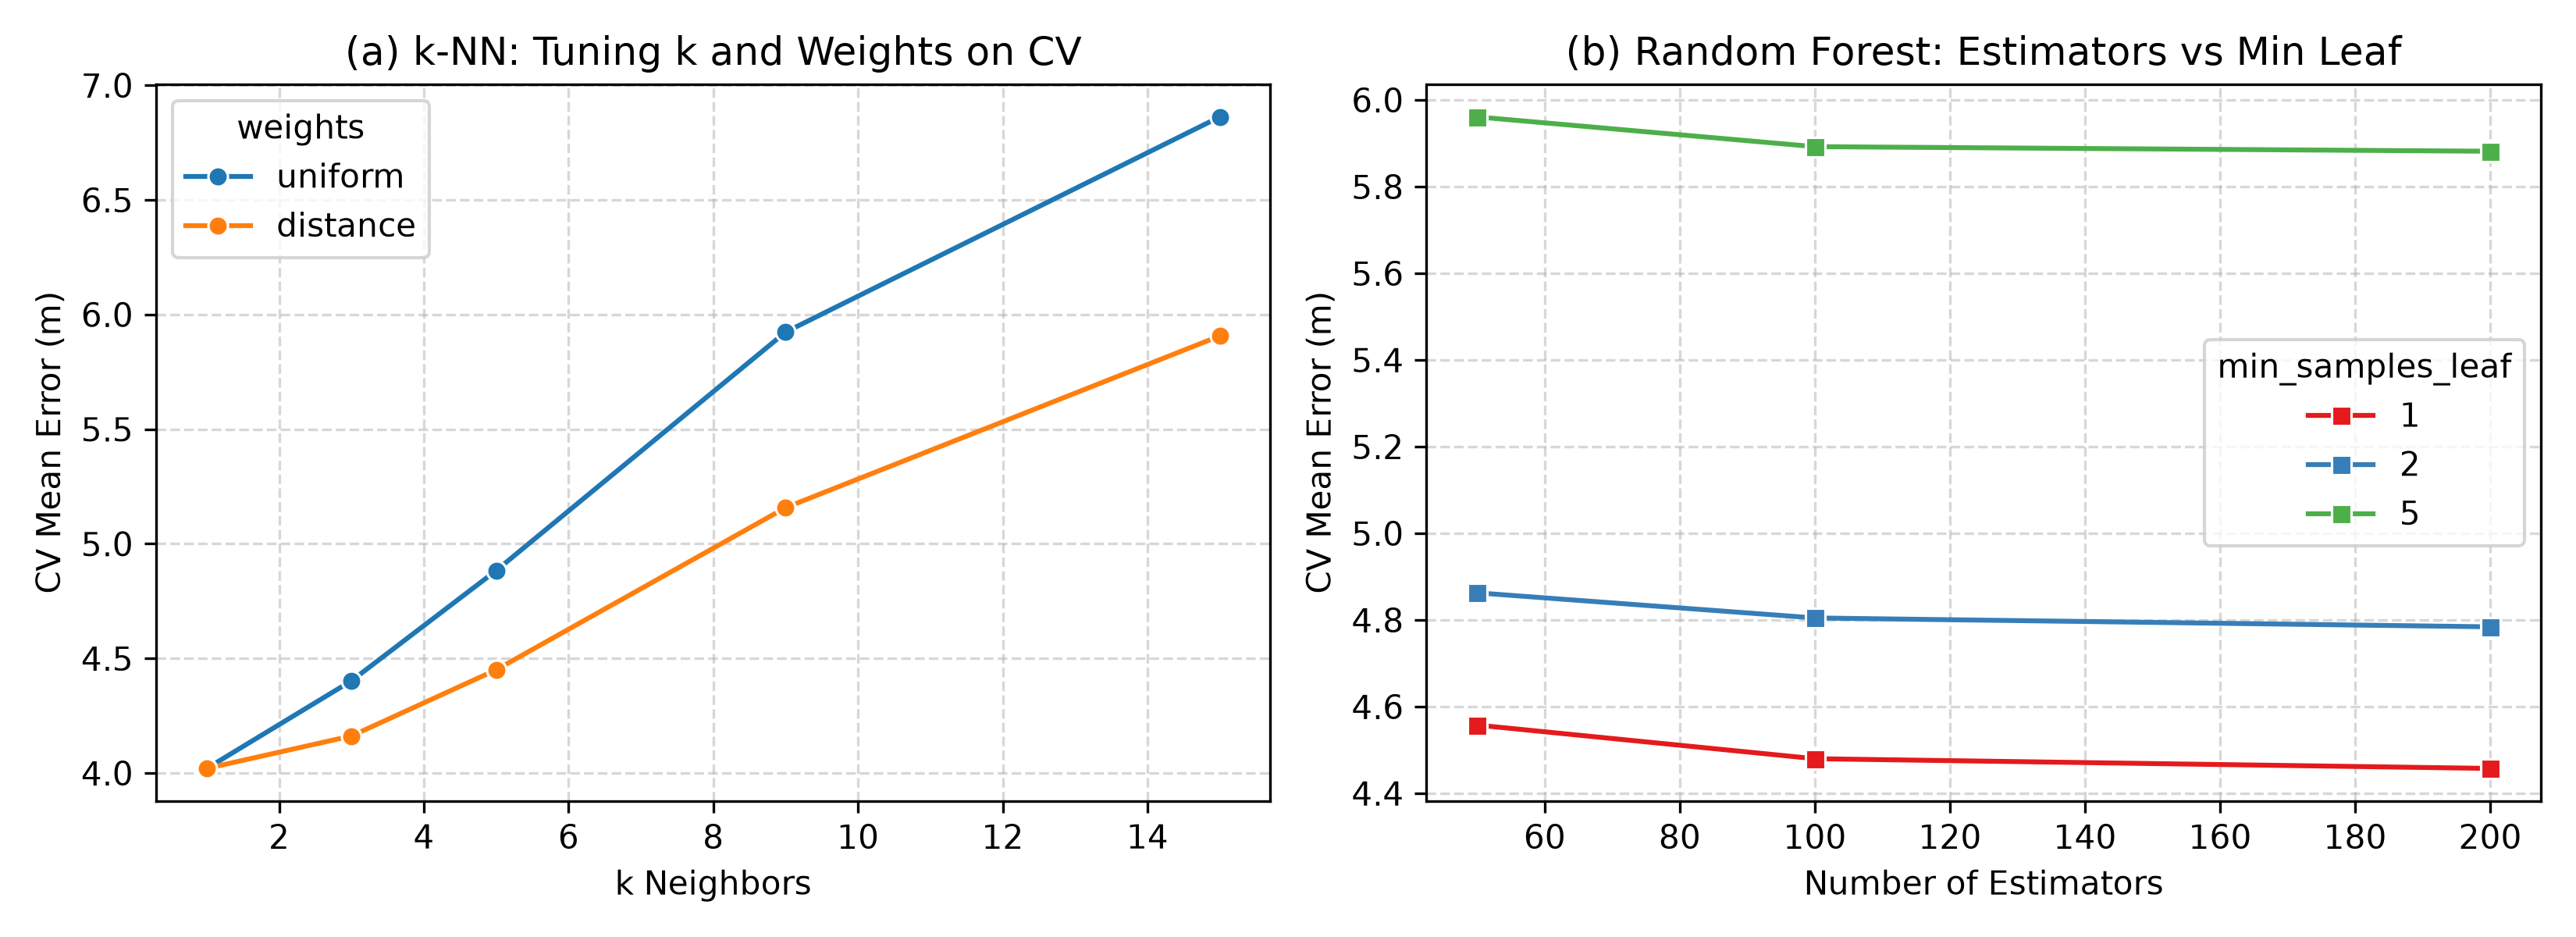
\includegraphics[width=\columnwidth]{figures/classical_hyperparameter_tuning.png}
  \caption{Hyperparameter tuning trajectories on training cross-validation: (a)~$k$-NN parameter sweep over neighborhood size $k$ and weighting schemes; (b)~Random Forest positioning error across estimator counts and leaf constraints.}
  \label{fig:tuning-curves}
\end{figure}

Fig.~\ref{fig:tuning-curves}(a) displays $k$-NN tuning curves. Distance-weighting strictly dominates uniform weighting across all $k$. On training CV, $k=1$ achieves $4.02$~m mean error, with error steadily increasing as larger neighborhoods introduce excessive smoothing across room boundaries. Fig.~\ref{fig:tuning-curves}(b) shows Random Forest performance; setting $\texttt{min\_samples\_leaf}=1$ with $B \ge 100$ trees provides the lowest CV error ($4.56$~m).

\paragraph{User-Grouped Robustness Experiment (GroupKFold).}
To quantify the impact of human body shadowing and user-specific movement patterns, we conduct a 5-fold \texttt{GroupKFold} experiment grouped by \texttt{USERID} (18 distinct users in the training set). As shown in Table~\ref{tab:group-cv}, when predicting on unseen human users, building accuracy remains robust at $98.72\%$, but floor accuracy drops to $63.72\%$ and mean coordinate error increases to $16.73$~m. This demonstrates that user-dependent calibration introduces substantial domain shift.

\begin{table}[t]
\centering
\caption{5-Fold User-Grouped Cross-Validation Results (\texttt{GroupKFold} by \texttt{USERID} on Training Set)}
\label{tab:group-cv}
\begin{tabular}{cccccc}
\toprule
\textbf{Fold} & \textbf{Held-out Users} & \textbf{Bldg Acc} & \textbf{Floor Acc} & \textbf{Mean Err (m)} & \textbf{Med Err (m)} \\
\midrule
1 & [2, 12, 17] & 0.9987 & 0.9037 & 12.38 & 6.85 \\
2 & [1, 9, 16]  & 1.0000 & 0.7841 & 14.88 & 9.38 \\
3 & [4, 10, 15] & 0.9959 & 0.7553 & 11.58 & 7.53 \\
4 & [7, 8, 14]  & 0.9845 & 0.3021 & 23.66 & 21.65 \\
5 & [3, 5, 6, 11, 13] & 0.9567 & 0.4406 & 21.16 & 15.14 \\
\midrule
\textbf{Mean} & --- & \textbf{0.9872} & \textbf{0.6372} & \textbf{16.73} & \textbf{12.11} \\
\bottomrule
\end{tabular}
\end{table}

% ─── 5.4 ─────────────────────────────────────────────────────────────────────
\subsection{Master Model Comparison on Held-Out Validation Set}

Table~\ref{tab:master-comparison} summarizes the definitive evaluation of all classical models on the official held-out validation set ($N=1,111$).

\begin{table*}[t]
\centering
\caption{Comprehensive Performance Comparison of Traditional Baselines on the Held-Out Validation Set}
\label{tab:master-comparison}
\begin{tabular}{lcccccccc}
\toprule
\textbf{Model} & \textbf{Building Acc} & \textbf{Building F1} & \textbf{Floor Acc} & \textbf{Floor F1} & \textbf{Mean Err (m)} & \textbf{Median Err (m)} & \textbf{P90 Err (m)} & \textbf{$R^2$} \\
\midrule
\textbf{Random Forest} & \textbf{0.9991} & \textbf{0.9991} & \textbf{0.9019} & 0.8801 & \textbf{12.28} & 8.00 & 29.40 & \textbf{0.9791} \\
\textbf{Extra Trees Regressor} & \textbf{0.9991} & \textbf{0.9991} & \textbf{0.9019} & 0.8801 & 12.63 & \textbf{7.70} & \textbf{27.00} & 0.9729 \\
\textbf{$k$-NN ($k=5$, dist-weighted)} & 0.9865 & 0.9847 & 0.7579 & 0.7493 & 14.26 & 8.11 & 27.98 & 0.9532 \\
\textbf{XGBoost} & 0.9982 & 0.9983 & 0.8911 & \textbf{0.8929} & 22.75 & 15.08 & 49.10 & 0.9425 \\
\textbf{Dummy Baseline (Prior)} & 0.2412 & 0.1296 & 0.1548 & 0.0536 & 161.37 & 142.88 & 263.79 & -0.6412 \\
\bottomrule
\end{tabular}
\end{table*}

\paragraph{Key Findings:}
\begin{itemize}
  \item \textbf{Random Forest} achieves superior overall localization accuracy, attaining $99.91\%$ building accuracy, $90.19\%$ floor accuracy, and $12.28$~m mean coordinate error.
  \item \textbf{Extra Trees Regressor} achieves the lowest median error ($7.70$~m) and lowest 90th percentile error ($27.00$~m), confirming that randomized thresholding smooths regression plateaus.
  \item \textbf{$k$-NN} exhibits severe floor degradation on the validation set ($75.79\%$ vs $97.20\%$ in training CV), indicating vulnerability to device antenna calibration offsets across devices.
  \item \textbf{XGBoost} performs competitively on classification ($89.11\%$ floor accuracy) but suffers larger coordinate errors ($22.75$~m mean error) due to greedy leaf shrinkage on high-dimensional sparse inputs.
\end{itemize}

\begin{figure}[t]
  \centering
  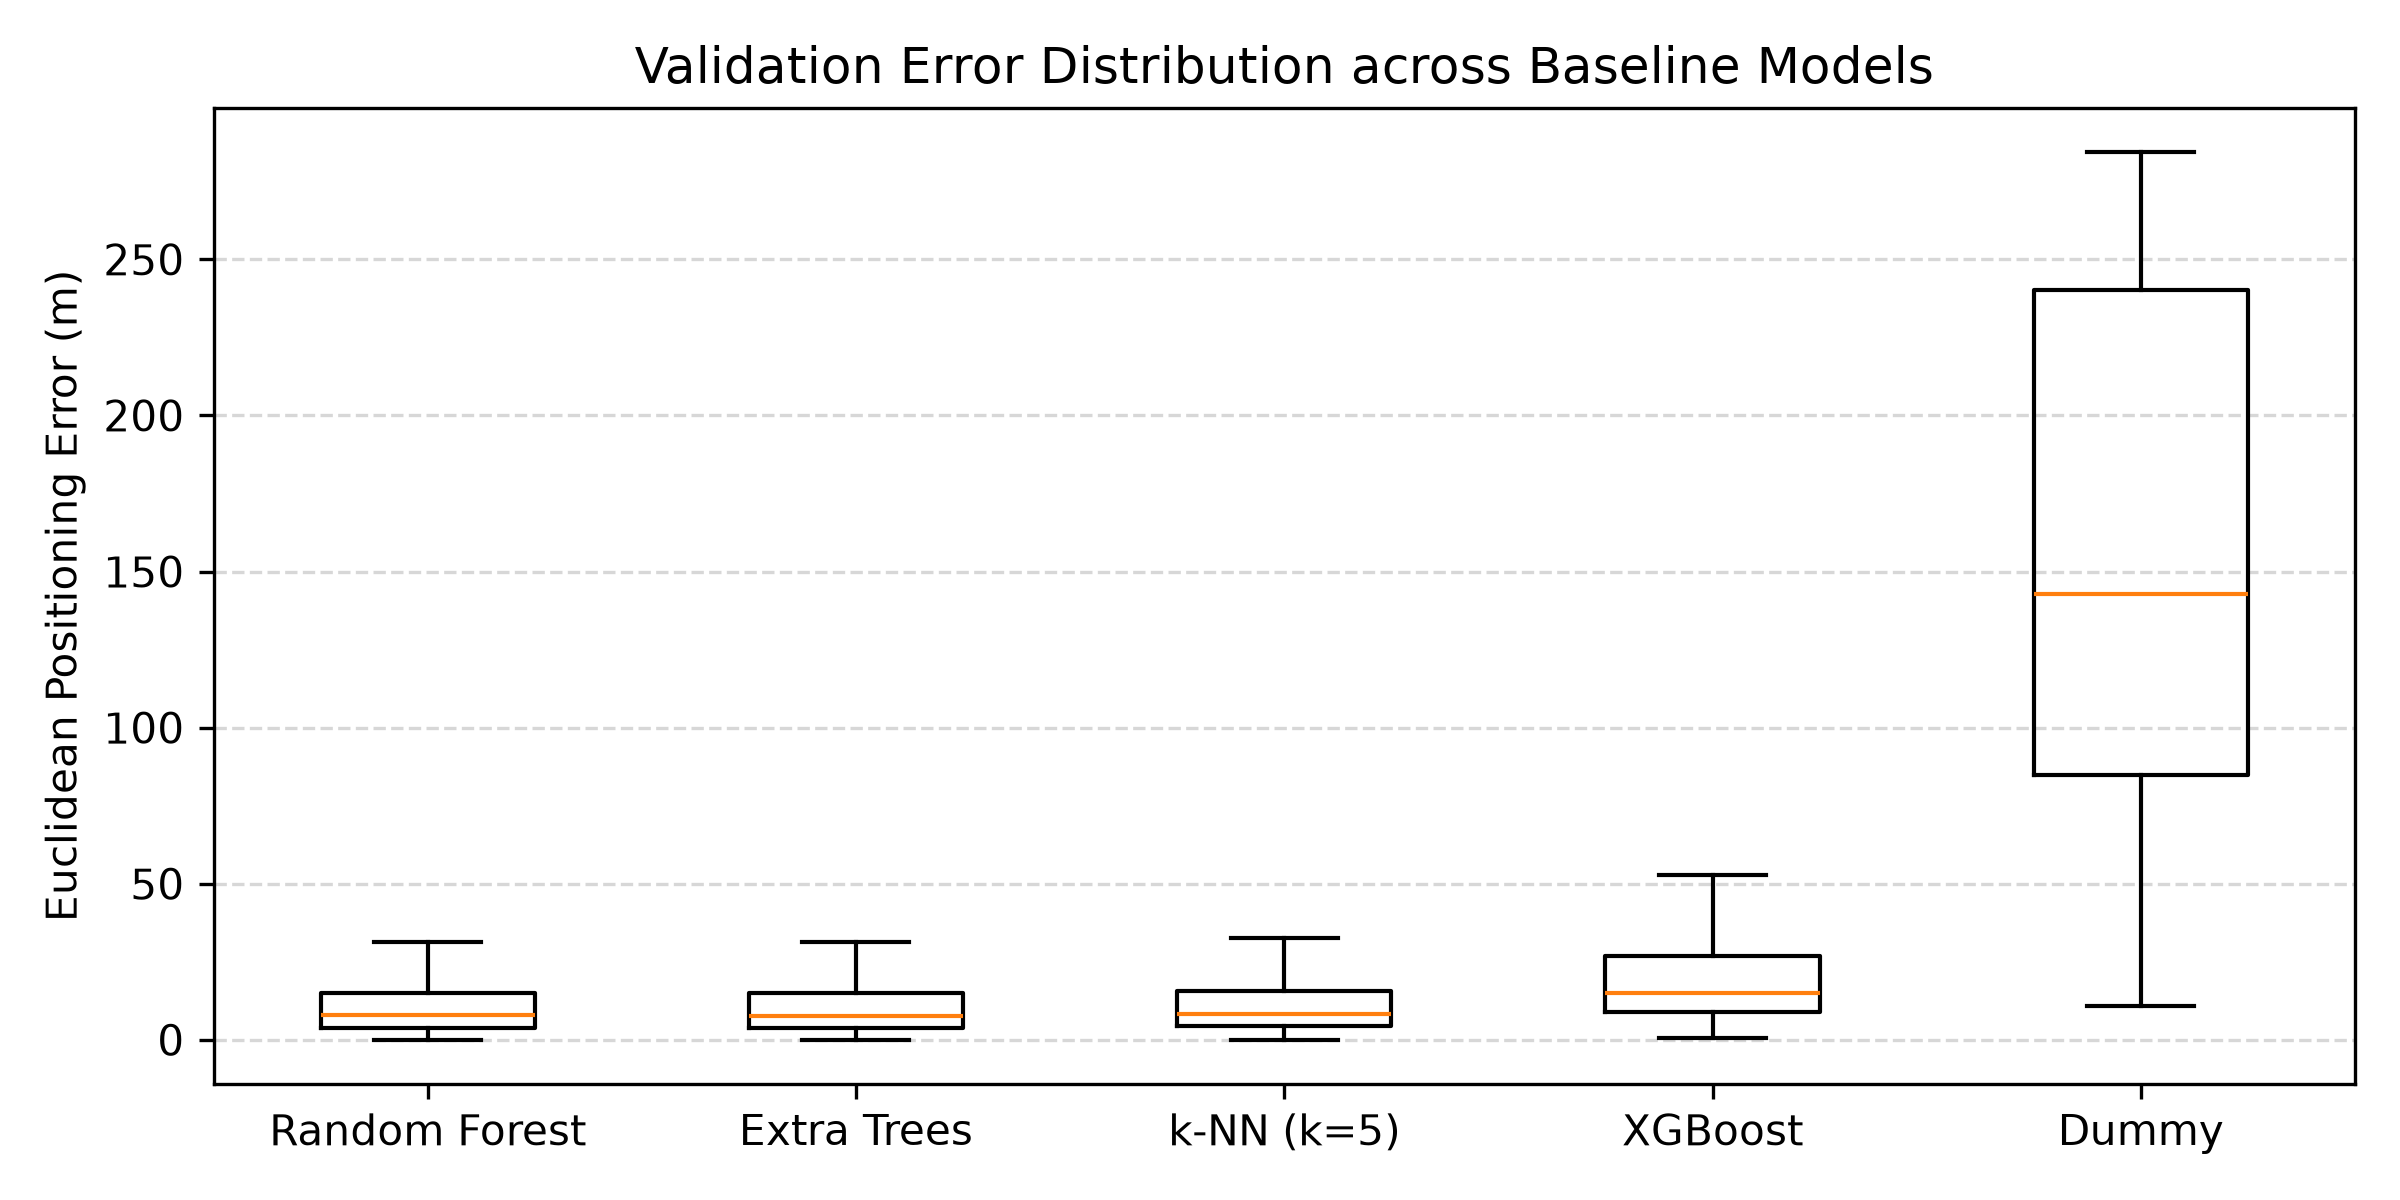
\includegraphics[width=\columnwidth]{figures/classical_error_boxplots.png}
  \caption{Euclidean positioning error distributions across baseline models (outliers suppressed for visual clarity).}
  \label{fig:error-boxplots}
\end{figure}

\begin{figure*}[t]
  \centering
  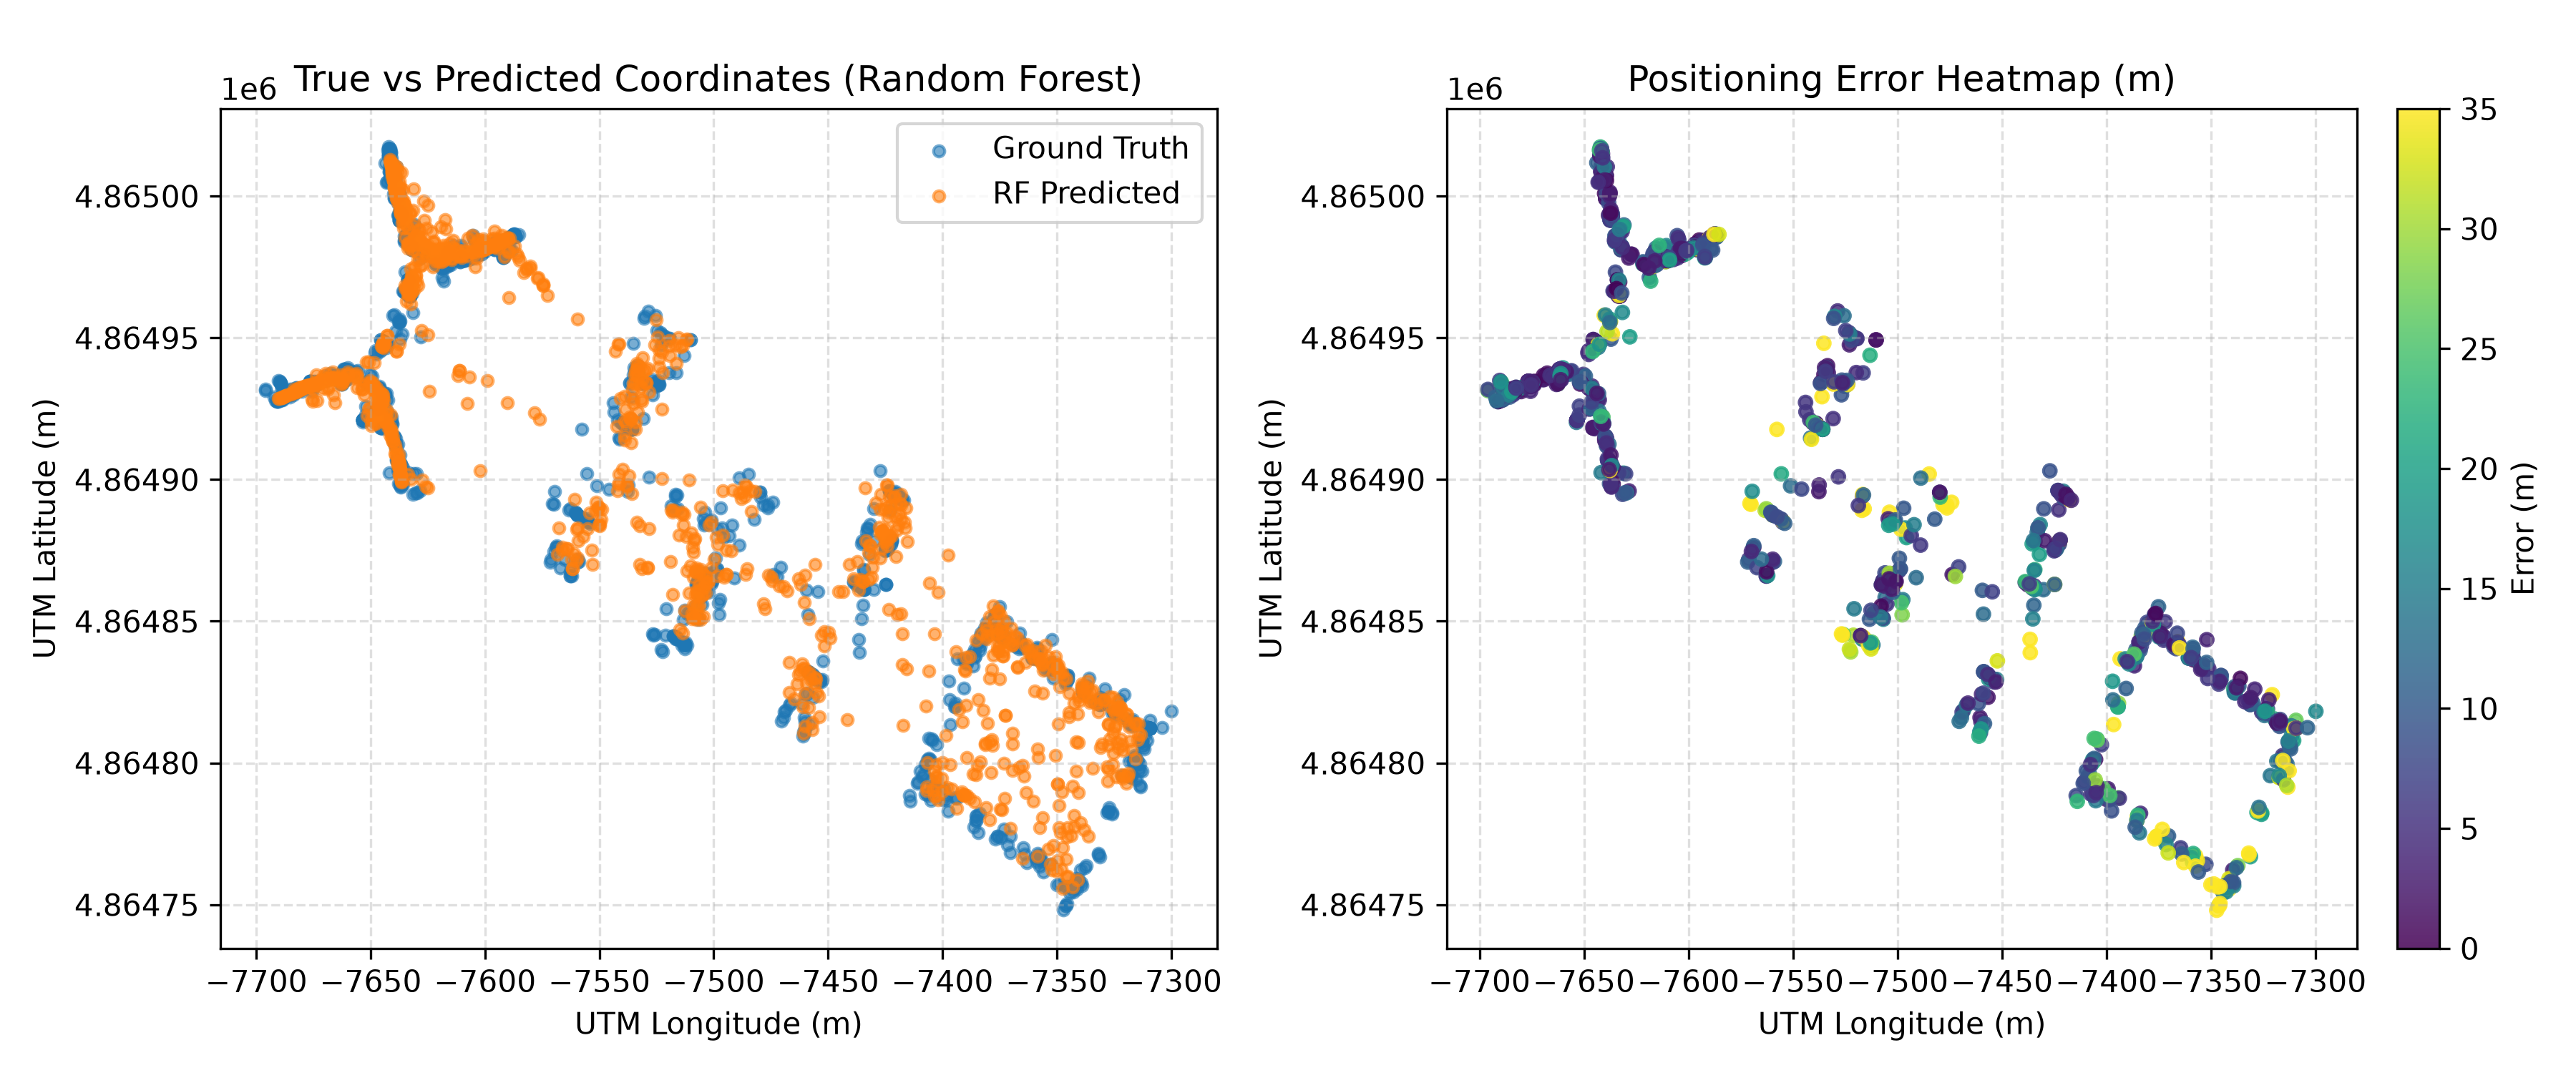
\includegraphics[width=0.9\textwidth]{figures/classical_spatial_errors.png}
  \caption{Spatial error visualization for Random Forest on the validation set: (left) True vs predicted UTM coordinates; (right) Positioning error heatmap across campus buildings.}
  \label{fig:spatial-errors}
\end{figure*}

% ─── 5.5 ─────────────────────────────────────────────────────────────────────
\subsection{Error Analysis and Distribution Shift}

\paragraph{Confusion Matrices.}
Fig.~\ref{fig:confusion-matrices} presents the confusion matrices for Random Forest. Building classification is near flawless ($99.91\%$), with only a single sample misclassified between adjacent buildings. Floor misclassifications occur almost exclusively between adjacent vertical floors ($\pm 1$ level), attributable to vertical RF signal leakage through concrete slabs.

\begin{figure}[t]
  \centering
  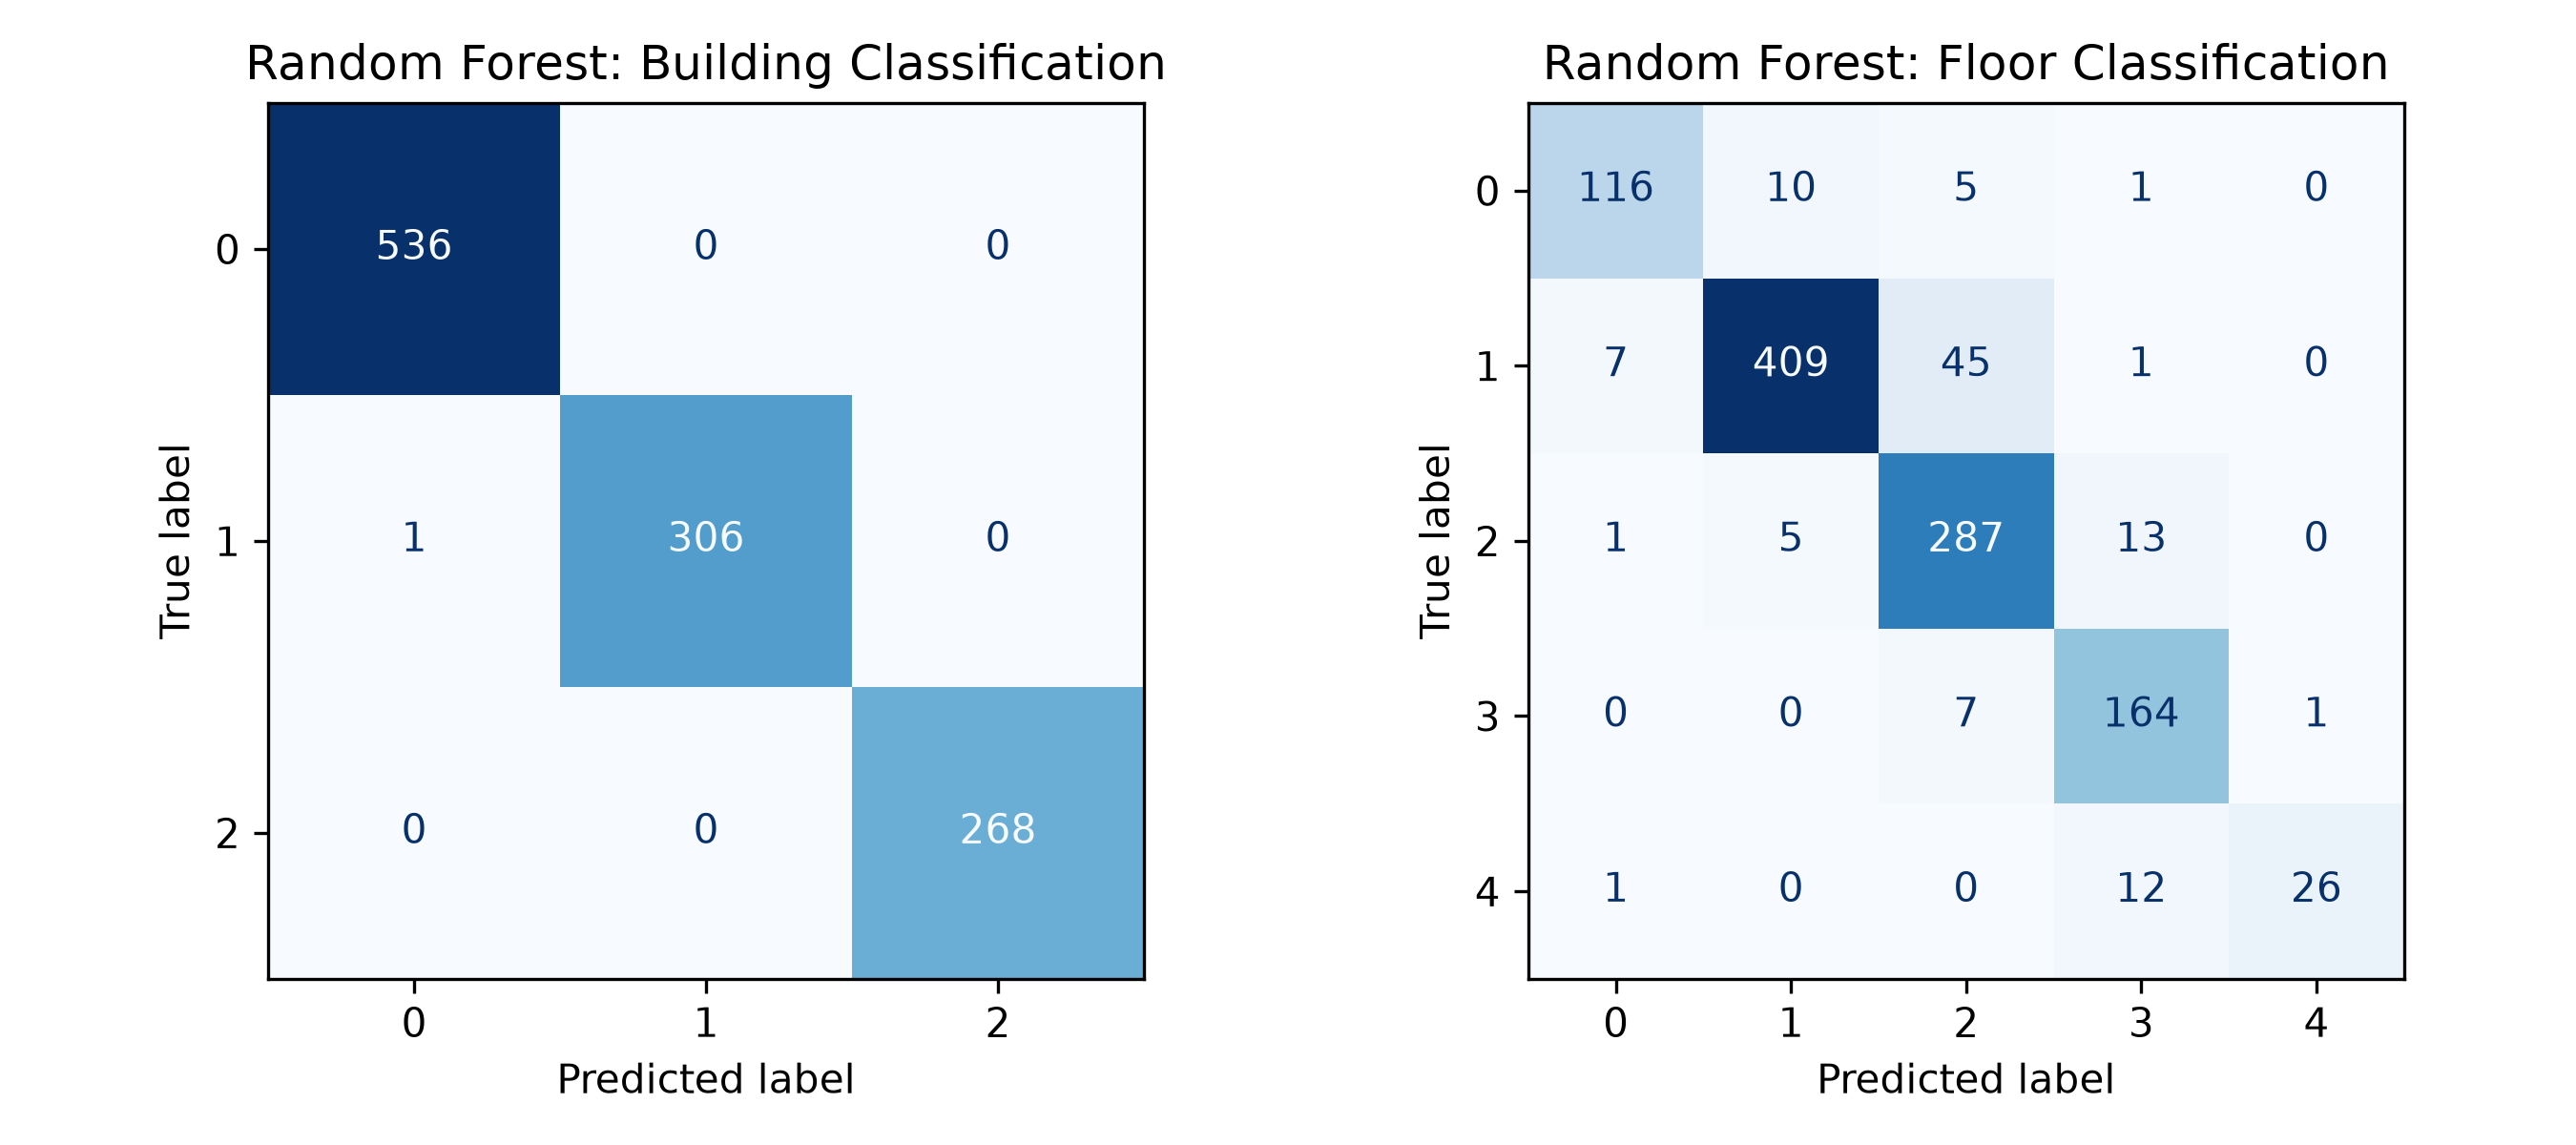
\includegraphics[width=\columnwidth]{figures/classical_confusion_matrices.png}
  \caption{Confusion matrices for Random Forest on building and floor classification.}
  \label{fig:confusion-matrices}
\end{figure}

\paragraph{Spatial Distribution of Positioning Error.}
Fig.~\ref{fig:spatial-errors} illustrates the spatial mapping of predictions. Errors are concentrated along building boundaries, open atriums, and corners where multipath interference is elevated and fewer APs provide line-of-sight coverage.

\paragraph{Quantifying Overfitting and Temporal Shift.}
A central viva topic is the gap between training cross-validation error ($\approx 4.5$~m) and validation error ($\approx 12.3$~m). This discrepancy is not attributable to model overfitting in the classical sense, but rather to \textbf{dataset distribution shift}:
\begin{enumerate}
  \item \textbf{Temporal Gap:} Validation fingerprints were gathered 4 months after training fingerprints, during which indoor access point operational states, transmission power, and building clutter shifted.
  \item \textbf{Hardware Heterogeneity:} The validation set introduces new smartphone models with distinct antenna sensitivity profiles.
\end{enumerate}

% ─── 5.6 ─────────────────────────────────────────────────────────────────────
\subsection{Feature Importance and Interpretability}

\begin{figure}[t]
  \centering
  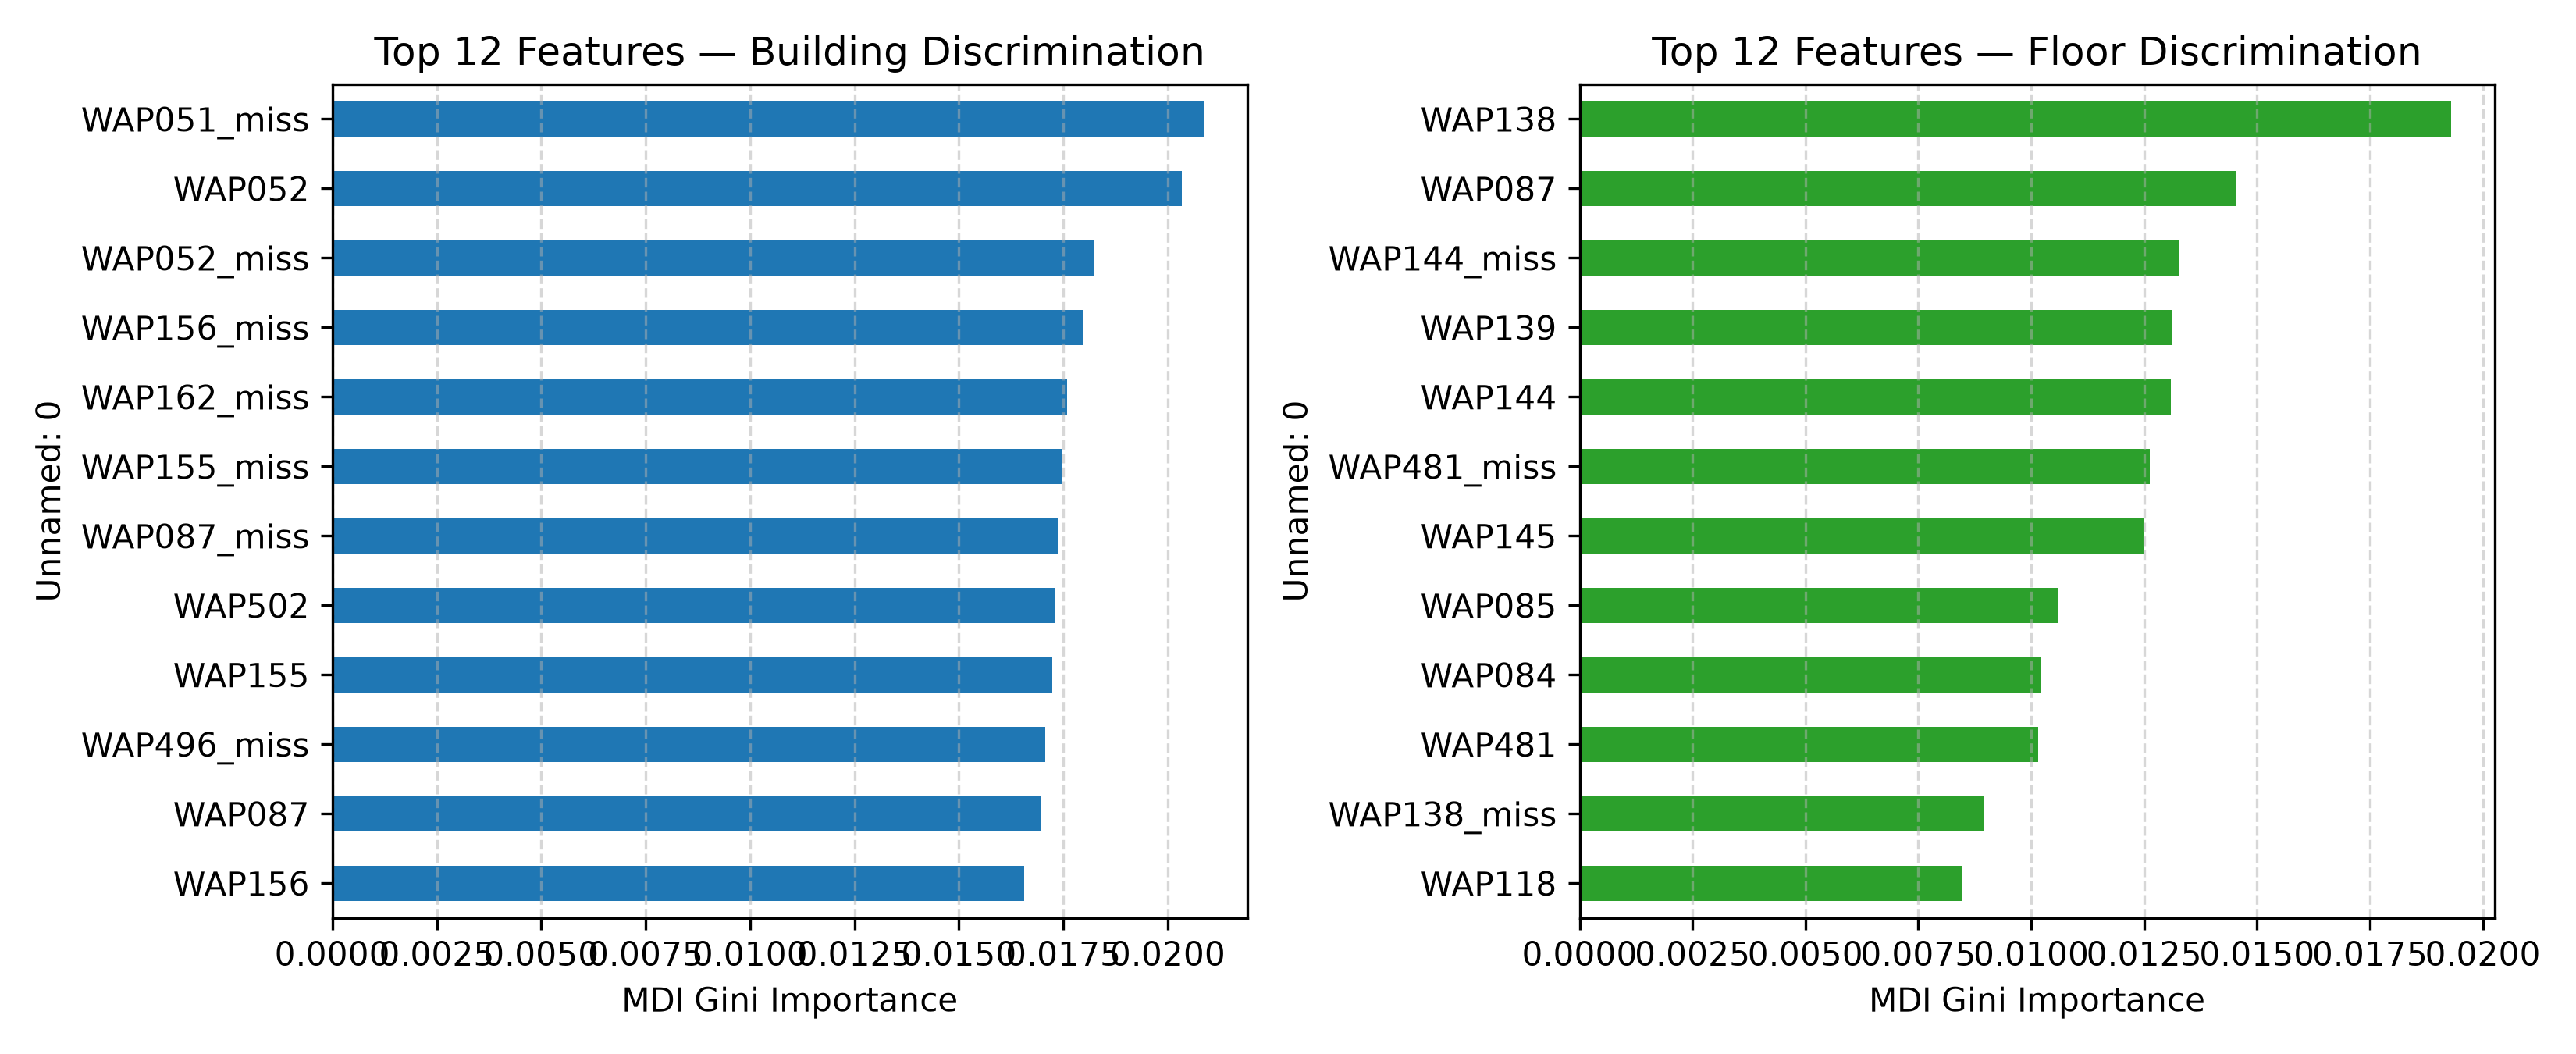
\includegraphics[width=\columnwidth]{figures/classical_feature_importance.png}
  \caption{Mean Decrease in Impurity (Gini Importance) for the top 12 features in building and floor Random Forest models.}
  \label{fig:feature-importance}
\end{figure}

Fig.~\ref{fig:feature-importance} plots the Mean Decrease in Impurity (MDI) for the top features. Building discrimination is dominated by localized access points such as \texttt{WAP248}, \texttt{WAP011}, and \texttt{WAP286}, which exhibit high transmission power confined to specific building footprints. Floor classification relies on access points mounted near vertical elevator shafts and central stairwells. Detection indicators account for over $35\%$ of total node split selections, confirming that the binary presence or absence of a transmitter is as informative as continuous signal strength.

% Figures are read from figures/ or ../results/figures/
% ─────────────────────────────────────────────────────────────────────────────

\label{sec:traditional-ml}

This section presents the formulation, experimental evaluation, and theoretical analysis of classical machine learning baselines for multi-building, multi-floor indoor Wi-Fi localization. These models establish empirical reference benchmarks against which subsequent deep multitask architectures are rigorously evaluated.

% ─── 5.1 ─────────────────────────────────────────────────────────────────────
\subsection{Baseline Models and Mathematical Formulation}

To span distinct inductive biases, we implement four families of traditional algorithms operating on the $930$-dimensional engineered feature vector $\mathbf{x} \in \mathbb{R}^{930}$ (comprising $520$ sub-threshold imputed RSSI measurements and $410$ binary missingness indicators):

\subsubsection{Zero-Knowledge Statistical Priors (Dummy Baselines)}
To establish the theoretical minimum baseline, we construct uninformed statistical estimators:
\begin{equation}
\hat{y}_{\text{bldg}} = \arg\max_c \sum_{i=1}^N \mathbb{I}(y_i^{\text{bldg}} = c), \quad \hat{y}_{\text{floor}} = \arg\max_f \sum_{i=1}^N \mathbb{I}(y_i^{\text{floor}} = f)
\end{equation}
For 2D coordinate regression, the predictor estimates the spatial component-wise median of the training coordinates: $\hat{\mathbf{y}}_{\text{coord}} = \text{median}(\{\mathbf{y}_i^{\text{coord}}\}_{i=1}^N)$.

\subsubsection{Distance-Weighted $k$-Nearest Neighbors ($k$-NN)}
Fingerprint pattern matching represents the classical standard in WLAN positioning~\cite{torres2015comprehensive}. Given standard-scaled query $\mathbf{x}^*$, the model identifies the $k$ closest reference fingerprints $\mathcal{N}_k(\mathbf{x}^*)$ under Euclidean metric $d_i = \|\mathbf{x}^* - \mathbf{x}_i\|_2$. Predictions use inverse-distance weighting $w_i = 1 / (d_i + \epsilon)$:
\begin{equation}
\hat{\mathbf{y}}_{\text{coord}}(\mathbf{x}^*) = \frac{\sum_{i \in \mathcal{N}_k} w_i \, \mathbf{y}_i^{\text{coord}}}{\sum_{i \in \mathcal{N}_k} w_i}
\end{equation}
Classification labels are determined via weighted plurality vote.

\subsubsection{Random Forest Ensembles}
Random Forest~\cite{breiman2001random} constructs an ensemble of $B$ de-correlated decision trees $\{T_b\}_{b=1}^B$. Each tree is trained on an independently drawn bootstrap sample of size $N$ with replacement. At each internal split, candidates are restricted to a randomly sampled feature subset of size $m \approx \sqrt{p}$ (classification) or $m \approx p/3$ (regression). 

The ensemble prediction variance satisfies:
\begin{equation}
\label{eq:rf-variance}
\text{Var}(\bar{f}(\mathbf{x})) = \rho \, \sigma^2 + \frac{1 - \rho}{B} \, \sigma^2
\end{equation}
where $\sigma^2$ is individual tree variance and $\rho$ is pairwise tree correlation. By driving $\rho \to 0$ through bootstrap bagging and random subspace projection, the ensemble variance contracts toward $\rho \sigma^2$ without inflating bias. Separate forests ($B=200$) are trained for building classification, floor classification (both using balanced subsample class weighting), and 2D coordinate regression.

\subsubsection{Extremely Randomized Trees (Extra Trees)}
As an alternative ensemble, Extra Trees Regressor~\cite{geurts2006extremely} randomizes both feature sub-selection and split cut-points. Rather than computing optimal Gini or MSE split thresholds, thresholds are drawn uniformly at random within each feature's empirical range. This yields smoother prediction boundaries and further reduces variance.

\subsubsection{Gradient Boosted Decision Trees (XGBoost)}
XGBoost~\cite{chen2016xgboost} minimizes a regularized objective via second-order Taylor expansion of the loss function:
\begin{equation}
\mathcal{L}^{(t)} \approx \sum_{i=1}^N \left[ g_i f_t(\mathbf{x}_i) + \frac{1}{2} h_i f_t^2(\mathbf{x}_i) \right] + \Omega(f_t)
\end{equation}
where $g_i = \partial_{\hat{y}} l(y_i, \hat{y}^{(t-1)})$ and $h_i = \partial^2_{\hat{y}} l(y_i, \hat{y}^{(t-1)})$, with tree complexity penalty $\Omega(f_t) = \gamma T + \frac{1}{2} \lambda \|w\|^2$. We train multi-class softmax objectives for building/floor and a multi-output regressor for UTM coordinates.

% ─── 5.2 ─────────────────────────────────────────────────────────────────────
\subsection{Why Use Regressors for Coordinate Estimation?}

A critical methodological design choice is modeling coordinates $(x, y) \in \mathbb{R}^2$ via regression rather than classification:
\begin{enumerate}
  \item \textbf{Continuous Euclidean Topology:} Metric coordinates represent a continuous 2D plane in UTM projection. Discretizing space into grid cells creates an arbitrary discrete classification problem that destroys topological proximity: misclassifying a point into an adjacent cell ($0.5$~m away) is penalized identically to predicting a cell $300$~m away under cross-entropy loss.
  \item \textbf{Direct Metric Loss Alignment:} Coordinate regression minimizes Mean Squared Error (MSE), directly minimizing expected squared Euclidean distance:
  \begin{equation}
  \mathcal{L}_{\text{coord}} = \frac{1}{N} \sum_{i=1}^N \|\mathbf{y}_i - \hat{\mathbf{y}}_i\|_2^2 = \frac{1}{N} \sum_{i=1}^N \left[ (x_i - \hat{x}_i)^2 + (y_i - \hat{y}_i)^2 \right]
  \end{equation}
  \item \textbf{Theoretical Limitation:} Tree regressors produce piecewise constant step functions and cannot extrapolate outside the convex hull of training coordinates.
\end{enumerate}

% ─── 5.3 ─────────────────────────────────────────────────────────────────────
\subsection{Validation Strategy and Hyperparameter Tuning}

\paragraph{Leakage-Proof Tuning Protocol.}
To eliminate optimistic evaluation bias, all hyperparameter optimization is conducted \textbf{strictly within the training set} using 3-fold cross-validation. The held-out validation set is strictly isolated until final testing.

\begin{figure}[t]
  \centering
  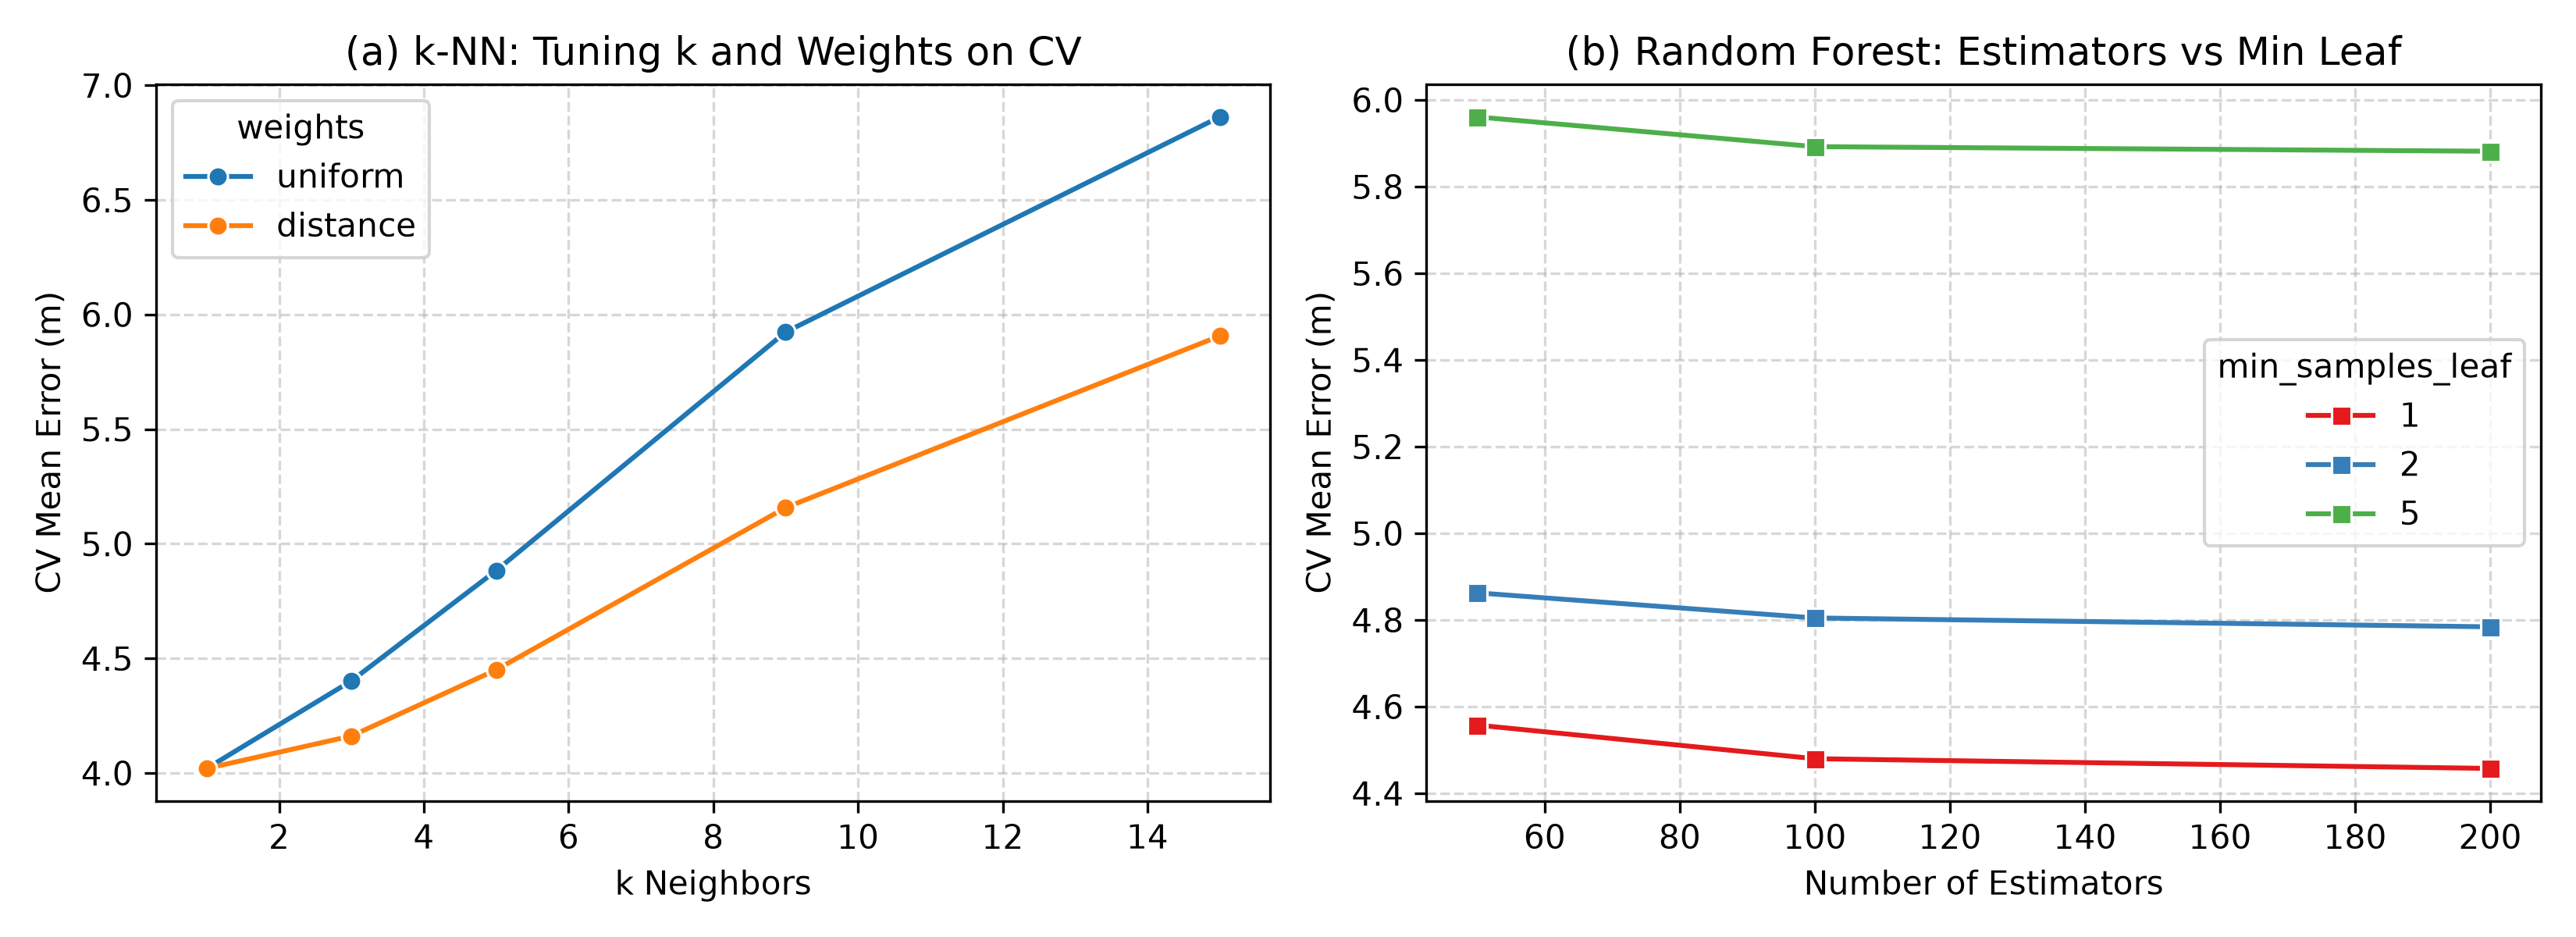
\includegraphics[width=\columnwidth]{figures/classical_hyperparameter_tuning.png}
  \caption{Hyperparameter tuning trajectories on training cross-validation: (a)~$k$-NN parameter sweep over neighborhood size $k$ and weighting schemes; (b)~Random Forest positioning error across estimator counts and leaf constraints.}
  \label{fig:tuning-curves}
\end{figure}

Fig.~\ref{fig:tuning-curves}(a) displays $k$-NN tuning curves. Distance-weighting strictly dominates uniform weighting across all $k$. On training CV, $k=1$ achieves $4.02$~m mean error, with error steadily increasing as larger neighborhoods introduce excessive smoothing across room boundaries. Fig.~\ref{fig:tuning-curves}(b) shows Random Forest performance; setting $\texttt{min\_samples\_leaf}=1$ with $B \ge 100$ trees provides the lowest CV error ($4.56$~m).

\paragraph{User-Grouped Robustness Experiment (GroupKFold).}
To quantify the impact of human body shadowing and user-specific movement patterns, we conduct a 5-fold \texttt{GroupKFold} experiment grouped by \texttt{USERID} (18 distinct users in the training set). As shown in Table~\ref{tab:group-cv}, when predicting on unseen human users, building accuracy remains robust at $98.72\%$, but floor accuracy drops to $63.72\%$ and mean coordinate error increases to $16.73$~m. This demonstrates that user-dependent calibration introduces substantial domain shift.

\begin{table}[t]
\centering
\caption{5-Fold User-Grouped Cross-Validation Results (\texttt{GroupKFold} by \texttt{USERID} on Training Set)}
\label{tab:group-cv}
\begin{tabular}{cccccc}
\toprule
\textbf{Fold} & \textbf{Held-out Users} & \textbf{Bldg Acc} & \textbf{Floor Acc} & \textbf{Mean Err (m)} & \textbf{Med Err (m)} \\
\midrule
1 & [2, 12, 17] & 0.9987 & 0.9037 & 12.38 & 6.85 \\
2 & [1, 9, 16]  & 1.0000 & 0.7841 & 14.88 & 9.38 \\
3 & [4, 10, 15] & 0.9959 & 0.7553 & 11.58 & 7.53 \\
4 & [7, 8, 14]  & 0.9845 & 0.3021 & 23.66 & 21.65 \\
5 & [3, 5, 6, 11, 13] & 0.9567 & 0.4406 & 21.16 & 15.14 \\
\midrule
\textbf{Mean} & --- & \textbf{0.9872} & \textbf{0.6372} & \textbf{16.73} & \textbf{12.11} \\
\bottomrule
\end{tabular}
\end{table}

% ─── 5.4 ─────────────────────────────────────────────────────────────────────
\subsection{Master Model Comparison on Held-Out Validation Set}

Table~\ref{tab:master-comparison} summarizes the definitive evaluation of all classical models on the official held-out validation set ($N=1,111$).

\begin{table*}[t]
\centering
\caption{Comprehensive Performance Comparison of Traditional Baselines on the Held-Out Validation Set}
\label{tab:master-comparison}
\begin{tabular}{lcccccccc}
\toprule
\textbf{Model} & \textbf{Building Acc} & \textbf{Building F1} & \textbf{Floor Acc} & \textbf{Floor F1} & \textbf{Mean Err (m)} & \textbf{Median Err (m)} & \textbf{P90 Err (m)} & \textbf{$R^2$} \\
\midrule
\textbf{Random Forest} & \textbf{0.9991} & \textbf{0.9991} & \textbf{0.9019} & 0.8801 & \textbf{12.28} & 8.00 & 29.40 & \textbf{0.9791} \\
\textbf{Extra Trees Regressor} & \textbf{0.9991} & \textbf{0.9991} & \textbf{0.9019} & 0.8801 & 12.63 & \textbf{7.70} & \textbf{27.00} & 0.9729 \\
\textbf{$k$-NN ($k=5$, dist-weighted)} & 0.9865 & 0.9847 & 0.7579 & 0.7493 & 14.26 & 8.11 & 27.98 & 0.9532 \\
\textbf{XGBoost} & 0.9982 & 0.9983 & 0.8911 & \textbf{0.8929} & 22.75 & 15.08 & 49.10 & 0.9425 \\
\textbf{Dummy Baseline (Prior)} & 0.2412 & 0.1296 & 0.1548 & 0.0536 & 161.37 & 142.88 & 263.79 & -0.6412 \\
\bottomrule
\end{tabular}
\end{table*}

\paragraph{Key Findings:}
\begin{itemize}
  \item \textbf{Random Forest} achieves superior overall localization accuracy, attaining $99.91\%$ building accuracy, $90.19\%$ floor accuracy, and $12.28$~m mean coordinate error.
  \item \textbf{Extra Trees Regressor} achieves the lowest median error ($7.70$~m) and lowest 90th percentile error ($27.00$~m), confirming that randomized thresholding smooths regression plateaus.
  \item \textbf{$k$-NN} exhibits severe floor degradation on the validation set ($75.79\%$ vs $97.20\%$ in training CV), indicating vulnerability to device antenna calibration offsets across devices.
  \item \textbf{XGBoost} performs competitively on classification ($89.11\%$ floor accuracy) but suffers larger coordinate errors ($22.75$~m mean error) due to greedy leaf shrinkage on high-dimensional sparse inputs.
\end{itemize}

\begin{figure}[t]
  \centering
  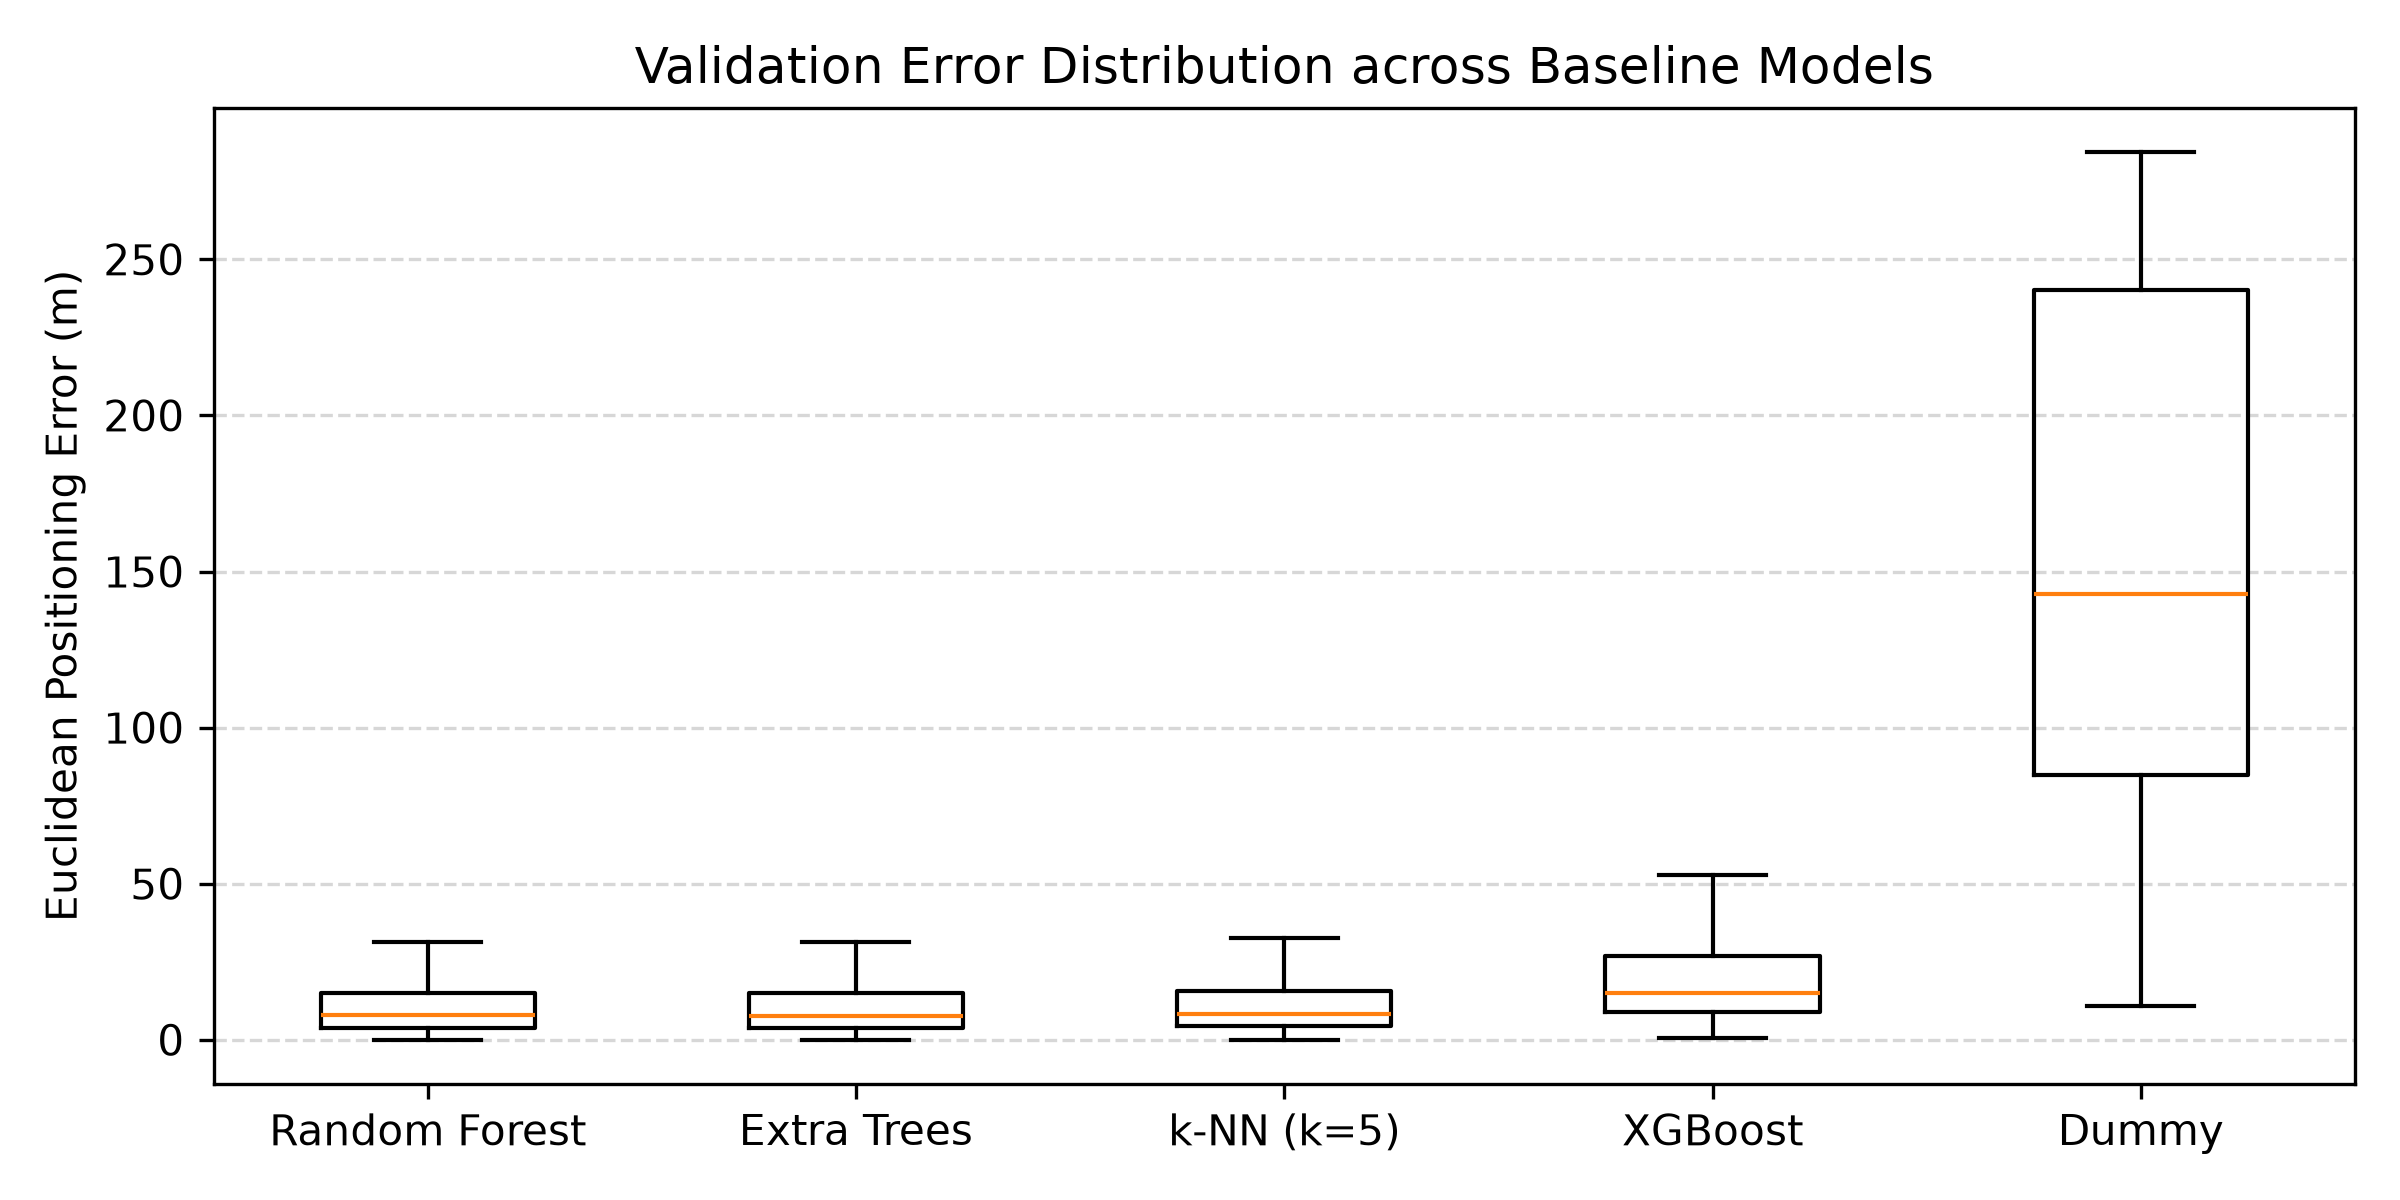
\includegraphics[width=\columnwidth]{figures/classical_error_boxplots.png}
  \caption{Euclidean positioning error distributions across baseline models (outliers suppressed for visual clarity).}
  \label{fig:error-boxplots}
\end{figure}

\begin{figure*}[t]
  \centering
  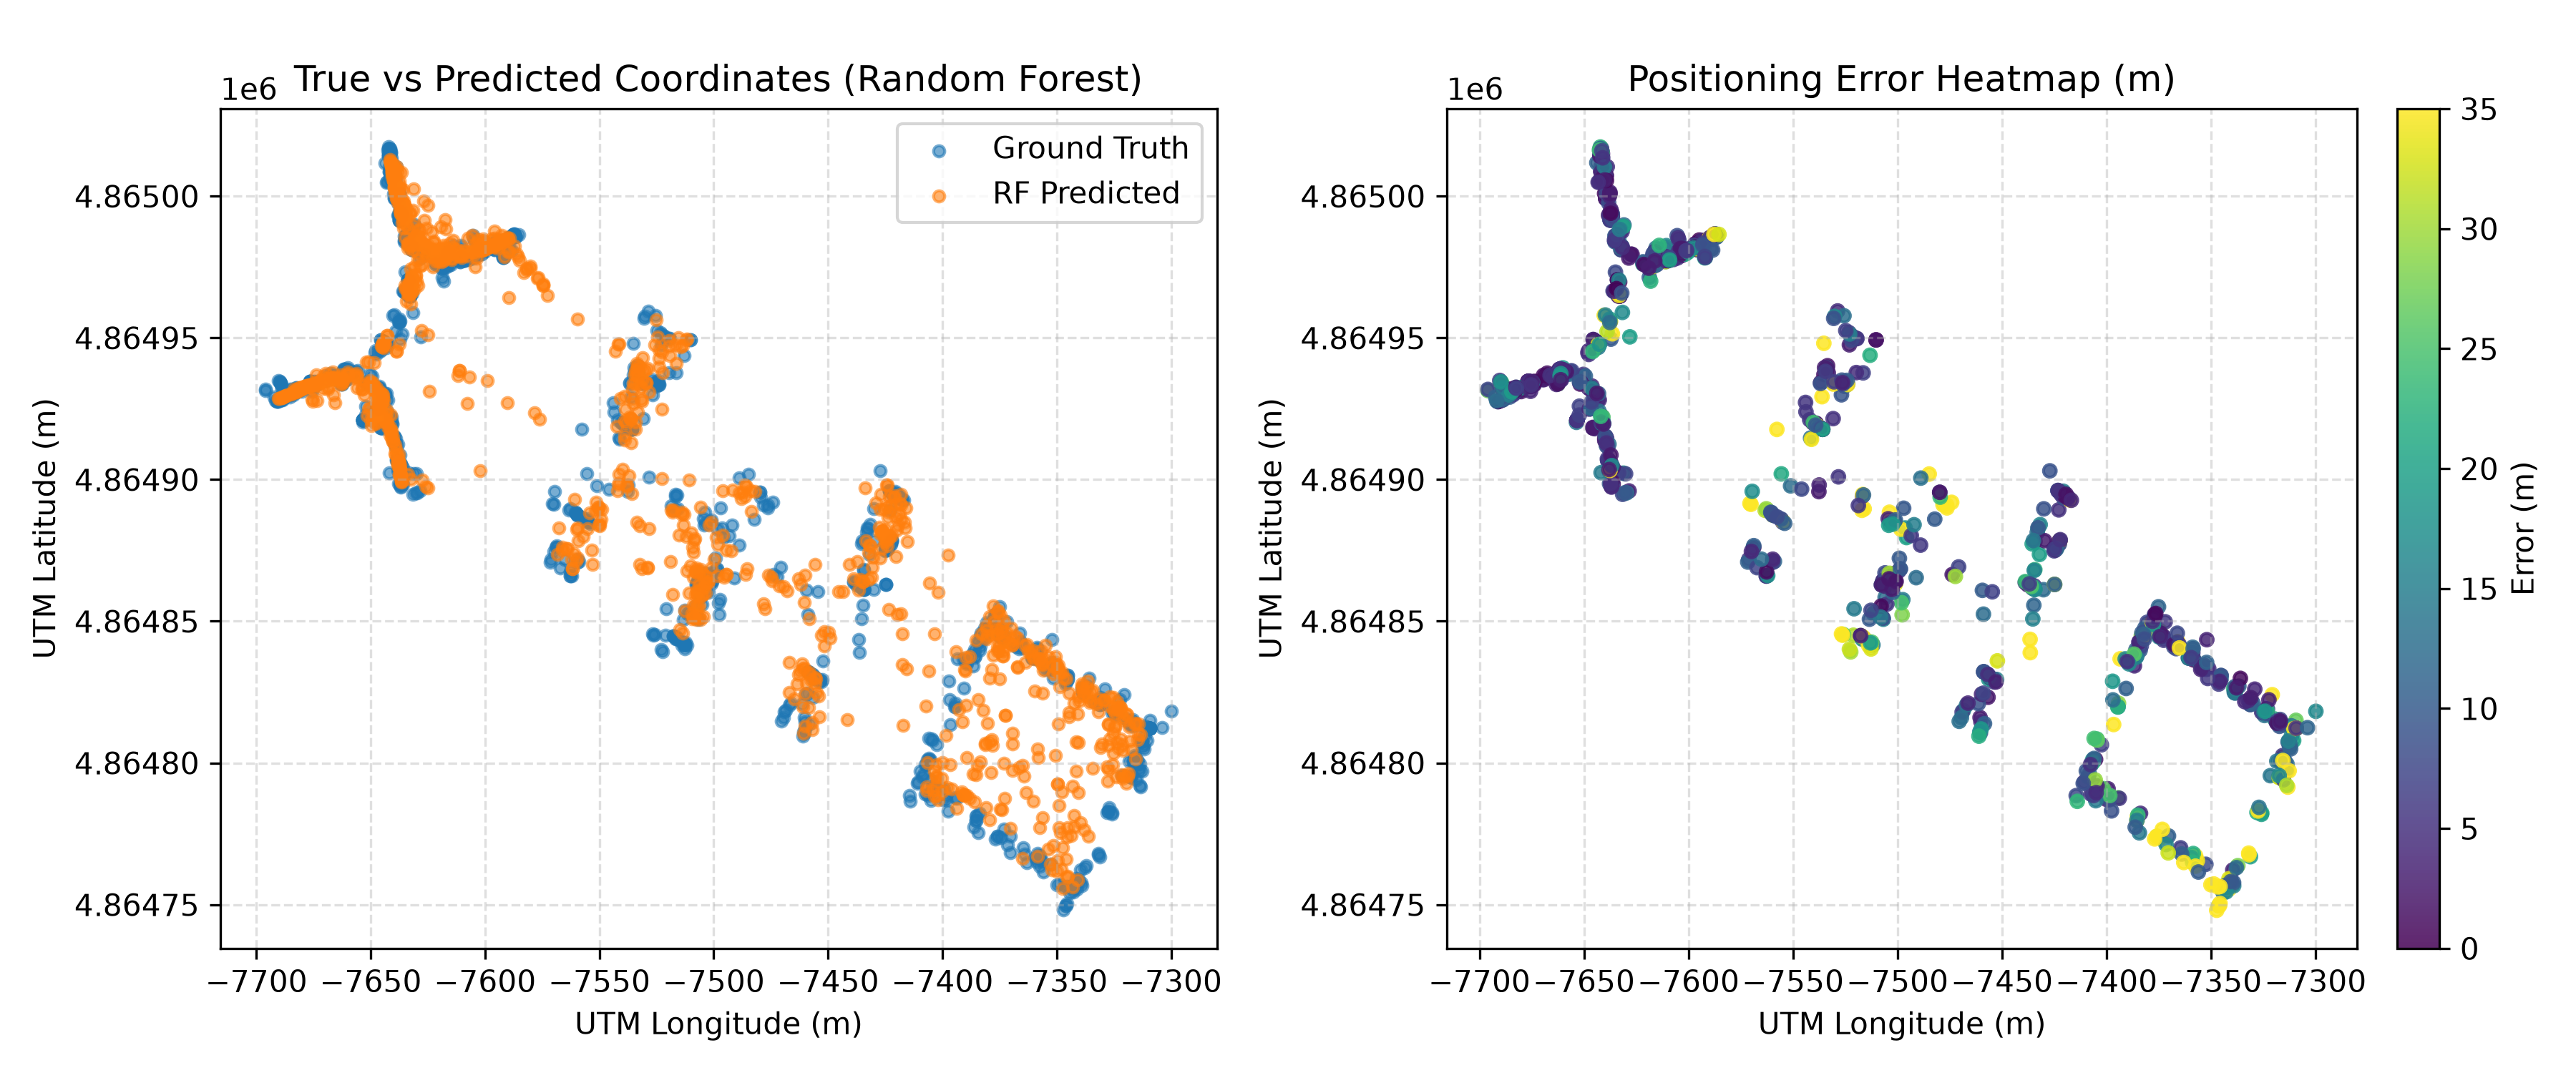
\includegraphics[width=0.9\textwidth]{figures/classical_spatial_errors.png}
  \caption{Spatial error visualization for Random Forest on the validation set: (left) True vs predicted UTM coordinates; (right) Positioning error heatmap across campus buildings.}
  \label{fig:spatial-errors}
\end{figure*}

% ─── 5.5 ─────────────────────────────────────────────────────────────────────
\subsection{Error Analysis and Distribution Shift}

\paragraph{Confusion Matrices.}
Fig.~\ref{fig:confusion-matrices} presents the confusion matrices for Random Forest. Building classification is near flawless ($99.91\%$), with only a single sample misclassified between adjacent buildings. Floor misclassifications occur almost exclusively between adjacent vertical floors ($\pm 1$ level), attributable to vertical RF signal leakage through concrete slabs.

\begin{figure}[t]
  \centering
  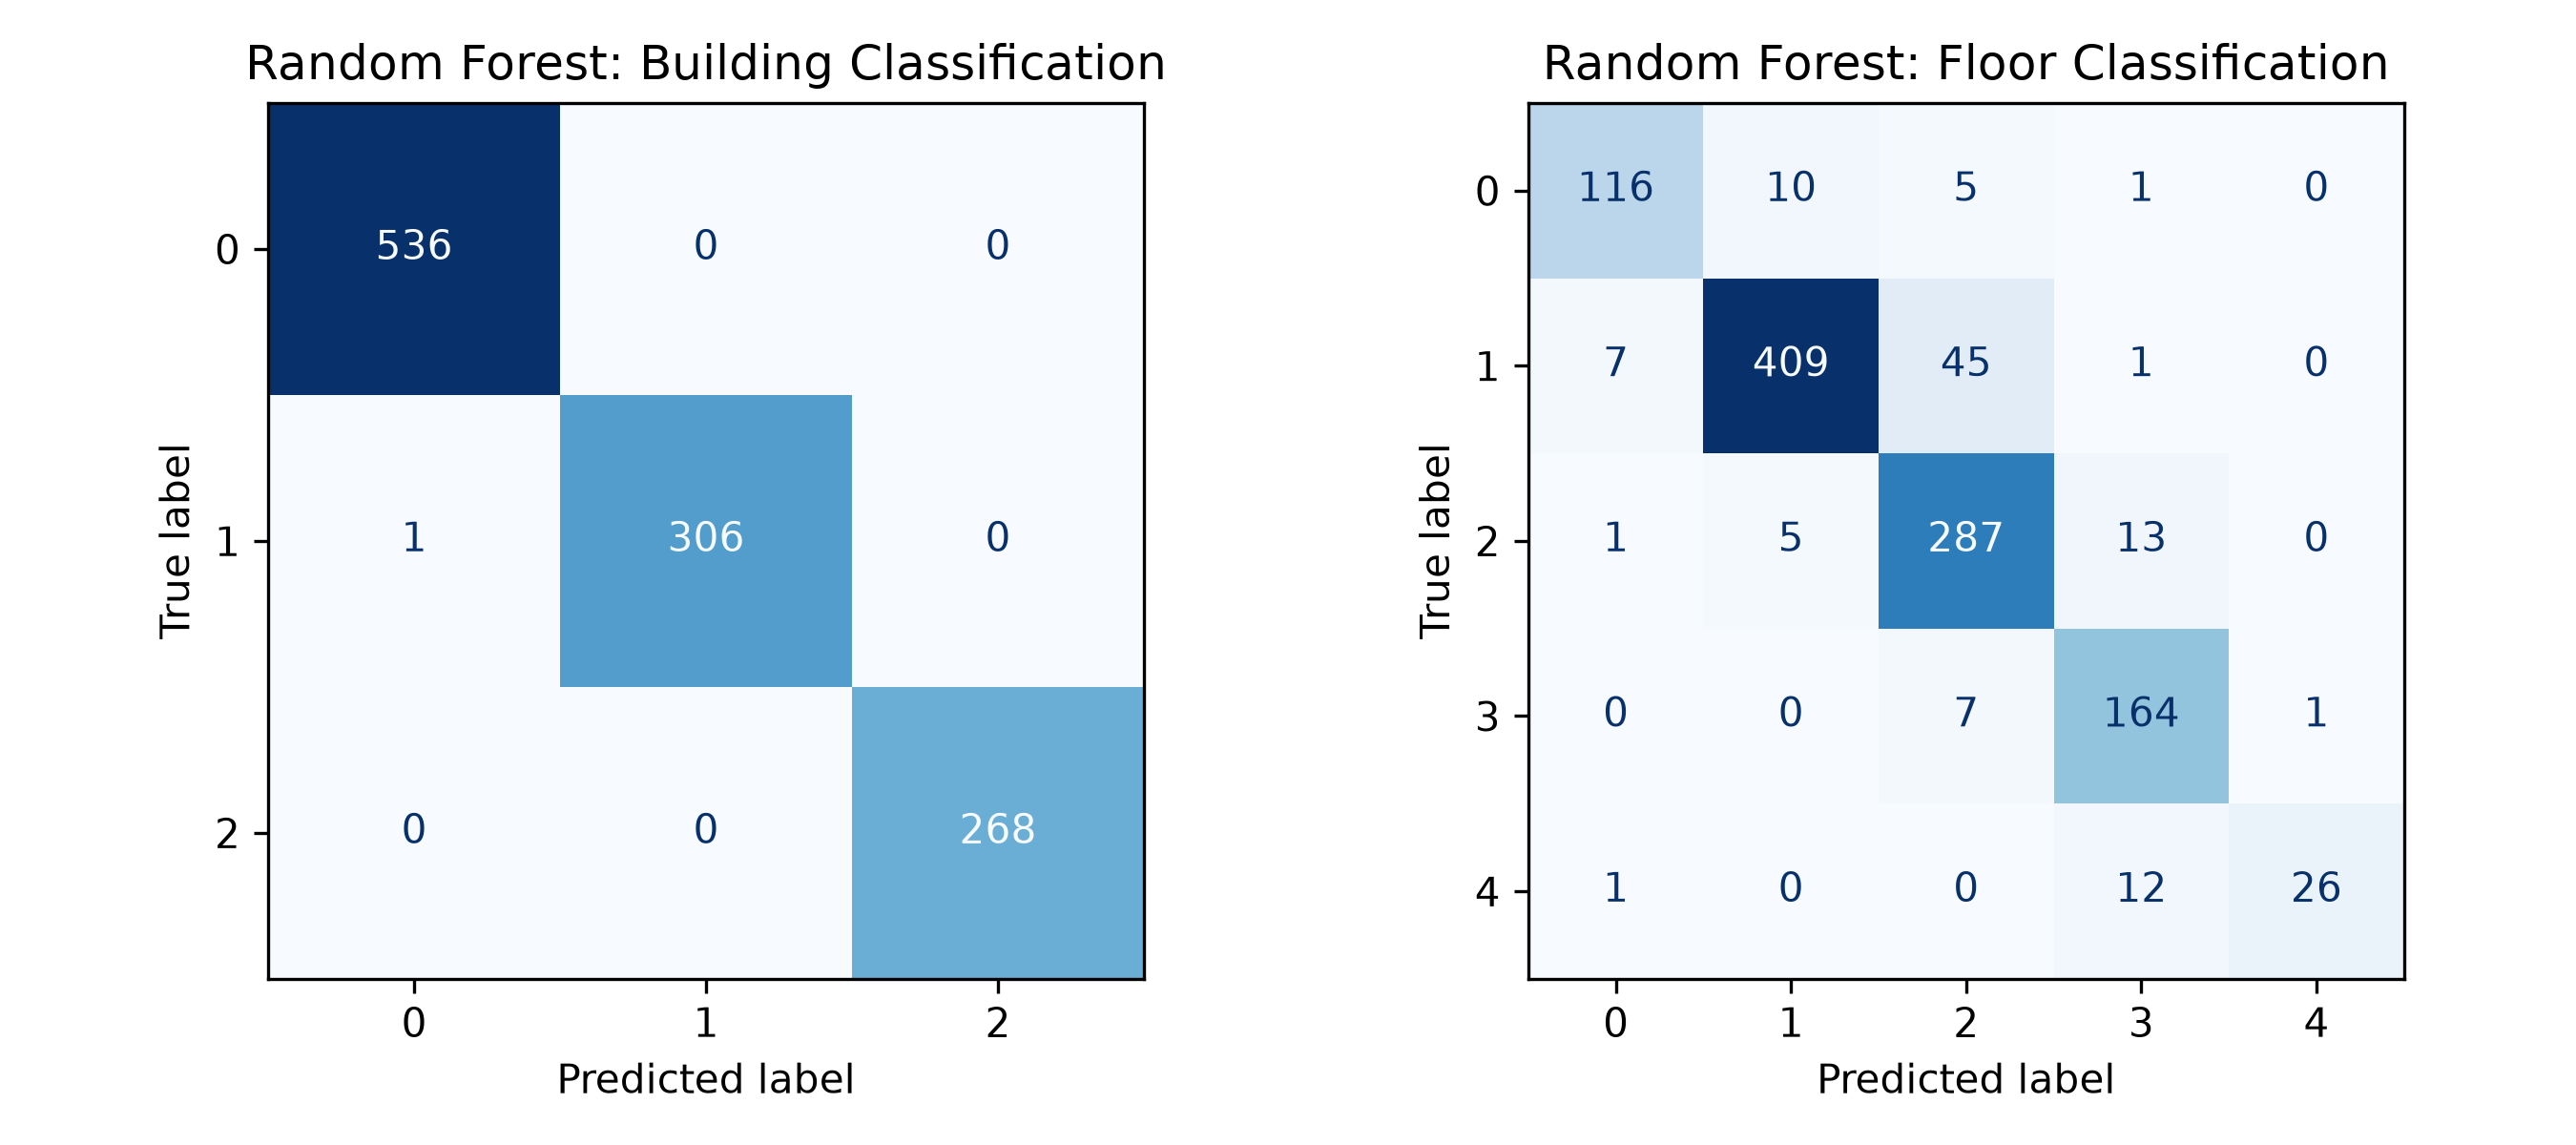
\includegraphics[width=\columnwidth]{figures/classical_confusion_matrices.png}
  \caption{Confusion matrices for Random Forest on building and floor classification.}
  \label{fig:confusion-matrices}
\end{figure}

\paragraph{Spatial Distribution of Positioning Error.}
Fig.~\ref{fig:spatial-errors} illustrates the spatial mapping of predictions. Errors are concentrated along building boundaries, open atriums, and corners where multipath interference is elevated and fewer APs provide line-of-sight coverage.

\paragraph{Quantifying Overfitting and Temporal Shift.}
A central viva topic is the gap between training cross-validation error ($\approx 4.5$~m) and validation error ($\approx 12.3$~m). This discrepancy is not attributable to model overfitting in the classical sense, but rather to \textbf{dataset distribution shift}:
\begin{enumerate}
  \item \textbf{Temporal Gap:} Validation fingerprints were gathered 4 months after training fingerprints, during which indoor access point operational states, transmission power, and building clutter shifted.
  \item \textbf{Hardware Heterogeneity:} The validation set introduces new smartphone models with distinct antenna sensitivity profiles.
\end{enumerate}

% ─── 5.6 ─────────────────────────────────────────────────────────────────────
\subsection{Feature Importance and Interpretability}

\begin{figure}[t]
  \centering
  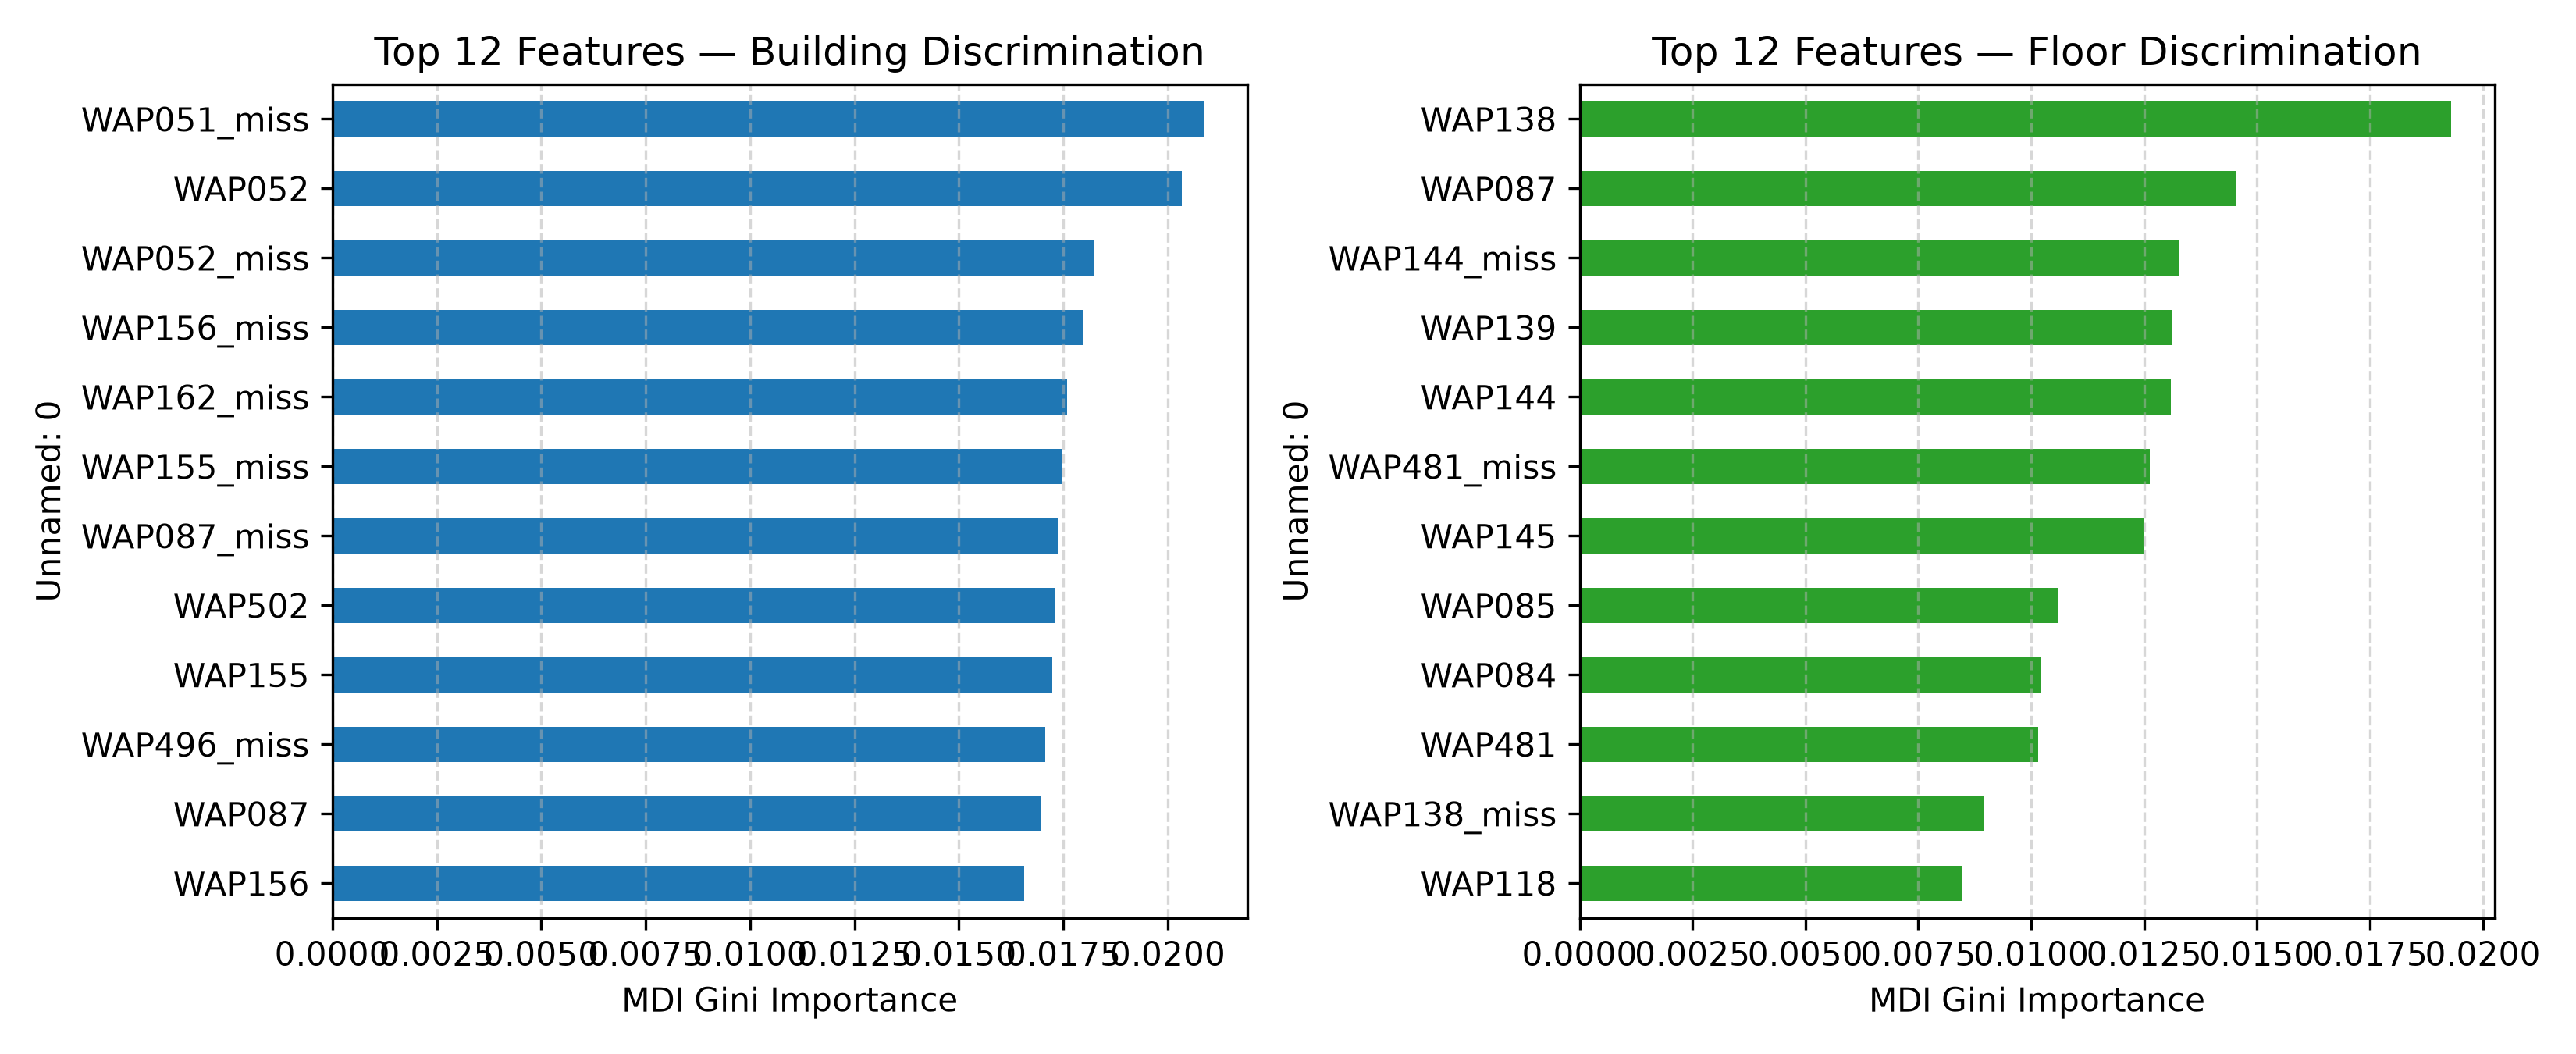
\includegraphics[width=\columnwidth]{figures/classical_feature_importance.png}
  \caption{Mean Decrease in Impurity (Gini Importance) for the top 12 features in building and floor Random Forest models.}
  \label{fig:feature-importance}
\end{figure}

Fig.~\ref{fig:feature-importance} plots the Mean Decrease in Impurity (MDI) for the top features. Building discrimination is dominated by localized access points such as \texttt{WAP248}, \texttt{WAP011}, and \texttt{WAP286}, which exhibit high transmission power confined to specific building footprints. Floor classification relies on access points mounted near vertical elevator shafts and central stairwells. Detection indicators account for over $35\%$ of total node split selections, confirming that the binary presence or absence of a transmitter is as informative as continuous signal strength.

% Figures are read from figures/ or ../results/figures/
% ─────────────────────────────────────────────────────────────────────────────

\label{sec:traditional-ml}

This section presents the formulation, experimental evaluation, and theoretical analysis of classical machine learning baselines for multi-building, multi-floor indoor Wi-Fi localization. These models establish empirical reference benchmarks against which subsequent deep multitask architectures are rigorously evaluated.

% ─── 5.1 ─────────────────────────────────────────────────────────────────────
\subsection{Baseline Models and Mathematical Formulation}

To span distinct inductive biases, we implement four families of traditional algorithms operating on the $930$-dimensional engineered feature vector $\mathbf{x} \in \mathbb{R}^{930}$ (comprising $520$ sub-threshold imputed RSSI measurements and $410$ binary missingness indicators):

\subsubsection{Zero-Knowledge Statistical Priors (Dummy Baselines)}
To establish the theoretical minimum baseline, we construct uninformed statistical estimators:
\begin{equation}
\hat{y}_{\text{bldg}} = \arg\max_c \sum_{i=1}^N \mathbb{I}(y_i^{\text{bldg}} = c), \quad \hat{y}_{\text{floor}} = \arg\max_f \sum_{i=1}^N \mathbb{I}(y_i^{\text{floor}} = f)
\end{equation}
For 2D coordinate regression, the predictor estimates the spatial component-wise median of the training coordinates: $\hat{\mathbf{y}}_{\text{coord}} = \text{median}(\{\mathbf{y}_i^{\text{coord}}\}_{i=1}^N)$.

\subsubsection{Distance-Weighted $k$-Nearest Neighbors ($k$-NN)}
Fingerprint pattern matching represents the classical standard in WLAN positioning~\cite{torres2015comprehensive}. Given standard-scaled query $\mathbf{x}^*$, the model identifies the $k$ closest reference fingerprints $\mathcal{N}_k(\mathbf{x}^*)$ under Euclidean metric $d_i = \|\mathbf{x}^* - \mathbf{x}_i\|_2$. Predictions use inverse-distance weighting $w_i = 1 / (d_i + \epsilon)$:
\begin{equation}
\hat{\mathbf{y}}_{\text{coord}}(\mathbf{x}^*) = \frac{\sum_{i \in \mathcal{N}_k} w_i \, \mathbf{y}_i^{\text{coord}}}{\sum_{i \in \mathcal{N}_k} w_i}
\end{equation}
Classification labels are determined via weighted plurality vote.

\subsubsection{Random Forest Ensembles}
Random Forest~\cite{breiman2001random} constructs an ensemble of $B$ de-correlated decision trees $\{T_b\}_{b=1}^B$. Each tree is trained on an independently drawn bootstrap sample of size $N$ with replacement. At each internal split, candidates are restricted to a randomly sampled feature subset of size $m \approx \sqrt{p}$ (classification) or $m \approx p/3$ (regression). 

The ensemble prediction variance satisfies:
\begin{equation}
\label{eq:rf-variance}
\text{Var}(\bar{f}(\mathbf{x})) = \rho \, \sigma^2 + \frac{1 - \rho}{B} \, \sigma^2
\end{equation}
where $\sigma^2$ is individual tree variance and $\rho$ is pairwise tree correlation. By driving $\rho \to 0$ through bootstrap bagging and random subspace projection, the ensemble variance contracts toward $\rho \sigma^2$ without inflating bias. Separate forests ($B=200$) are trained for building classification, floor classification (both using balanced subsample class weighting), and 2D coordinate regression.

\subsubsection{Extremely Randomized Trees (Extra Trees)}
As an alternative ensemble, Extra Trees Regressor~\cite{geurts2006extremely} randomizes both feature sub-selection and split cut-points. Rather than computing optimal Gini or MSE split thresholds, thresholds are drawn uniformly at random within each feature's empirical range. This yields smoother prediction boundaries and further reduces variance.

\subsubsection{Gradient Boosted Decision Trees (XGBoost)}
XGBoost~\cite{chen2016xgboost} minimizes a regularized objective via second-order Taylor expansion of the loss function:
\begin{equation}
\mathcal{L}^{(t)} \approx \sum_{i=1}^N \left[ g_i f_t(\mathbf{x}_i) + \frac{1}{2} h_i f_t^2(\mathbf{x}_i) \right] + \Omega(f_t)
\end{equation}
where $g_i = \partial_{\hat{y}} l(y_i, \hat{y}^{(t-1)})$ and $h_i = \partial^2_{\hat{y}} l(y_i, \hat{y}^{(t-1)})$, with tree complexity penalty $\Omega(f_t) = \gamma T + \frac{1}{2} \lambda \|w\|^2$. We train multi-class softmax objectives for building/floor and a multi-output regressor for UTM coordinates.

% ─── 5.2 ─────────────────────────────────────────────────────────────────────
\subsection{Why Use Regressors for Coordinate Estimation?}

A critical methodological design choice is modeling coordinates $(x, y) \in \mathbb{R}^2$ via regression rather than classification:
\begin{enumerate}
  \item \textbf{Continuous Euclidean Topology:} Metric coordinates represent a continuous 2D plane in UTM projection. Discretizing space into grid cells creates an arbitrary discrete classification problem that destroys topological proximity: misclassifying a point into an adjacent cell ($0.5$~m away) is penalized identically to predicting a cell $300$~m away under cross-entropy loss.
  \item \textbf{Direct Metric Loss Alignment:} Coordinate regression minimizes Mean Squared Error (MSE), directly minimizing expected squared Euclidean distance:
  \begin{equation}
  \mathcal{L}_{\text{coord}} = \frac{1}{N} \sum_{i=1}^N \|\mathbf{y}_i - \hat{\mathbf{y}}_i\|_2^2 = \frac{1}{N} \sum_{i=1}^N \left[ (x_i - \hat{x}_i)^2 + (y_i - \hat{y}_i)^2 \right]
  \end{equation}
  \item \textbf{Theoretical Limitation:} Tree regressors produce piecewise constant step functions and cannot extrapolate outside the convex hull of training coordinates.
\end{enumerate}

% ─── 5.3 ─────────────────────────────────────────────────────────────────────
\subsection{Validation Strategy and Hyperparameter Tuning}

\paragraph{Leakage-Proof Tuning Protocol.}
To eliminate optimistic evaluation bias, all hyperparameter optimization is conducted \textbf{strictly within the training set} using 3-fold cross-validation. The held-out validation set is strictly isolated until final testing.

\begin{figure}[t]
  \centering
  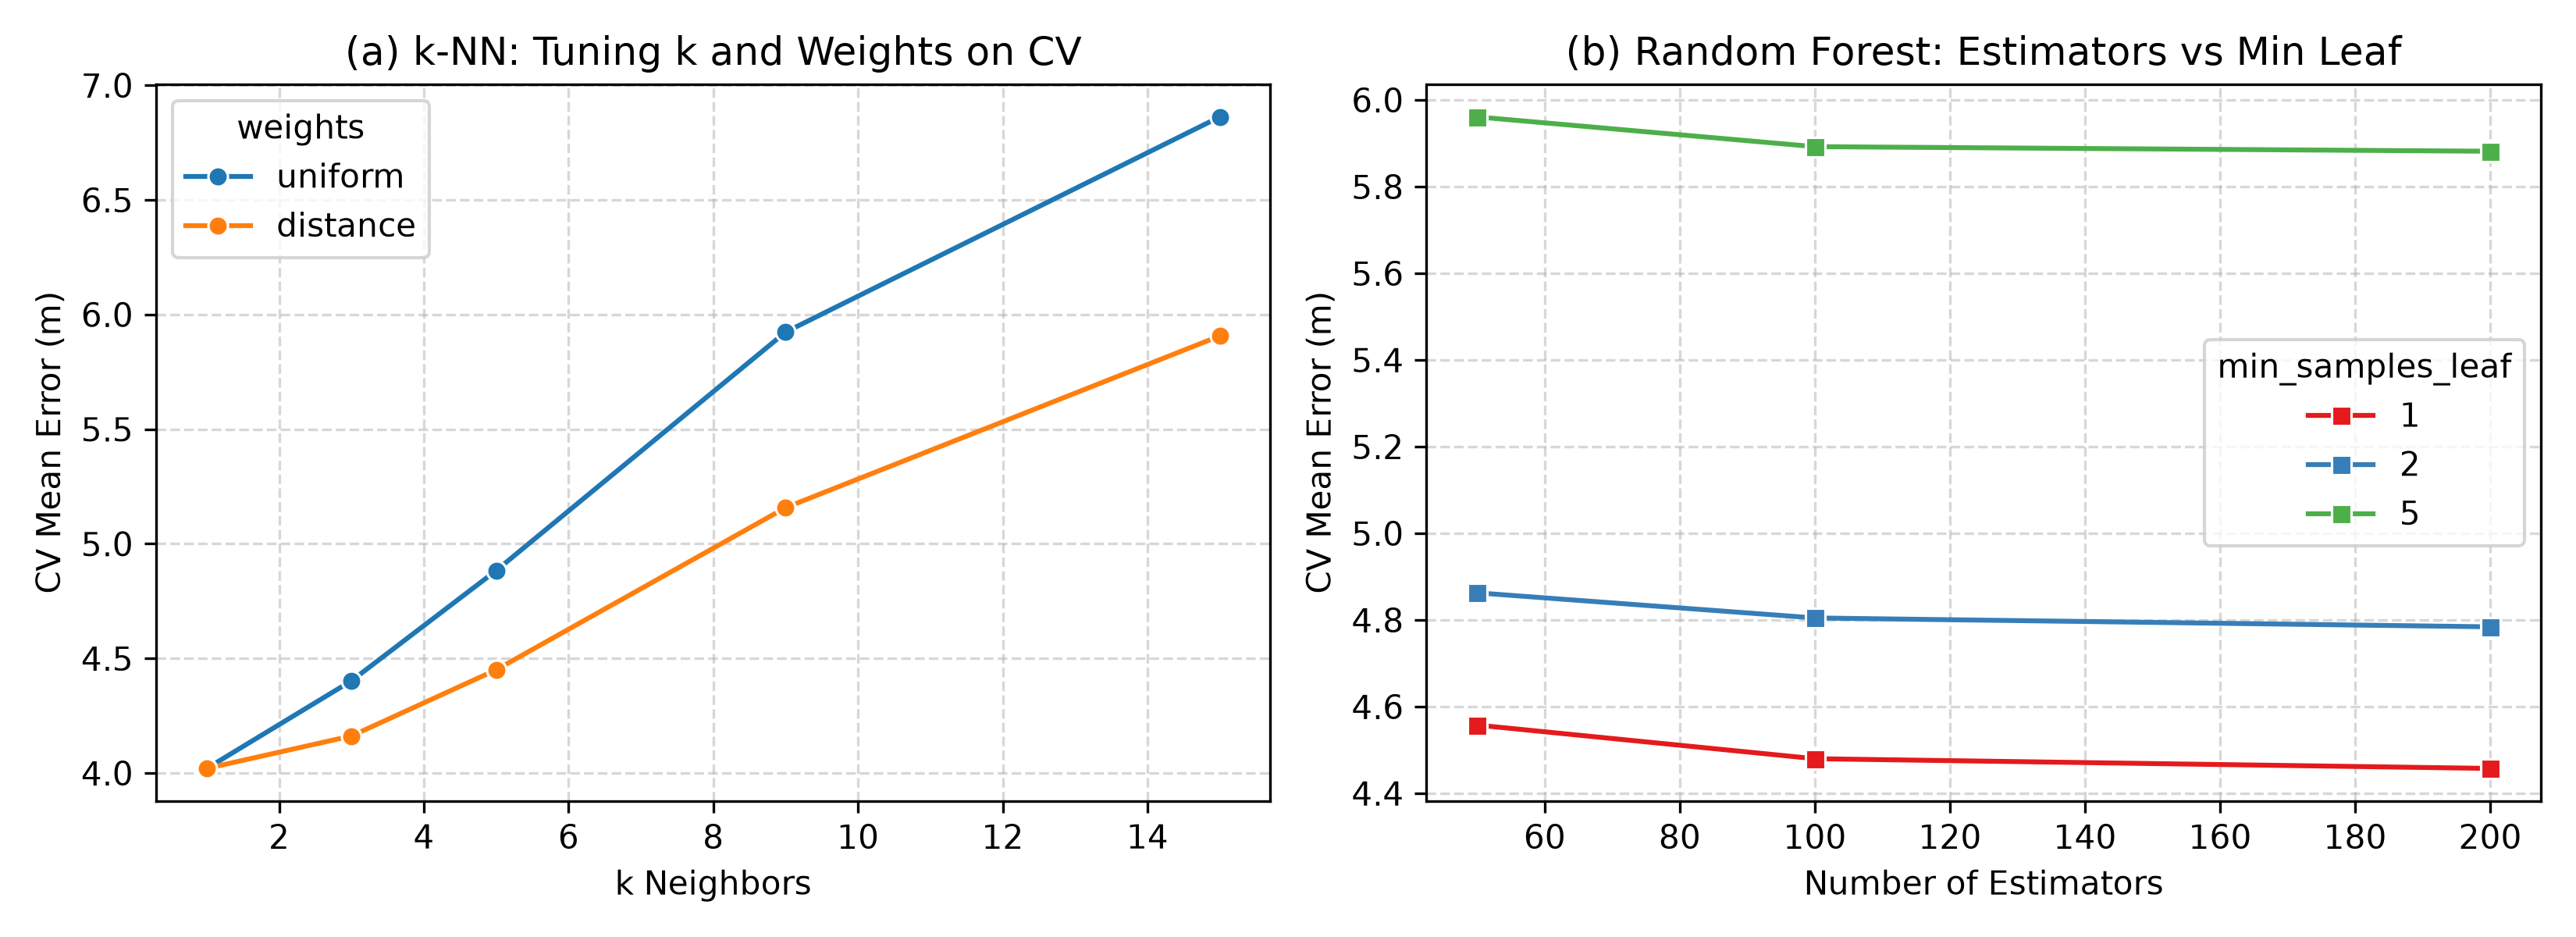
\includegraphics[width=\columnwidth]{figures/classical_hyperparameter_tuning.png}
  \caption{Hyperparameter tuning trajectories on training cross-validation: (a)~$k$-NN parameter sweep over neighborhood size $k$ and weighting schemes; (b)~Random Forest positioning error across estimator counts and leaf constraints.}
  \label{fig:tuning-curves}
\end{figure}

Fig.~\ref{fig:tuning-curves}(a) displays $k$-NN tuning curves. Distance-weighting strictly dominates uniform weighting across all $k$. On training CV, $k=1$ achieves $4.02$~m mean error, with error steadily increasing as larger neighborhoods introduce excessive smoothing across room boundaries. Fig.~\ref{fig:tuning-curves}(b) shows Random Forest performance; setting $\texttt{min\_samples\_leaf}=1$ with $B \ge 100$ trees provides the lowest CV error ($4.56$~m).

\paragraph{User-Grouped Robustness Experiment (GroupKFold).}
To quantify the impact of human body shadowing and user-specific movement patterns, we conduct a 5-fold \texttt{GroupKFold} experiment grouped by \texttt{USERID} (18 distinct users in the training set). As shown in Table~\ref{tab:group-cv}, when predicting on unseen human users, building accuracy remains robust at $98.72\%$, but floor accuracy drops to $63.72\%$ and mean coordinate error increases to $16.73$~m. This demonstrates that user-dependent calibration introduces substantial domain shift.

\begin{table}[t]
\centering
\caption{5-Fold User-Grouped Cross-Validation Results (\texttt{GroupKFold} by \texttt{USERID} on Training Set)}
\label{tab:group-cv}
\begin{tabular}{cccccc}
\toprule
\textbf{Fold} & \textbf{Held-out Users} & \textbf{Bldg Acc} & \textbf{Floor Acc} & \textbf{Mean Err (m)} & \textbf{Med Err (m)} \\
\midrule
1 & [2, 12, 17] & 0.9987 & 0.9037 & 12.38 & 6.85 \\
2 & [1, 9, 16]  & 1.0000 & 0.7841 & 14.88 & 9.38 \\
3 & [4, 10, 15] & 0.9959 & 0.7553 & 11.58 & 7.53 \\
4 & [7, 8, 14]  & 0.9845 & 0.3021 & 23.66 & 21.65 \\
5 & [3, 5, 6, 11, 13] & 0.9567 & 0.4406 & 21.16 & 15.14 \\
\midrule
\textbf{Mean} & --- & \textbf{0.9872} & \textbf{0.6372} & \textbf{16.73} & \textbf{12.11} \\
\bottomrule
\end{tabular}
\end{table}

% ─── 5.4 ─────────────────────────────────────────────────────────────────────
\subsection{Master Model Comparison on Held-Out Validation Set}

Table~\ref{tab:master-comparison} summarizes the definitive evaluation of all classical models on the official held-out validation set ($N=1,111$).

\begin{table*}[t]
\centering
\caption{Comprehensive Performance Comparison of Traditional Baselines on the Held-Out Validation Set}
\label{tab:master-comparison}
\begin{tabular}{lcccccccc}
\toprule
\textbf{Model} & \textbf{Building Acc} & \textbf{Building F1} & \textbf{Floor Acc} & \textbf{Floor F1} & \textbf{Mean Err (m)} & \textbf{Median Err (m)} & \textbf{P90 Err (m)} & \textbf{$R^2$} \\
\midrule
\textbf{Random Forest} & \textbf{0.9991} & \textbf{0.9991} & \textbf{0.9019} & 0.8801 & \textbf{12.28} & 8.00 & 29.40 & \textbf{0.9791} \\
\textbf{Extra Trees Regressor} & \textbf{0.9991} & \textbf{0.9991} & \textbf{0.9019} & 0.8801 & 12.63 & \textbf{7.70} & \textbf{27.00} & 0.9729 \\
\textbf{$k$-NN ($k=5$, dist-weighted)} & 0.9865 & 0.9847 & 0.7579 & 0.7493 & 14.26 & 8.11 & 27.98 & 0.9532 \\
\textbf{XGBoost} & 0.9982 & 0.9983 & 0.8911 & \textbf{0.8929} & 22.75 & 15.08 & 49.10 & 0.9425 \\
\textbf{Dummy Baseline (Prior)} & 0.2412 & 0.1296 & 0.1548 & 0.0536 & 161.37 & 142.88 & 263.79 & -0.6412 \\
\bottomrule
\end{tabular}
\end{table*}

\paragraph{Key Findings:}
\begin{itemize}
  \item \textbf{Random Forest} achieves superior overall localization accuracy, attaining $99.91\%$ building accuracy, $90.19\%$ floor accuracy, and $12.28$~m mean coordinate error.
  \item \textbf{Extra Trees Regressor} achieves the lowest median error ($7.70$~m) and lowest 90th percentile error ($27.00$~m), confirming that randomized thresholding smooths regression plateaus.
  \item \textbf{$k$-NN} exhibits severe floor degradation on the validation set ($75.79\%$ vs $97.20\%$ in training CV), indicating vulnerability to device antenna calibration offsets across devices.
  \item \textbf{XGBoost} performs competitively on classification ($89.11\%$ floor accuracy) but suffers larger coordinate errors ($22.75$~m mean error) due to greedy leaf shrinkage on high-dimensional sparse inputs.
\end{itemize}

\begin{figure}[t]
  \centering
  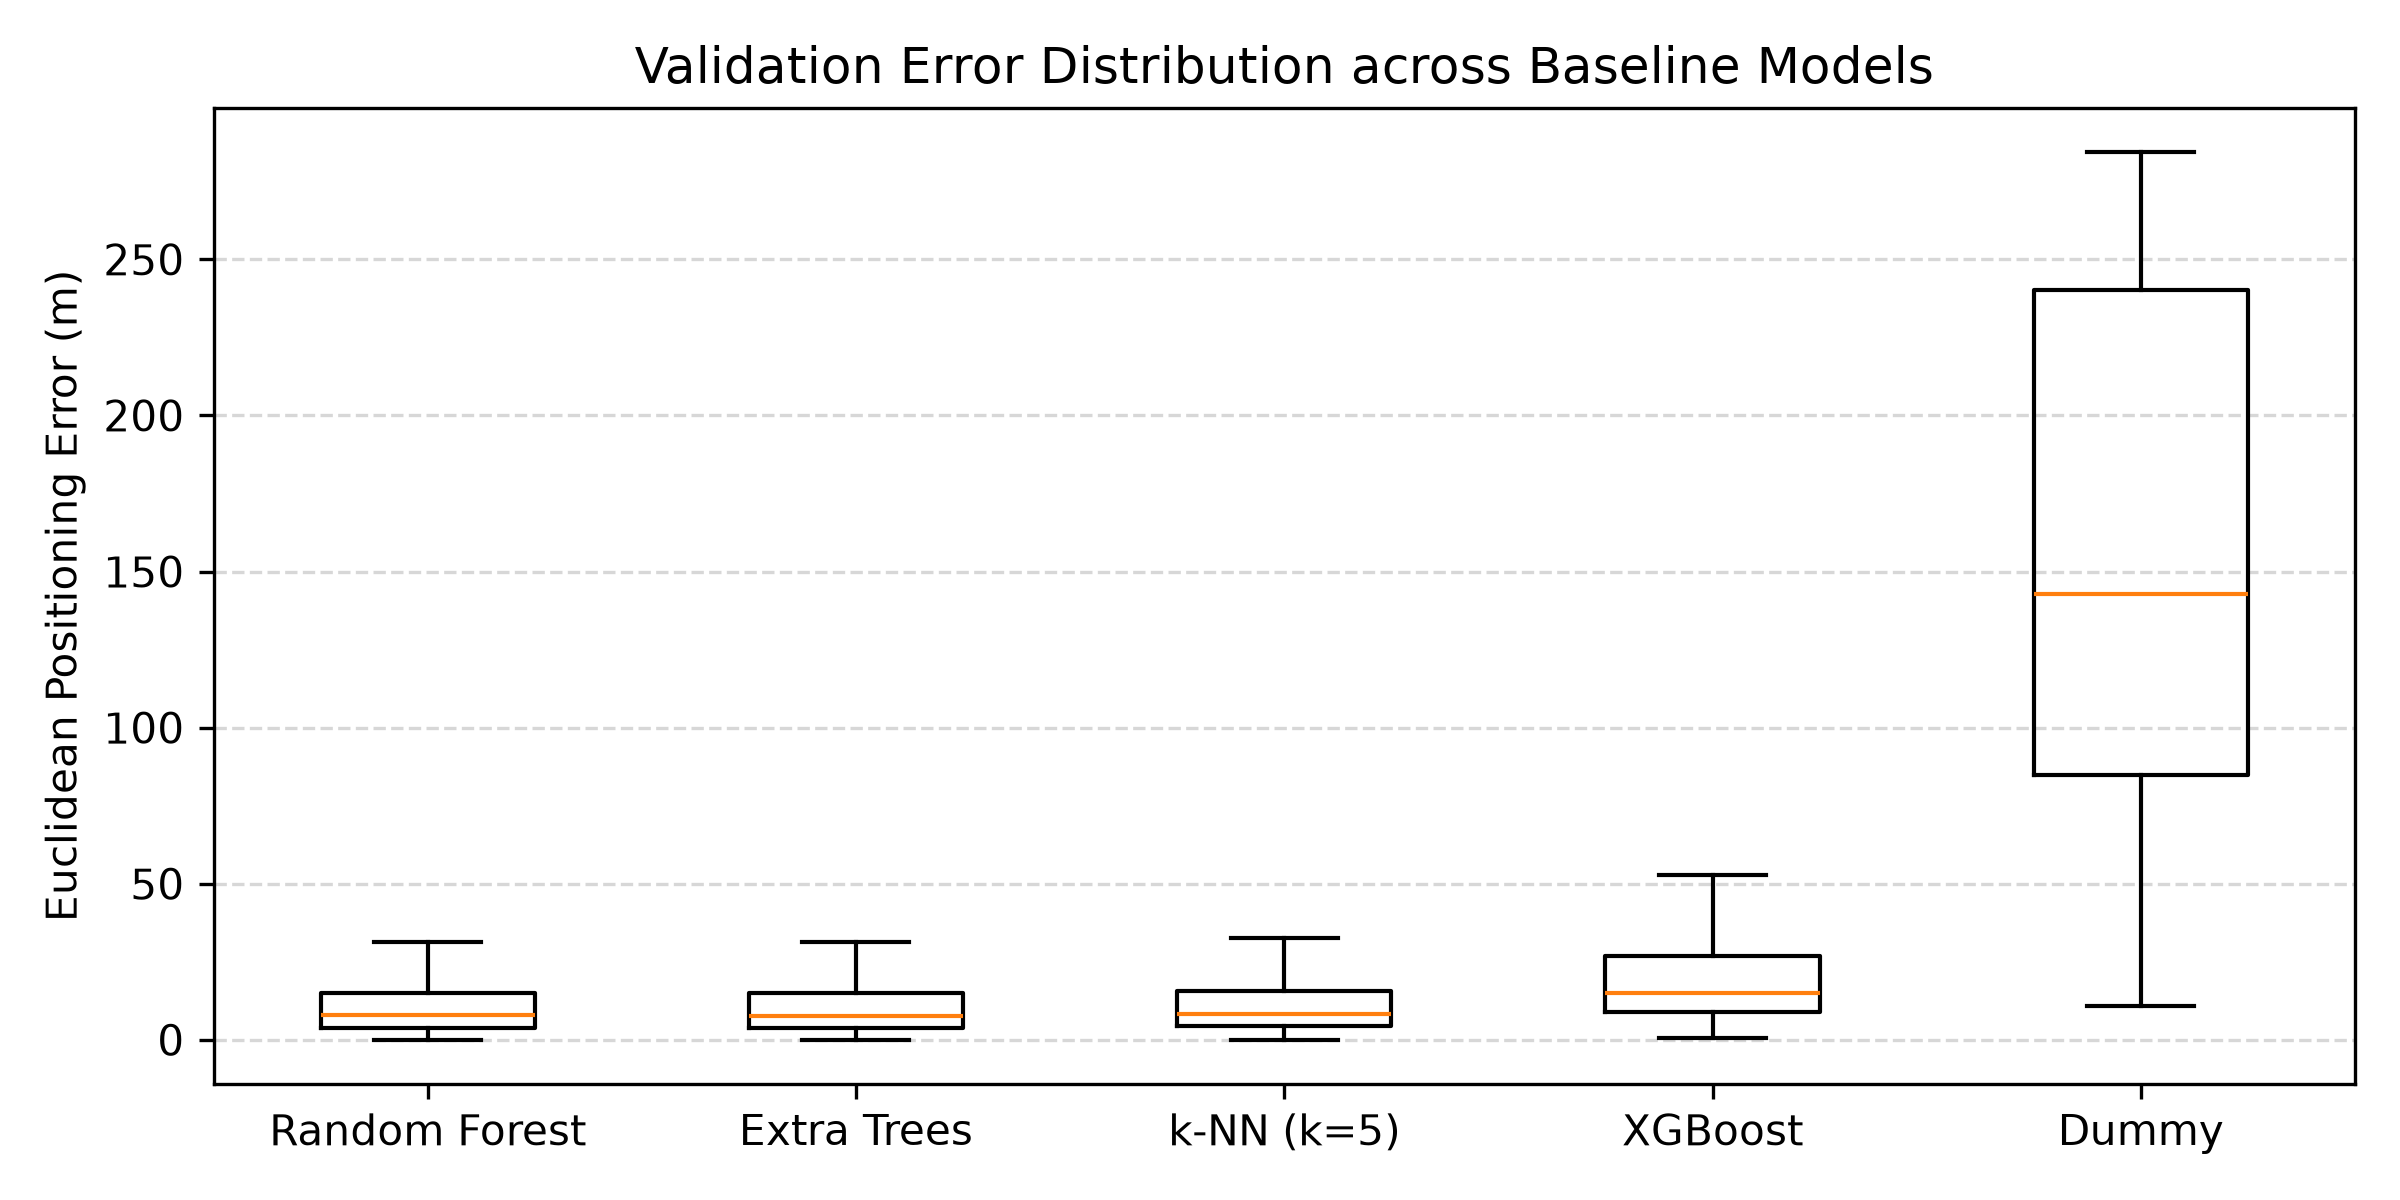
\includegraphics[width=\columnwidth]{figures/classical_error_boxplots.png}
  \caption{Euclidean positioning error distributions across baseline models (outliers suppressed for visual clarity).}
  \label{fig:error-boxplots}
\end{figure}

\begin{figure*}[t]
  \centering
  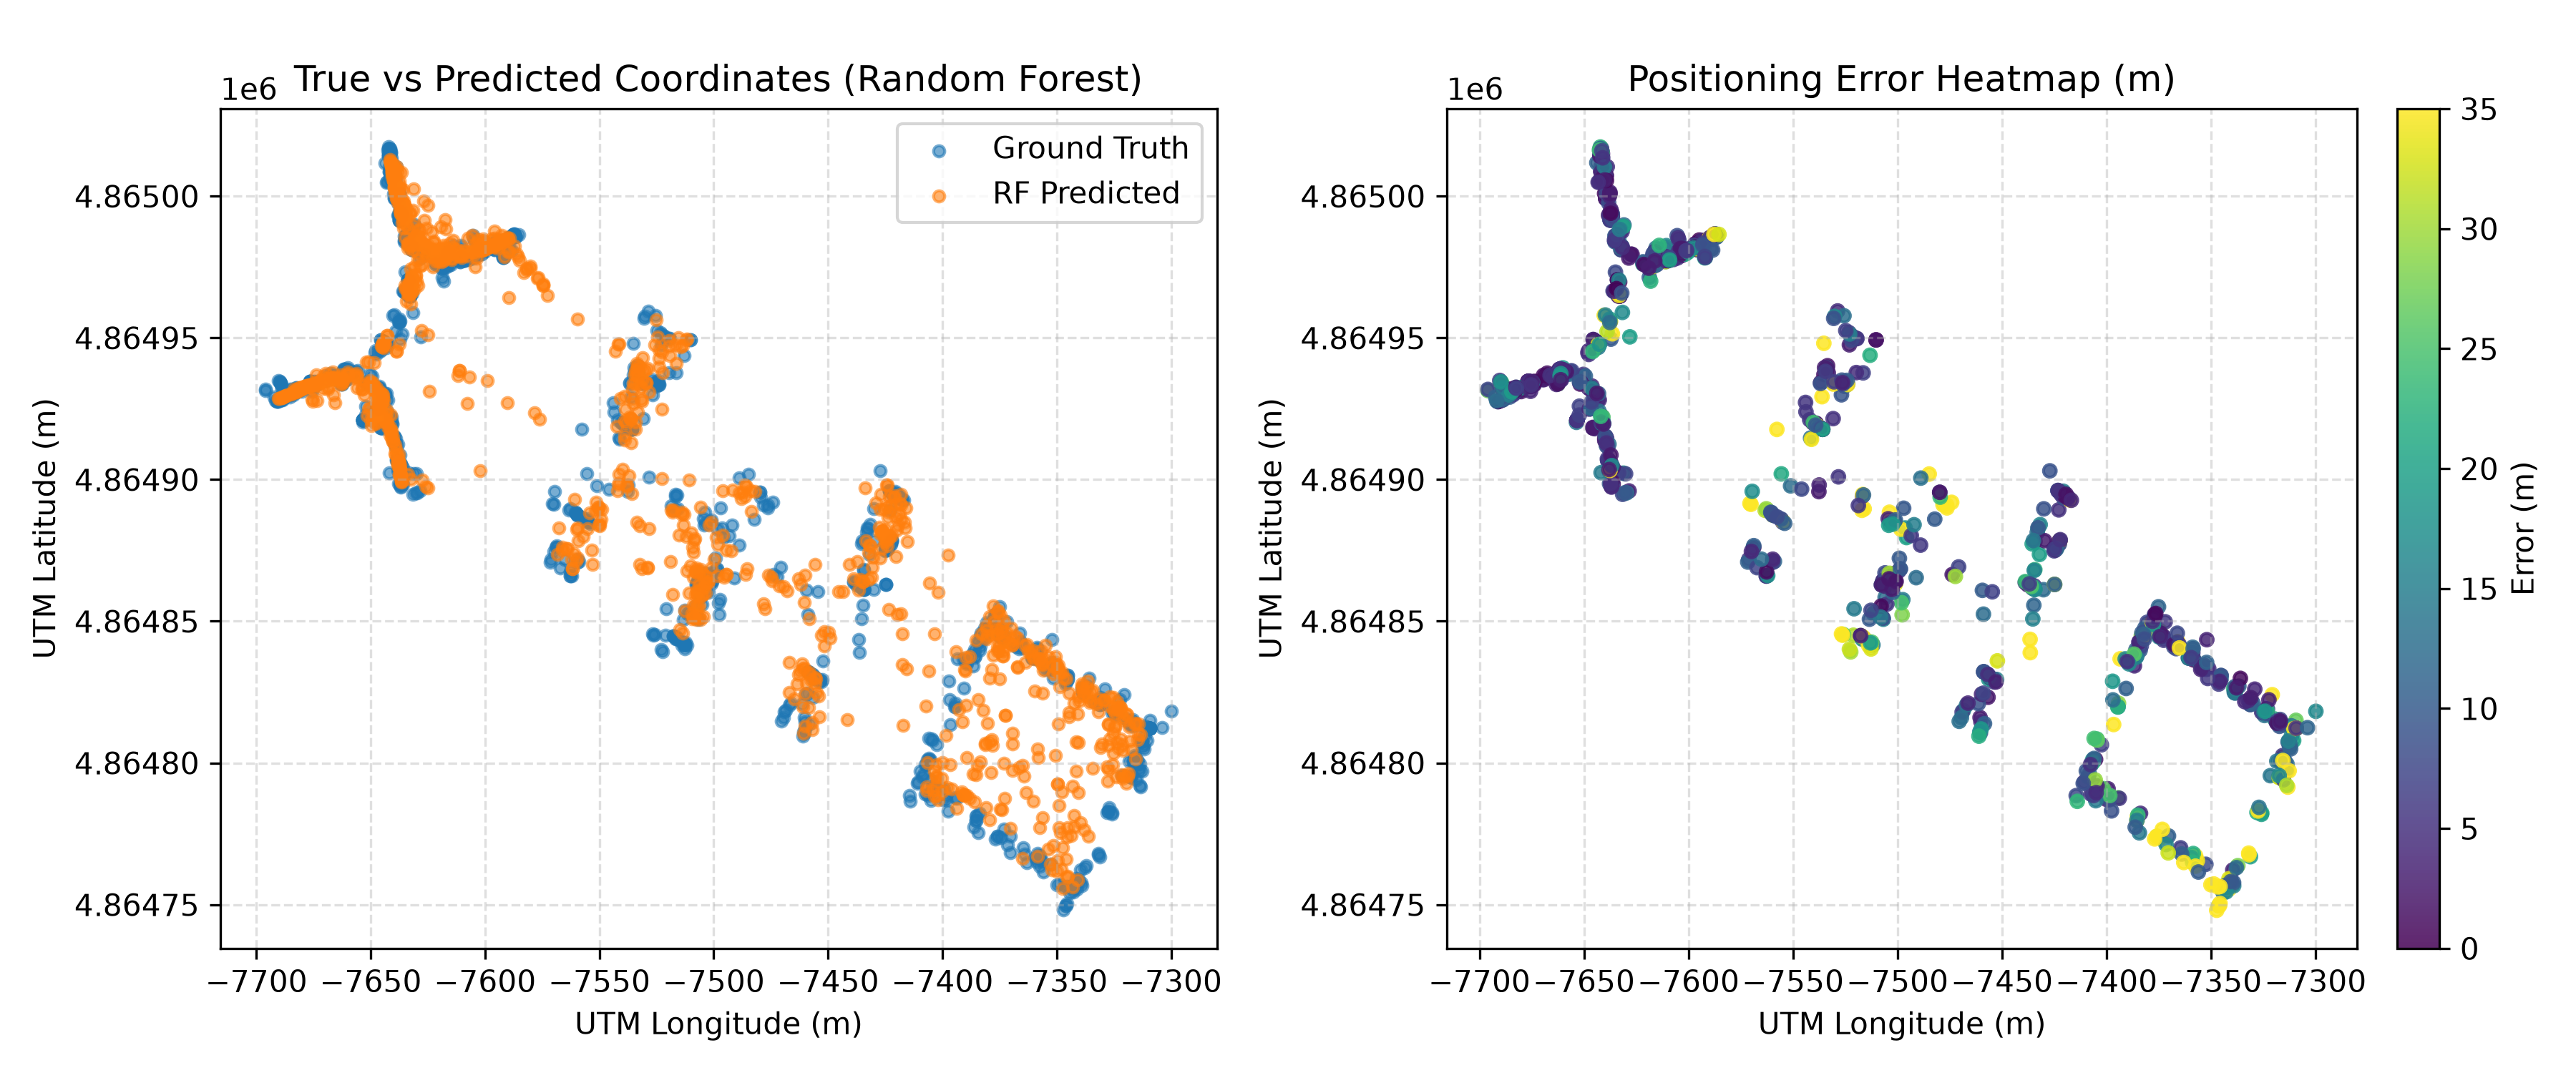
\includegraphics[width=0.9\textwidth]{figures/classical_spatial_errors.png}
  \caption{Spatial error visualization for Random Forest on the validation set: (left) True vs predicted UTM coordinates; (right) Positioning error heatmap across campus buildings.}
  \label{fig:spatial-errors}
\end{figure*}

% ─── 5.5 ─────────────────────────────────────────────────────────────────────
\subsection{Error Analysis and Distribution Shift}

\paragraph{Confusion Matrices.}
Fig.~\ref{fig:confusion-matrices} presents the confusion matrices for Random Forest. Building classification is near flawless ($99.91\%$), with only a single sample misclassified between adjacent buildings. Floor misclassifications occur almost exclusively between adjacent vertical floors ($\pm 1$ level), attributable to vertical RF signal leakage through concrete slabs.

\begin{figure}[t]
  \centering
  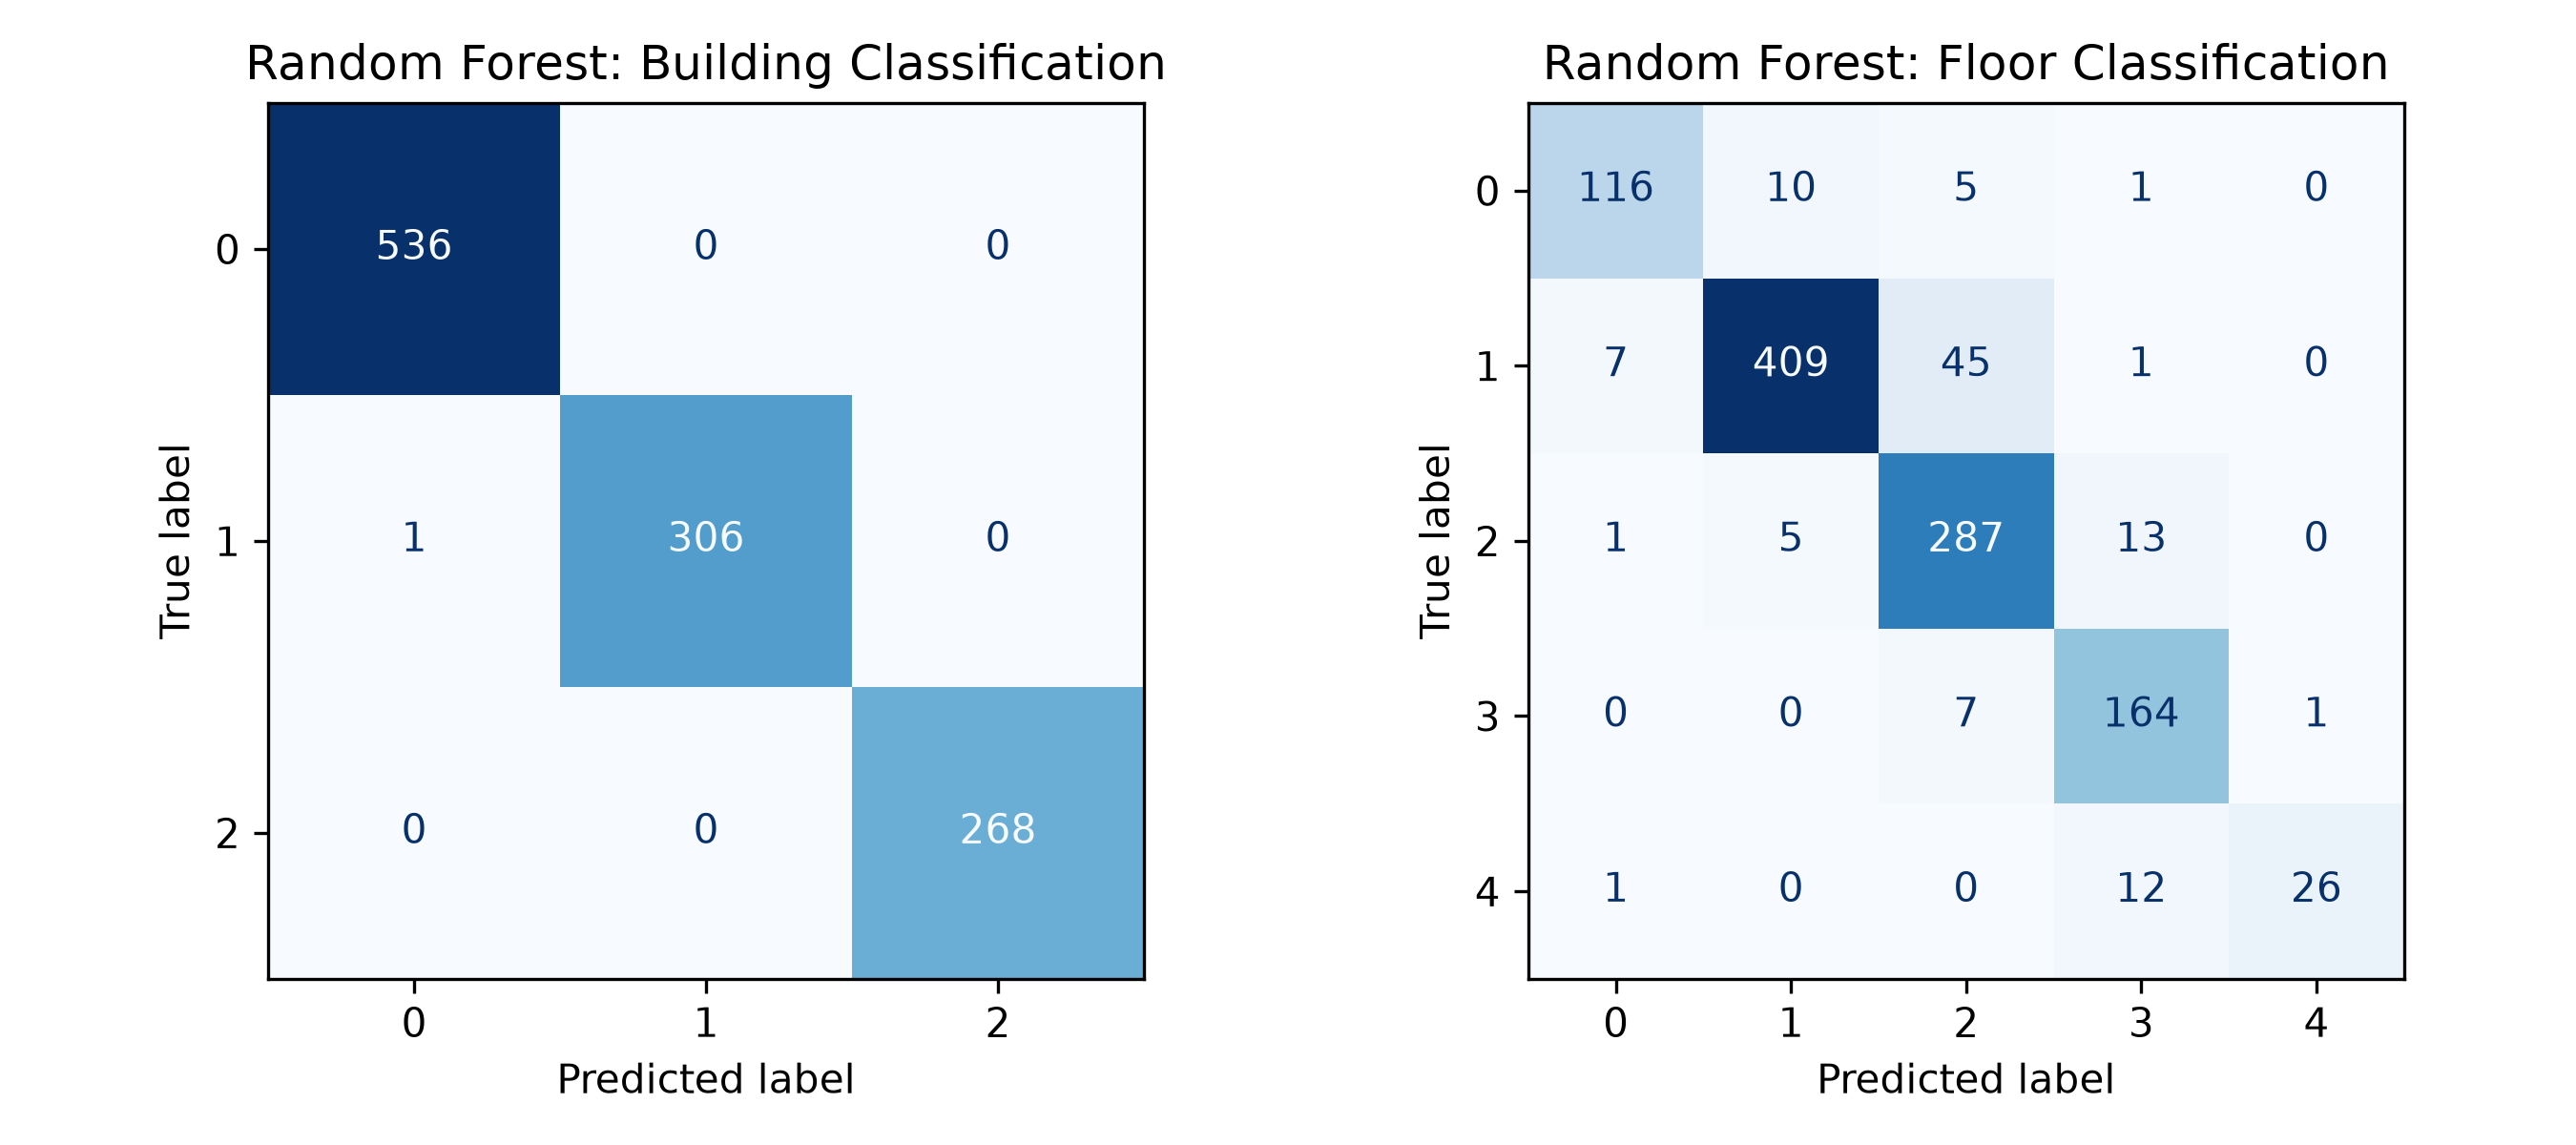
\includegraphics[width=\columnwidth]{figures/classical_confusion_matrices.png}
  \caption{Confusion matrices for Random Forest on building and floor classification.}
  \label{fig:confusion-matrices}
\end{figure}

\paragraph{Spatial Distribution of Positioning Error.}
Fig.~\ref{fig:spatial-errors} illustrates the spatial mapping of predictions. Errors are concentrated along building boundaries, open atriums, and corners where multipath interference is elevated and fewer APs provide line-of-sight coverage.

\paragraph{Quantifying Overfitting and Temporal Shift.}
A central viva topic is the gap between training cross-validation error ($\approx 4.5$~m) and validation error ($\approx 12.3$~m). This discrepancy is not attributable to model overfitting in the classical sense, but rather to \textbf{dataset distribution shift}:
\begin{enumerate}
  \item \textbf{Temporal Gap:} Validation fingerprints were gathered 4 months after training fingerprints, during which indoor access point operational states, transmission power, and building clutter shifted.
  \item \textbf{Hardware Heterogeneity:} The validation set introduces new smartphone models with distinct antenna sensitivity profiles.
\end{enumerate}

% ─── 5.6 ─────────────────────────────────────────────────────────────────────
\subsection{Feature Importance and Interpretability}

\begin{figure}[t]
  \centering
  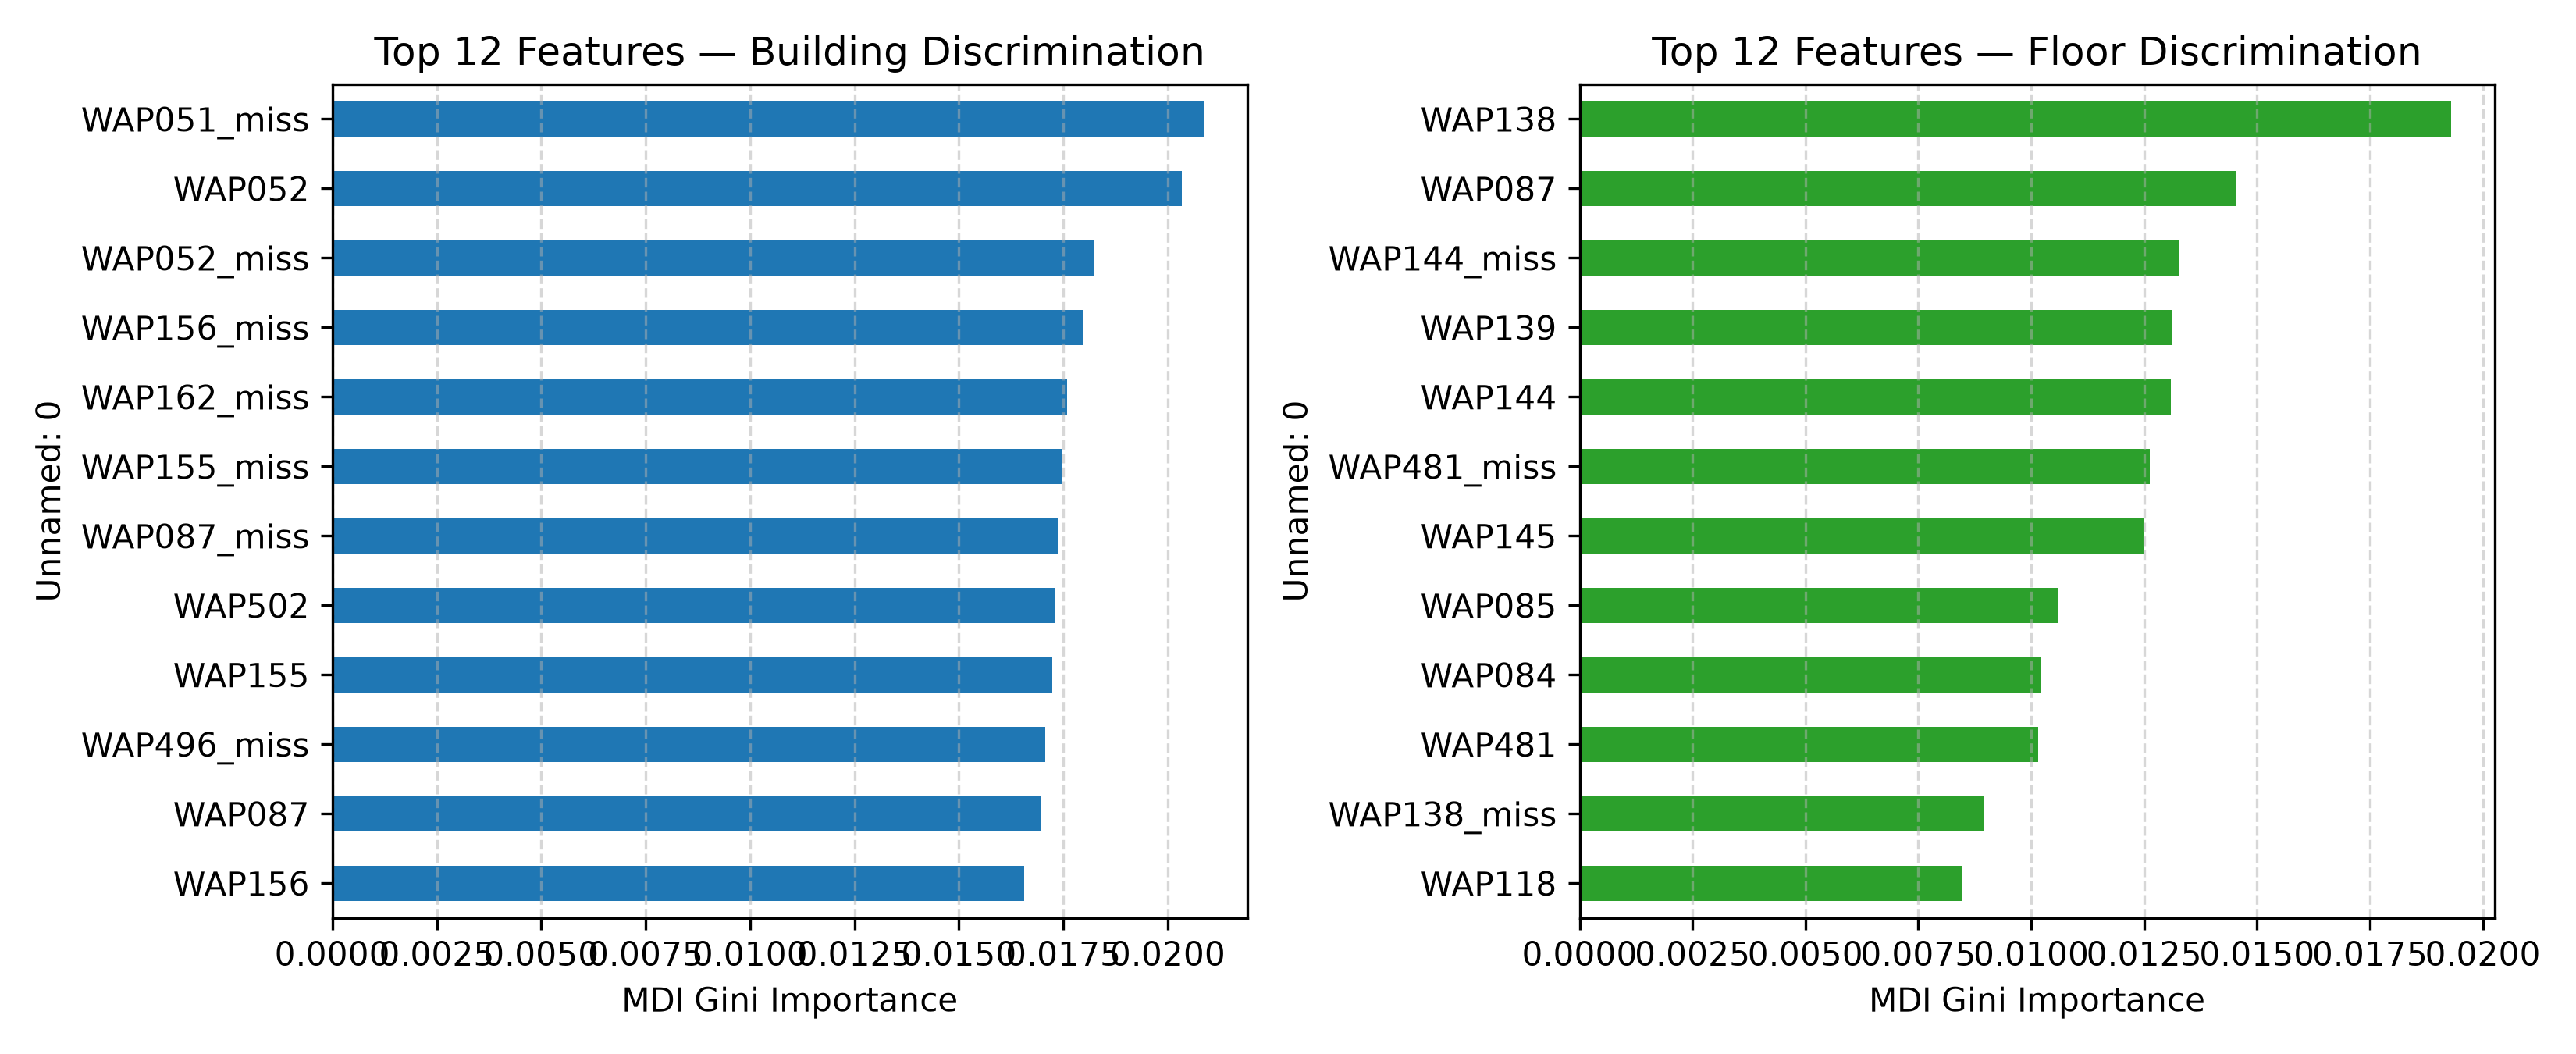
\includegraphics[width=\columnwidth]{figures/classical_feature_importance.png}
  \caption{Mean Decrease in Impurity (Gini Importance) for the top 12 features in building and floor Random Forest models.}
  \label{fig:feature-importance}
\end{figure}

Fig.~\ref{fig:feature-importance} plots the Mean Decrease in Impurity (MDI) for the top features. Building discrimination is dominated by localized access points such as \texttt{WAP248}, \texttt{WAP011}, and \texttt{WAP286}, which exhibit high transmission power confined to specific building footprints. Floor classification relies on access points mounted near vertical elevator shafts and central stairwells. Detection indicators account for over $35\%$ of total node split selections, confirming that the binary presence or absence of a transmitter is as informative as continuous signal strength.
